% Options for packages loaded elsewhere
\PassOptionsToPackage{unicode}{hyperref}
\PassOptionsToPackage{hyphens}{url}
\PassOptionsToPackage{dvipsnames,svgnames,x11names}{xcolor}
%
\documentclass[
  letterpaper,
  DIV=11,
  numbers=noendperiod]{scrreprt}

\usepackage{amsmath,amssymb}
\usepackage{iftex}
\ifPDFTeX
  \usepackage[T1]{fontenc}
  \usepackage[utf8]{inputenc}
  \usepackage{textcomp} % provide euro and other symbols
\else % if luatex or xetex
  \usepackage{unicode-math}
  \defaultfontfeatures{Scale=MatchLowercase}
  \defaultfontfeatures[\rmfamily]{Ligatures=TeX,Scale=1}
\fi
\usepackage{lmodern}
\ifPDFTeX\else  
    % xetex/luatex font selection
\fi
% Use upquote if available, for straight quotes in verbatim environments
\IfFileExists{upquote.sty}{\usepackage{upquote}}{}
\IfFileExists{microtype.sty}{% use microtype if available
  \usepackage[]{microtype}
  \UseMicrotypeSet[protrusion]{basicmath} % disable protrusion for tt fonts
}{}
\makeatletter
\@ifundefined{KOMAClassName}{% if non-KOMA class
  \IfFileExists{parskip.sty}{%
    \usepackage{parskip}
  }{% else
    \setlength{\parindent}{0pt}
    \setlength{\parskip}{6pt plus 2pt minus 1pt}}
}{% if KOMA class
  \KOMAoptions{parskip=half}}
\makeatother
\usepackage{xcolor}
\setlength{\emergencystretch}{3em} % prevent overfull lines
\setcounter{secnumdepth}{5}
% Make \paragraph and \subparagraph free-standing
\ifx\paragraph\undefined\else
  \let\oldparagraph\paragraph
  \renewcommand{\paragraph}[1]{\oldparagraph{#1}\mbox{}}
\fi
\ifx\subparagraph\undefined\else
  \let\oldsubparagraph\subparagraph
  \renewcommand{\subparagraph}[1]{\oldsubparagraph{#1}\mbox{}}
\fi

\usepackage{color}
\usepackage{fancyvrb}
\newcommand{\VerbBar}{|}
\newcommand{\VERB}{\Verb[commandchars=\\\{\}]}
\DefineVerbatimEnvironment{Highlighting}{Verbatim}{commandchars=\\\{\}}
% Add ',fontsize=\small' for more characters per line
\usepackage{framed}
\definecolor{shadecolor}{RGB}{241,243,245}
\newenvironment{Shaded}{\begin{snugshade}}{\end{snugshade}}
\newcommand{\AlertTok}[1]{\textcolor[rgb]{0.68,0.00,0.00}{#1}}
\newcommand{\AnnotationTok}[1]{\textcolor[rgb]{0.37,0.37,0.37}{#1}}
\newcommand{\AttributeTok}[1]{\textcolor[rgb]{0.40,0.45,0.13}{#1}}
\newcommand{\BaseNTok}[1]{\textcolor[rgb]{0.68,0.00,0.00}{#1}}
\newcommand{\BuiltInTok}[1]{\textcolor[rgb]{0.00,0.23,0.31}{#1}}
\newcommand{\CharTok}[1]{\textcolor[rgb]{0.13,0.47,0.30}{#1}}
\newcommand{\CommentTok}[1]{\textcolor[rgb]{0.37,0.37,0.37}{#1}}
\newcommand{\CommentVarTok}[1]{\textcolor[rgb]{0.37,0.37,0.37}{\textit{#1}}}
\newcommand{\ConstantTok}[1]{\textcolor[rgb]{0.56,0.35,0.01}{#1}}
\newcommand{\ControlFlowTok}[1]{\textcolor[rgb]{0.00,0.23,0.31}{#1}}
\newcommand{\DataTypeTok}[1]{\textcolor[rgb]{0.68,0.00,0.00}{#1}}
\newcommand{\DecValTok}[1]{\textcolor[rgb]{0.68,0.00,0.00}{#1}}
\newcommand{\DocumentationTok}[1]{\textcolor[rgb]{0.37,0.37,0.37}{\textit{#1}}}
\newcommand{\ErrorTok}[1]{\textcolor[rgb]{0.68,0.00,0.00}{#1}}
\newcommand{\ExtensionTok}[1]{\textcolor[rgb]{0.00,0.23,0.31}{#1}}
\newcommand{\FloatTok}[1]{\textcolor[rgb]{0.68,0.00,0.00}{#1}}
\newcommand{\FunctionTok}[1]{\textcolor[rgb]{0.28,0.35,0.67}{#1}}
\newcommand{\ImportTok}[1]{\textcolor[rgb]{0.00,0.46,0.62}{#1}}
\newcommand{\InformationTok}[1]{\textcolor[rgb]{0.37,0.37,0.37}{#1}}
\newcommand{\KeywordTok}[1]{\textcolor[rgb]{0.00,0.23,0.31}{#1}}
\newcommand{\NormalTok}[1]{\textcolor[rgb]{0.00,0.23,0.31}{#1}}
\newcommand{\OperatorTok}[1]{\textcolor[rgb]{0.37,0.37,0.37}{#1}}
\newcommand{\OtherTok}[1]{\textcolor[rgb]{0.00,0.23,0.31}{#1}}
\newcommand{\PreprocessorTok}[1]{\textcolor[rgb]{0.68,0.00,0.00}{#1}}
\newcommand{\RegionMarkerTok}[1]{\textcolor[rgb]{0.00,0.23,0.31}{#1}}
\newcommand{\SpecialCharTok}[1]{\textcolor[rgb]{0.37,0.37,0.37}{#1}}
\newcommand{\SpecialStringTok}[1]{\textcolor[rgb]{0.13,0.47,0.30}{#1}}
\newcommand{\StringTok}[1]{\textcolor[rgb]{0.13,0.47,0.30}{#1}}
\newcommand{\VariableTok}[1]{\textcolor[rgb]{0.07,0.07,0.07}{#1}}
\newcommand{\VerbatimStringTok}[1]{\textcolor[rgb]{0.13,0.47,0.30}{#1}}
\newcommand{\WarningTok}[1]{\textcolor[rgb]{0.37,0.37,0.37}{\textit{#1}}}

\providecommand{\tightlist}{%
  \setlength{\itemsep}{0pt}\setlength{\parskip}{0pt}}\usepackage{longtable,booktabs,array}
\usepackage{calc} % for calculating minipage widths
% Correct order of tables after \paragraph or \subparagraph
\usepackage{etoolbox}
\makeatletter
\patchcmd\longtable{\par}{\if@noskipsec\mbox{}\fi\par}{}{}
\makeatother
% Allow footnotes in longtable head/foot
\IfFileExists{footnotehyper.sty}{\usepackage{footnotehyper}}{\usepackage{footnote}}
\makesavenoteenv{longtable}
\usepackage{graphicx}
\makeatletter
\def\maxwidth{\ifdim\Gin@nat@width>\linewidth\linewidth\else\Gin@nat@width\fi}
\def\maxheight{\ifdim\Gin@nat@height>\textheight\textheight\else\Gin@nat@height\fi}
\makeatother
% Scale images if necessary, so that they will not overflow the page
% margins by default, and it is still possible to overwrite the defaults
% using explicit options in \includegraphics[width, height, ...]{}
\setkeys{Gin}{width=\maxwidth,height=\maxheight,keepaspectratio}
% Set default figure placement to htbp
\makeatletter
\def\fps@figure{htbp}
\makeatother

\KOMAoption{captions}{tableheading}
\makeatletter
\@ifpackageloaded{tcolorbox}{}{\usepackage[skins,breakable]{tcolorbox}}
\@ifpackageloaded{fontawesome5}{}{\usepackage{fontawesome5}}
\definecolor{quarto-callout-color}{HTML}{909090}
\definecolor{quarto-callout-note-color}{HTML}{0758E5}
\definecolor{quarto-callout-important-color}{HTML}{CC1914}
\definecolor{quarto-callout-warning-color}{HTML}{EB9113}
\definecolor{quarto-callout-tip-color}{HTML}{00A047}
\definecolor{quarto-callout-caution-color}{HTML}{FC5300}
\definecolor{quarto-callout-color-frame}{HTML}{acacac}
\definecolor{quarto-callout-note-color-frame}{HTML}{4582ec}
\definecolor{quarto-callout-important-color-frame}{HTML}{d9534f}
\definecolor{quarto-callout-warning-color-frame}{HTML}{f0ad4e}
\definecolor{quarto-callout-tip-color-frame}{HTML}{02b875}
\definecolor{quarto-callout-caution-color-frame}{HTML}{fd7e14}
\makeatother
\makeatletter
\@ifpackageloaded{bookmark}{}{\usepackage{bookmark}}
\makeatother
\makeatletter
\@ifpackageloaded{caption}{}{\usepackage{caption}}
\AtBeginDocument{%
\ifdefined\contentsname
  \renewcommand*\contentsname{Table of contents}
\else
  \newcommand\contentsname{Table of contents}
\fi
\ifdefined\listfigurename
  \renewcommand*\listfigurename{List of Figures}
\else
  \newcommand\listfigurename{List of Figures}
\fi
\ifdefined\listtablename
  \renewcommand*\listtablename{List of Tables}
\else
  \newcommand\listtablename{List of Tables}
\fi
\ifdefined\figurename
  \renewcommand*\figurename{Figure}
\else
  \newcommand\figurename{Figure}
\fi
\ifdefined\tablename
  \renewcommand*\tablename{Table}
\else
  \newcommand\tablename{Table}
\fi
}
\@ifpackageloaded{float}{}{\usepackage{float}}
\floatstyle{ruled}
\@ifundefined{c@chapter}{\newfloat{codelisting}{h}{lop}}{\newfloat{codelisting}{h}{lop}[chapter]}
\floatname{codelisting}{Listing}
\newcommand*\listoflistings{\listof{codelisting}{List of Listings}}
\makeatother
\makeatletter
\makeatother
\makeatletter
\@ifpackageloaded{caption}{}{\usepackage{caption}}
\@ifpackageloaded{subcaption}{}{\usepackage{subcaption}}
\makeatother
\ifLuaTeX
  \usepackage{selnolig}  % disable illegal ligatures
\fi
\usepackage{bookmark}

\IfFileExists{xurl.sty}{\usepackage{xurl}}{} % add URL line breaks if available
\urlstyle{same} % disable monospaced font for URLs
\hypersetup{
  pdftitle={Workspace},
  colorlinks=true,
  linkcolor={blue},
  filecolor={Maroon},
  citecolor={Blue},
  urlcolor={Blue},
  pdfcreator={LaTeX via pandoc}}

\title{Workspace}
\author{}
\date{}

\begin{document}
\maketitle

\renewcommand*\contentsname{Table of contents}
{
\hypersetup{linkcolor=}
\setcounter{tocdepth}{2}
\tableofcontents
}
\bookmarksetup{startatroot}

\chapter*{Welcome}\label{welcome}
\addcontentsline{toc}{chapter}{Welcome}

\markboth{Welcome}{Welcome}

This Quarto Book\footnote{\href{https://quarto.org/docs/books/}{Quarto
  Books Documentation}} is a workspace for the notes and projects of the
programming/scripting languages that I am learning.

\part{Notebooks}

This section contains notes for the programming/scripting languages that
I am learning.

\chapter{R}\label{r}

\section*{Clear Workspace, DON'T EDIT}\label{clear-workspace-dont-edit}
\addcontentsline{toc}{section}{Clear Workspace, DON'T EDIT}

\markright{Clear Workspace, DON'T EDIT}

Always start by clearing the workspace. This ensure objects created in
other files are not used used here.

\begin{Shaded}
\begin{Highlighting}[]
\FunctionTok{rm}\NormalTok{(}\AttributeTok{list =} \FunctionTok{ls}\NormalTok{())}
\end{Highlighting}
\end{Shaded}

\section*{List Used Packages, EDIT}\label{list-used-packages-edit}
\addcontentsline{toc}{section}{List Used Packages, EDIT}

\markright{List Used Packages, EDIT}

List all the packages that will be used in chunk below.

\begin{Shaded}
\begin{Highlighting}[]
\NormalTok{packages }\OtherTok{\textless{}{-}} \FunctionTok{c}\NormalTok{(}\StringTok{"here"}\NormalTok{, }\StringTok{"tidyverse"}\NormalTok{, }\StringTok{"janitor"}\NormalTok{)}
\end{Highlighting}
\end{Shaded}

\section*{Load Packages, DON'T EDIT}\label{sec-packages}
\addcontentsline{toc}{section}{Load Packages, DON'T EDIT}

\markright{Load Packages, DON'T EDIT}

\subsection*{Install Missing}\label{install-missing}
\addcontentsline{toc}{subsection}{Install Missing}

Any missing package will be installed automatically. This ensure
smoother execution when run by others.

\begin{Shaded}
\begin{Highlighting}[]
\CommentTok{\# Do NOT modify}
\FunctionTok{install.packages}\NormalTok{(}\FunctionTok{setdiff}\NormalTok{(packages, }\FunctionTok{rownames}\NormalTok{(}\FunctionTok{installed.packages}\NormalTok{())))}
\end{Highlighting}
\end{Shaded}

\subsection*{Load}\label{load}
\addcontentsline{toc}{subsection}{Load}

Load all packages

\begin{Shaded}
\begin{Highlighting}[]
\CommentTok{\# Do NOT modify}
\FunctionTok{lapply}\NormalTok{(packages, require, }\AttributeTok{character.only =} \ConstantTok{TRUE}\NormalTok{)}
\end{Highlighting}
\end{Shaded}

\begin{verbatim}
[[1]]
[1] TRUE
\end{verbatim}

\section{General Notes}\label{general-notes}

\begin{itemize}
\tightlist
\item
  When writing R code, create a project instead of a file which will
  enable saving the workspace settings
\item
  An R package usually includes:

  \begin{enumerate}
  \def\labelenumi{\alph{enumi}.}
  \tightlist
  \item
    reusable functions
  \item
    documentation describing how to use the function
  \item
    sample data
  \end{enumerate}
\item
  Before running a project, clear the objects in its workspace
  environment to avoid mixing up objects created in other files. This
  can be done either:

  \begin{enumerate}
  \def\labelenumi{\alph{enumi}.}
  \tightlist
  \item
    pragmatically as shown below OR
  \item
    Environment window -\textgreater{} Broom icon
  \end{enumerate}
\end{itemize}

\section{Data Types}\label{data-types}

\begin{itemize}
\tightlist
\item
  character
\item
  numeric
\item
  logical
\item
  raw
\item
  imaginary numbers
\end{itemize}

To know the datatype of an object, run the command:

\begin{Shaded}
\begin{Highlighting}[]
\FunctionTok{class}\NormalTok{(x) }\CommentTok{\# give the data type of x}
\end{Highlighting}
\end{Shaded}

To know the type of the variables of each variable.

\begin{Shaded}
\begin{Highlighting}[]
\NormalTok{x }\SpecialCharTok{|\textgreater{}} 
  \FunctionTok{slice}\NormalTok{(}\DecValTok{0}\NormalTok{) }\SpecialCharTok{|\textgreater{}} 
  \FunctionTok{glimpse}\NormalTok{()}
\end{Highlighting}
\end{Shaded}

\subsection{Mixing Data Types}\label{mixing-data-types}

\begin{itemize}
\tightlist
\item
  character + numeric --\textgreater{} character
\item
  numeric + logical --\textgreater{} numeric
\item
  numeric + character + logical --\textgreater{} character
\end{itemize}

\section{Data Structures}\label{data-structures}

\begin{itemize}
\tightlist
\item
  \textbf{vector}: hold single type of data
\end{itemize}

\begin{tcolorbox}[enhanced jigsaw, coltitle=black, opacityback=0, colback=white, title=\textcolor{quarto-callout-note-color}{\faInfo}\hspace{0.5em}{Creating Vector}, titlerule=0mm, bottomtitle=1mm, arc=.35mm, breakable, colbacktitle=quarto-callout-note-color!10!white, toptitle=1mm, left=2mm, bottomrule=.15mm, opacitybacktitle=0.6, toprule=.15mm, leftrule=.75mm, colframe=quarto-callout-note-color-frame, rightrule=.15mm]

The \texttt{c()} function (\textbf{c}ombine multiple elements) can be
used to create vectors in R.

\begin{verbatim}
x <- c(1, 2, 3, 4)
\end{verbatim}

\end{tcolorbox}

\begin{itemize}
\tightlist
\item
  \textbf{matrix}: 2D vector
\item
  \textbf{array}: nD vector
\item
  \textbf{list}: generic vector, can hold mixed type of data, eg, one
  element can a character, another a list of integers, and the third
  could be a logical
\item
  \textbf{data frame}: table where columns represent vectors
\item
  \textbf{tibbles}: data frames, but slightly tweaked to work better
  with \texttt{tidyverse}--when printing tibbles, only the first few
  columns that fit into the screen will be shown
\end{itemize}

\begin{tcolorbox}[enhanced jigsaw, coltitle=black, opacityback=0, colback=white, title=\textcolor{quarto-callout-note-color}{\faInfo}\hspace{0.5em}{Printing tibble All Columns}, titlerule=0mm, bottomtitle=1mm, arc=.35mm, breakable, colbacktitle=quarto-callout-note-color!10!white, toptitle=1mm, left=2mm, bottomrule=.15mm, opacitybacktitle=0.6, toprule=.15mm, leftrule=.75mm, colframe=quarto-callout-note-color-frame, rightrule=.15mm]

To force the \texttt{print()} function to print all the columns of a
\texttt{tibble}, set the \texttt{width} parameter to \texttt{Inf} as
follows:

\begin{Shaded}
\begin{Highlighting}[]
\FunctionTok{print}\NormalTok{(ds, }\AttributeTok{width =} \ConstantTok{Inf}\NormalTok{)}
\end{Highlighting}
\end{Shaded}

\end{tcolorbox}

To construct small tibble by hand, use the \texttt{tribble} function as
follows:

\begin{Shaded}
\begin{Highlighting}[]
\NormalTok{df }\OtherTok{\textless{}{-}} \FunctionTok{tribble}\NormalTok{(}
  \SpecialCharTok{\textasciitilde{}}\NormalTok{var1, }\SpecialCharTok{\textasciitilde{}}\NormalTok{var2, }\SpecialCharTok{\textasciitilde{}}\NormalTok{var3}
  \StringTok{"A"}\NormalTok{, }\DecValTok{1}\NormalTok{, }\ConstantTok{TRUE}\NormalTok{,}
  \StringTok{"B"}\NormalTok{, }\DecValTok{2}\NormalTok{, }\ConstantTok{FALSE}\NormalTok{,}
  \StringTok{"C"}\NormalTok{, }\DecValTok{3}\NormalTok{, }\ConstantTok{TRUE}
\NormalTok{)}
\end{Highlighting}
\end{Shaded}

\begin{itemize}
\tightlist
\item
  \textbf{factor}
\end{itemize}

\begin{figure}

\centering{

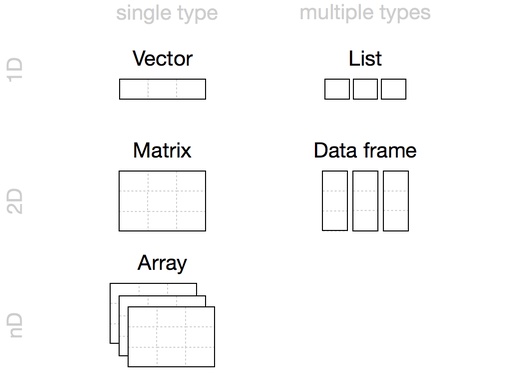
\includegraphics[width=1.71in,height=\textheight]{src/notebooks/../../images/datastructure.png}

}

\caption{\label{fig-datastructure}Common data structures in R ( taken
from \href{https://jjallaire.github.io/hopr/objects.html}{Grolemund,
2014})}

\end{figure}%

To know the data structure and length of the object, run the command:

\begin{Shaded}
\begin{Highlighting}[]
\FunctionTok{str}\NormalTok{(x) }\CommentTok{\# give the structure type of x}
\FunctionTok{length}\NormalTok{(x) }\CommentTok{\# length of structure}
\end{Highlighting}
\end{Shaded}

\section{Basics Operations}\label{basics-operations}

Assignment

\begin{Shaded}
\begin{Highlighting}[]
\NormalTok{x }\OtherTok{\textless{}{-}} \DecValTok{3} \CommentTok{\# assign 3 to x (x gets 3)}
\NormalTok{(x }\OtherTok{\textless{}{-}} \DecValTok{3}\NormalTok{) }\CommentTok{\# assign 3 to x (x gets 3) \& print the result to console}
\end{Highlighting}
\end{Shaded}

\begin{verbatim}
[1] 3
\end{verbatim}

Getting Help

\begin{Shaded}
\begin{Highlighting}[]
\FunctionTok{args}\NormalTok{(round) }\CommentTok{\# print the argument list of function}
\NormalTok{?round }\CommentTok{\# show documentation of function in Help window}
\end{Highlighting}
\end{Shaded}

Dealing with Structure

\begin{Shaded}
\begin{Highlighting}[]
\CommentTok{\# concatenate set of values to create vector}
\NormalTok{weight\_g }\OtherTok{\textless{}{-}} \FunctionTok{c}\NormalTok{(}\DecValTok{50}\NormalTok{, }\DecValTok{60}\NormalTok{, }\DecValTok{3}\NormalTok{, }\DecValTok{9}\NormalTok{)}
\NormalTok{animals }\OtherTok{\textless{}{-}} \FunctionTok{c}\NormalTok{(}\StringTok{"dog"}\NormalTok{, }\StringTok{"bat"}\NormalTok{, }\StringTok{"cat"}\NormalTok{)}

\CommentTok{\# utilizing logical values to pull specific values}
\NormalTok{weight\_g[weight\_g }\SpecialCharTok{\textless{}} \DecValTok{10} \SpecialCharTok{\&}\NormalTok{ weight\_g }\SpecialCharTok{\textgreater{}} \DecValTok{60} \SpecialCharTok{|}\NormalTok{ weight\_g }\SpecialCharTok{==} \DecValTok{50}\NormalTok{]}
\end{Highlighting}
\end{Shaded}

\begin{verbatim}
[1] 50
\end{verbatim}

\begin{Shaded}
\begin{Highlighting}[]
\CommentTok{\# pull dog \& cat records}
\NormalTok{animals[animals }\SpecialCharTok{\%in\%} \FunctionTok{c}\NormalTok{(}\StringTok{"dog"}\NormalTok{, }\StringTok{"cat"}\NormalTok{)]}
\end{Highlighting}
\end{Shaded}

\begin{verbatim}
[1] "dog" "cat"
\end{verbatim}

\begin{Shaded}
\begin{Highlighting}[]
\NormalTok{animals[animals }\SpecialCharTok{==} \StringTok{"dog"} \SpecialCharTok{|}\NormalTok{ animals }\SpecialCharTok{==} \StringTok{"cat"}\NormalTok{]}
\end{Highlighting}
\end{Shaded}

\begin{verbatim}
[1] "dog" "cat"
\end{verbatim}

Statistics

\begin{Shaded}
\begin{Highlighting}[]
\CommentTok{\# signaling missing data using NA}
\NormalTok{heights }\OtherTok{\textless{}{-}} \FunctionTok{c}\NormalTok{(}\DecValTok{2}\NormalTok{, }\DecValTok{3}\NormalTok{, }\ConstantTok{NA}\NormalTok{, }\DecValTok{4}\NormalTok{)}

\CommentTok{\# get mean while ignoring missing data}
\FunctionTok{mean}\NormalTok{(heights, }\AttributeTok{na.rm =} \ConstantTok{TRUE}\NormalTok{)}
\end{Highlighting}
\end{Shaded}

\begin{verbatim}
[1] 3
\end{verbatim}

\begin{Shaded}
\begin{Highlighting}[]
\CommentTok{\# how to use mean}
\CommentTok{\# ?mean}
\end{Highlighting}
\end{Shaded}

\section{Exploratory Operations}\label{exploratory-operations}

The \texttt{here} package makes it easy to point to files starting from
the project main directory.

\begin{Shaded}
\begin{Highlighting}[]
\FunctionTok{library}\NormalTok{(}\StringTok{"here"}\NormalTok{, }\StringTok{"janitor"}\NormalTok{)}
\end{Highlighting}
\end{Shaded}

Loading file from repository and saving it locally on disk. It is always
a good idea to structure the workspace--for more information, see
\href{http://journals.plos.org/plosbiology/article?id=10.1371/journal.pbio.1001745}{Best
Practices for Scientific Computing paper}.

\begin{Shaded}
\begin{Highlighting}[]
\FunctionTok{download.file}\NormalTok{(}
  \AttributeTok{url =} \StringTok{"https://ndownloader.figshare.com/files/2292169"}\NormalTok{,}
  \AttributeTok{destfile =} \FunctionTok{here}\NormalTok{(}\StringTok{"data"}\NormalTok{, }\StringTok{"portal\_data\_joined.csv"}\NormalTok{)}
\NormalTok{)}
\end{Highlighting}
\end{Shaded}

Load file to R as data frame

\begin{Shaded}
\begin{Highlighting}[]
\NormalTok{surveys }\OtherTok{\textless{}{-}} \FunctionTok{read.csv}\NormalTok{(}\FunctionTok{here}\NormalTok{(}\StringTok{"data"}\NormalTok{, }\StringTok{"portal\_data\_joined.csv"}\NormalTok{))}

\FunctionTok{glimpse}\NormalTok{(surveys)}
\end{Highlighting}
\end{Shaded}

\begin{verbatim}
Rows: 34,786
Columns: 13
$ record_id       <int> 1, 72, 224, 266, 349, 363, 435, 506, 588, 661, 748, 84~
$ month           <int> 7, 8, 9, 10, 11, 11, 12, 1, 2, 3, 4, 5, 6, 8, 9, 10, 1~
$ day             <int> 16, 19, 13, 16, 12, 12, 10, 8, 18, 11, 8, 6, 9, 5, 4, ~
$ year            <int> 1977, 1977, 1977, 1977, 1977, 1977, 1977, 1978, 1978, ~
$ plot_id         <int> 2, 2, 2, 2, 2, 2, 2, 2, 2, 2, 2, 2, 2, 2, 2, 2, 2, 2, ~
$ species_id      <chr> "NL", "NL", "NL", "NL", "NL", "NL", "NL", "NL", "NL", ~
$ sex             <chr> "M", "M", "", "", "", "", "", "", "M", "", "", "M", "M~
$ hindfoot_length <int> 32, 31, NA, NA, NA, NA, NA, NA, NA, NA, NA, 32, NA, 34~
$ weight          <int> NA, NA, NA, NA, NA, NA, NA, NA, 218, NA, NA, 204, 200,~
$ genus           <chr> "Neotoma", "Neotoma", "Neotoma", "Neotoma", "Neotoma",~
$ species         <chr> "albigula", "albigula", "albigula", "albigula", "albig~
$ taxa            <chr> "Rodent", "Rodent", "Rodent", "Rodent", "Rodent", "Rod~
$ plot_type       <chr> "Control", "Control", "Control", "Control", "Control",~
\end{verbatim}

Clean names

\begin{Shaded}
\begin{Highlighting}[]
\NormalTok{surveys }\OtherTok{\textless{}{-}}\NormalTok{ surveys }\SpecialCharTok{|\textgreater{}} 
\NormalTok{  janitor}\SpecialCharTok{::}\FunctionTok{clean\_names}\NormalTok{()}
\end{Highlighting}
\end{Shaded}

Inspecting data frame

\begin{Shaded}
\begin{Highlighting}[]
\FunctionTok{class}\NormalTok{(surveys) }\CommentTok{\# data type}
\end{Highlighting}
\end{Shaded}

\begin{verbatim}
[1] "data.frame"
\end{verbatim}

\begin{Shaded}
\begin{Highlighting}[]
\FunctionTok{str}\NormalTok{(surveys) }\CommentTok{\# structure}
\end{Highlighting}
\end{Shaded}

\begin{verbatim}
'data.frame':   34786 obs. of  13 variables:
 $ record_id      : int  1 72 224 266 349 363 435 506 588 661 ...
 $ month          : int  7 8 9 10 11 11 12 1 2 3 ...
 $ day            : int  16 19 13 16 12 12 10 8 18 11 ...
 $ year           : int  1977 1977 1977 1977 1977 1977 1977 1978 1978 1978 ...
 $ plot_id        : int  2 2 2 2 2 2 2 2 2 2 ...
 $ species_id     : chr  "NL" "NL" "NL" "NL" ...
 $ sex            : chr  "M" "M" "" "" ...
 $ hindfoot_length: int  32 31 NA NA NA NA NA NA NA NA ...
 $ weight         : int  NA NA NA NA NA NA NA NA 218 NA ...
 $ genus          : chr  "Neotoma" "Neotoma" "Neotoma" "Neotoma" ...
 $ species        : chr  "albigula" "albigula" "albigula" "albigula" ...
 $ taxa           : chr  "Rodent" "Rodent" "Rodent" "Rodent" ...
 $ plot_type      : chr  "Control" "Control" "Control" "Control" ...
\end{verbatim}

\begin{Shaded}
\begin{Highlighting}[]
\NormalTok{surveys }\SpecialCharTok{|\textgreater{}} 
  \FunctionTok{slice}\NormalTok{(}\DecValTok{0}\NormalTok{) }\SpecialCharTok{|\textgreater{}} 
  \FunctionTok{glimpse}\NormalTok{()}
\end{Highlighting}
\end{Shaded}

\begin{verbatim}
Rows: 0
Columns: 13
$ record_id       <int> 
$ month           <int> 
$ day             <int> 
$ year            <int> 
$ plot_id         <int> 
$ species_id      <chr> 
$ sex             <chr> 
$ hindfoot_length <int> 
$ weight          <int> 
$ genus           <chr> 
$ species         <chr> 
$ taxa            <chr> 
$ plot_type       <chr> 
\end{verbatim}

\begin{Shaded}
\begin{Highlighting}[]
\FunctionTok{dim}\NormalTok{(surveys) }\CommentTok{\# dimensions}
\end{Highlighting}
\end{Shaded}

\begin{verbatim}
[1] 34786    13
\end{verbatim}

\begin{Shaded}
\begin{Highlighting}[]
\FunctionTok{nrow}\NormalTok{(surveys)}
\end{Highlighting}
\end{Shaded}

\begin{verbatim}
[1] 34786
\end{verbatim}

\begin{Shaded}
\begin{Highlighting}[]
\FunctionTok{ncol}\NormalTok{(surveys)}
\end{Highlighting}
\end{Shaded}

\begin{verbatim}
[1] 13
\end{verbatim}

\begin{Shaded}
\begin{Highlighting}[]
\FunctionTok{summary}\NormalTok{(surveys)}
\end{Highlighting}
\end{Shaded}

\begin{verbatim}
   record_id         month             day            year         plot_id     
 Min.   :    1   Min.   : 1.000   Min.   : 1.0   Min.   :1977   Min.   : 1.00  
 1st Qu.: 8964   1st Qu.: 4.000   1st Qu.: 9.0   1st Qu.:1984   1st Qu.: 5.00  
 Median :17762   Median : 6.000   Median :16.0   Median :1990   Median :11.00  
 Mean   :17804   Mean   : 6.474   Mean   :16.1   Mean   :1990   Mean   :11.34  
 3rd Qu.:26655   3rd Qu.:10.000   3rd Qu.:23.0   3rd Qu.:1997   3rd Qu.:17.00  
 Max.   :35548   Max.   :12.000   Max.   :31.0   Max.   :2002   Max.   :24.00  
                                                                               
  species_id            sex            hindfoot_length     weight      
 Length:34786       Length:34786       Min.   : 2.00   Min.   :  4.00  
 Class :character   Class :character   1st Qu.:21.00   1st Qu.: 20.00  
 Mode  :character   Mode  :character   Median :32.00   Median : 37.00  
                                       Mean   :29.29   Mean   : 42.67  
                                       3rd Qu.:36.00   3rd Qu.: 48.00  
                                       Max.   :70.00   Max.   :280.00  
                                       NA's   :3348    NA's   :2503    
    genus             species              taxa            plot_type        
 Length:34786       Length:34786       Length:34786       Length:34786      
 Class :character   Class :character   Class :character   Class :character  
 Mode  :character   Mode  :character   Mode  :character   Mode  :character  
                                                                            
                                                                            
                                                                            
                                                                            
\end{verbatim}

Show first/last few objects/records/rows

\begin{Shaded}
\begin{Highlighting}[]
\FunctionTok{head}\NormalTok{(surveys)}
\end{Highlighting}
\end{Shaded}

\begin{verbatim}
  record_id month day year plot_id species_id sex hindfoot_length weight
1         1     7  16 1977       2         NL   M              32     NA
2        72     8  19 1977       2         NL   M              31     NA
3       224     9  13 1977       2         NL                  NA     NA
4       266    10  16 1977       2         NL                  NA     NA
5       349    11  12 1977       2         NL                  NA     NA
6       363    11  12 1977       2         NL                  NA     NA
    genus  species   taxa plot_type
1 Neotoma albigula Rodent   Control
2 Neotoma albigula Rodent   Control
3 Neotoma albigula Rodent   Control
4 Neotoma albigula Rodent   Control
5 Neotoma albigula Rodent   Control
6 Neotoma albigula Rodent   Control
\end{verbatim}

\begin{Shaded}
\begin{Highlighting}[]
\FunctionTok{tail}\NormalTok{(surveys)}
\end{Highlighting}
\end{Shaded}

\begin{verbatim}
      record_id month day year plot_id species_id sex hindfoot_length weight
34781     26787     9  27 1997       7         PL   F              21     16
34782     26966    10  25 1997       7         PL   M              20     16
34783     27185    11  22 1997       7         PL   F              21     22
34784     27792     5   2 1998       7         PL   F              20      8
34785     28806    11  21 1998       7         PX                  NA     NA
34786     30986     7   1 2000       7         PX                  NA     NA
            genus  species   taxa        plot_type
34781  Peromyscus leucopus Rodent Rodent Exclosure
34782  Peromyscus leucopus Rodent Rodent Exclosure
34783  Peromyscus leucopus Rodent Rodent Exclosure
34784  Peromyscus leucopus Rodent Rodent Exclosure
34785 Chaetodipus      sp. Rodent Rodent Exclosure
34786 Chaetodipus      sp. Rodent Rodent Exclosure
\end{verbatim}

\subsection{Retrieve specific
element/row/column}\label{retrieve-specific-elementrowcolumn}

\begin{Shaded}
\begin{Highlighting}[]
\NormalTok{surveys[}\DecValTok{1}\NormalTok{, }\DecValTok{1}\NormalTok{] }\CommentTok{\# element[1,1]}
\end{Highlighting}
\end{Shaded}

\begin{verbatim}
[1] 1
\end{verbatim}

\begin{Shaded}
\begin{Highlighting}[]
\NormalTok{surveys[}\DecValTok{1}\NormalTok{, ] }\CommentTok{\# row 1}
\end{Highlighting}
\end{Shaded}

\begin{verbatim}
  record_id month day year plot_id species_id sex hindfoot_length weight
1         1     7  16 1977       2         NL   M              32     NA
    genus  species   taxa plot_type
1 Neotoma albigula Rodent   Control
\end{verbatim}

\begin{Shaded}
\begin{Highlighting}[]
\FunctionTok{head}\NormalTok{(surveys[, }\DecValTok{1}\NormalTok{]) }\CommentTok{\# column 1}
\end{Highlighting}
\end{Shaded}

\begin{verbatim}
[1]   1  72 224 266 349 363
\end{verbatim}

\begin{Shaded}
\begin{Highlighting}[]
\FunctionTok{head}\NormalTok{(surveys}\SpecialCharTok{$}\NormalTok{sex) }\CommentTok{\# column by name}
\end{Highlighting}
\end{Shaded}

\begin{verbatim}
[1] "M" "M" ""  ""  ""  "" 
\end{verbatim}

\subsection{Dealing with factor (categorical)
columns}\label{dealing-with-factor-categorical-columns}

R convert columns that contain characters to factors by default. Factors
are treated as integer vectors. By default, R sorts levels in
alphabetical order.

\begin{Shaded}
\begin{Highlighting}[]
\FunctionTok{levels}\NormalTok{(surveys}\SpecialCharTok{$}\NormalTok{sex)}
\end{Highlighting}
\end{Shaded}

\begin{verbatim}
NULL
\end{verbatim}

\begin{Shaded}
\begin{Highlighting}[]
\FunctionTok{nlevels}\NormalTok{(surveys}\SpecialCharTok{$}\NormalTok{sex)}
\end{Highlighting}
\end{Shaded}

\begin{verbatim}
[1] 0
\end{verbatim}

Reorder factors (to get better plots)

\begin{Shaded}
\begin{Highlighting}[]
\NormalTok{surveys}\SpecialCharTok{$}\NormalTok{sex\_ordered }\OtherTok{\textless{}{-}} \FunctionTok{factor}\NormalTok{(surveys}\SpecialCharTok{$}\NormalTok{sex, }\AttributeTok{level =} \FunctionTok{c}\NormalTok{(}\StringTok{"F"}\NormalTok{, }\StringTok{"M"}\NormalTok{, }\StringTok{""}\NormalTok{))}
\FunctionTok{str}\NormalTok{(surveys}\SpecialCharTok{$}\NormalTok{sex\_ordered)}
\end{Highlighting}
\end{Shaded}

\begin{verbatim}
 Factor w/ 3 levels "F","M","": 2 2 3 3 3 3 3 3 2 3 ...
\end{verbatim}

\begin{Shaded}
\begin{Highlighting}[]
\FunctionTok{levels}\NormalTok{(surveys}\SpecialCharTok{$}\NormalTok{sex\_ordered)}
\end{Highlighting}
\end{Shaded}

\begin{verbatim}
[1] "F" "M" "" 
\end{verbatim}

\begin{Shaded}
\begin{Highlighting}[]
\FunctionTok{nlevels}\NormalTok{(surveys}\SpecialCharTok{$}\NormalTok{sex\_ordered)}
\end{Highlighting}
\end{Shaded}

\begin{verbatim}
[1] 3
\end{verbatim}

\subsection{Basic Plotting}\label{basic-plotting}

Histogram

\begin{Shaded}
\begin{Highlighting}[]
\CommentTok{\# plot(surveys$sex)  \# not possible}
\FunctionTok{plot}\NormalTok{(surveys}\SpecialCharTok{$}\NormalTok{sex\_ordered)}
\end{Highlighting}
\end{Shaded}

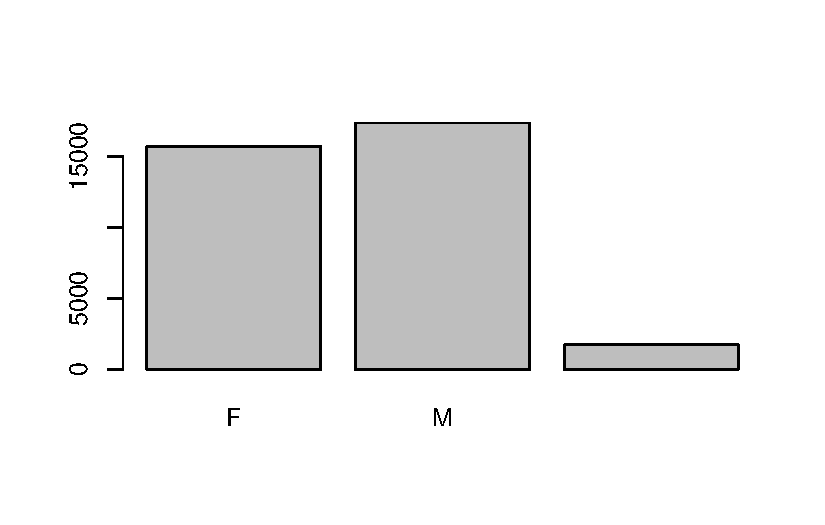
\includegraphics{src/notebooks/r_files/figure-pdf/unnamed-chunk-26-1.pdf}

Enhance the plot

\begin{Shaded}
\begin{Highlighting}[]
\FunctionTok{levels}\NormalTok{(surveys}\SpecialCharTok{$}\NormalTok{sex\_ordered)[}\DecValTok{1}\NormalTok{] }\OtherTok{\textless{}{-}} \StringTok{"Female"}
\FunctionTok{levels}\NormalTok{(surveys}\SpecialCharTok{$}\NormalTok{sex\_ordered)[}\DecValTok{2}\NormalTok{] }\OtherTok{\textless{}{-}} \StringTok{"Male"}
\FunctionTok{plot}\NormalTok{(surveys}\SpecialCharTok{$}\NormalTok{sex\_ordered)}
\end{Highlighting}
\end{Shaded}

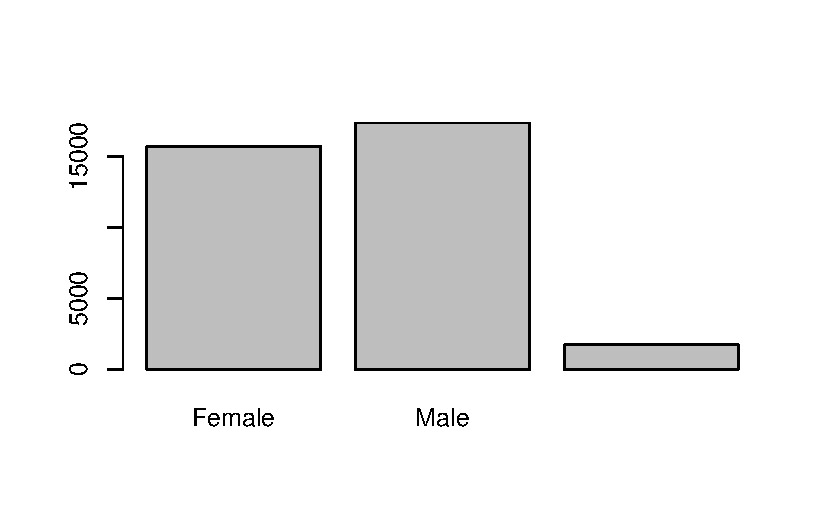
\includegraphics{src/notebooks/r_files/figure-pdf/unnamed-chunk-27-1.pdf}

\section{Data Manipulation}\label{data-manipulation}

\begin{itemize}
\tightlist
\item
  \texttt{tdlyr}

  \begin{itemize}
  \tightlist
  \item
    makes manipulation of data easier
  \item
    built to work with data frames directly
  \item
    can directly work with data stored in an external database which
    give the advantage of only bringing what we need to the memory to
    work on without having to bring the whole database
  \end{itemize}
\item
  \texttt{tidyr}

  \begin{itemize}
  \tightlist
  \item
    allows to swiftly convert b/w different data formats for plotting \&
    analysis in order to accommodate the different requirements by
    different functions

    \begin{itemize}
    \tightlist
    \item
      sometime we want one row per measurement
    \item
      other times we want the data aggregated like when plotting
    \end{itemize}
  \end{itemize}
\end{itemize}

Before using \texttt{tdlyr} and \texttt{tidyr}:

\begin{itemize}
\tightlist
\item
  Install \texttt{tidyverse} package: umbrella-package that install
  several packages (tidyr, dplyr, ggplot2 tibble, magrittr, etc.)
\item
  Load the package each session
\end{itemize}

Load packages

\begin{Shaded}
\begin{Highlighting}[]
\FunctionTok{library}\NormalTok{(}\StringTok{"tidyverse"}\NormalTok{)}
\end{Highlighting}
\end{Shaded}

Load \& inspect data

\begin{Shaded}
\begin{Highlighting}[]
\CommentTok{\# notice the \textquotesingle{}\_\textquotesingle{} instead of \textquotesingle{}.\textquotesingle{} of basic R}
\NormalTok{surveys }\OtherTok{\textless{}{-}} \FunctionTok{read\_csv}\NormalTok{(}\FunctionTok{here}\NormalTok{(}\StringTok{"data"}\NormalTok{, }\StringTok{"portal\_data\_joined.csv"}\NormalTok{))}
\end{Highlighting}
\end{Shaded}

\begin{verbatim}
Rows: 34786 Columns: 13
-- Column specification --------------------------------------------------------
Delimiter: ","
chr (6): species_id, sex, genus, species, taxa, plot_type
dbl (7): record_id, month, day, year, plot_id, hindfoot_length, weight

i Use `spec()` to retrieve the full column specification for this data.
i Specify the column types or set `show_col_types = FALSE` to quiet this message.
\end{verbatim}

\begin{Shaded}
\begin{Highlighting}[]
\FunctionTok{str}\NormalTok{(surveys) }\CommentTok{\# structure: tbl\_df (tibble)}
\end{Highlighting}
\end{Shaded}

\begin{verbatim}
spc_tbl_ [34,786 x 13] (S3: spec_tbl_df/tbl_df/tbl/data.frame)
 $ record_id      : num [1:34786] 1 72 224 266 349 363 435 506 588 661 ...
 $ month          : num [1:34786] 7 8 9 10 11 11 12 1 2 3 ...
 $ day            : num [1:34786] 16 19 13 16 12 12 10 8 18 11 ...
 $ year           : num [1:34786] 1977 1977 1977 1977 1977 ...
 $ plot_id        : num [1:34786] 2 2 2 2 2 2 2 2 2 2 ...
 $ species_id     : chr [1:34786] "NL" "NL" "NL" "NL" ...
 $ sex            : chr [1:34786] "M" "M" NA NA ...
 $ hindfoot_length: num [1:34786] 32 31 NA NA NA NA NA NA NA NA ...
 $ weight         : num [1:34786] NA NA NA NA NA NA NA NA 218 NA ...
 $ genus          : chr [1:34786] "Neotoma" "Neotoma" "Neotoma" "Neotoma" ...
 $ species        : chr [1:34786] "albigula" "albigula" "albigula" "albigula" ...
 $ taxa           : chr [1:34786] "Rodent" "Rodent" "Rodent" "Rodent" ...
 $ plot_type      : chr [1:34786] "Control" "Control" "Control" "Control" ...
 - attr(*, "spec")=
  .. cols(
  ..   record_id = col_double(),
  ..   month = col_double(),
  ..   day = col_double(),
  ..   year = col_double(),
  ..   plot_id = col_double(),
  ..   species_id = col_character(),
  ..   sex = col_character(),
  ..   hindfoot_length = col_double(),
  ..   weight = col_double(),
  ..   genus = col_character(),
  ..   species = col_character(),
  ..   taxa = col_character(),
  ..   plot_type = col_character()
  .. )
 - attr(*, "problems")=<externalptr> 
\end{verbatim}

\begin{Shaded}
\begin{Highlighting}[]
\CommentTok{\# view(surveys) \# preview in the viewer window, avoid when rendering}
\end{Highlighting}
\end{Shaded}

\subsection{Selection}\label{selection}

Select certain columns

\begin{Shaded}
\begin{Highlighting}[]
\FunctionTok{select}\NormalTok{(surveys, plot\_id, species\_id, weight)}
\end{Highlighting}
\end{Shaded}

\begin{verbatim}
# A tibble: 34,786 x 3
   plot_id species_id weight
     <dbl> <chr>       <dbl>
 1       2 NL             NA
 2       2 NL             NA
 3       2 NL             NA
 4       2 NL             NA
 5       2 NL             NA
 6       2 NL             NA
 7       2 NL             NA
 8       2 NL             NA
 9       2 NL            218
10       2 NL             NA
# i 34,776 more rows
\end{verbatim}

Select all columns except \ldots{}

\begin{Shaded}
\begin{Highlighting}[]
\FunctionTok{select}\NormalTok{(surveys, }\SpecialCharTok{{-}}\NormalTok{sex)}
\end{Highlighting}
\end{Shaded}

\begin{verbatim}
# A tibble: 34,786 x 12
   record_id month   day  year plot_id species_id hindfoot_length weight genus  
       <dbl> <dbl> <dbl> <dbl>   <dbl> <chr>                <dbl>  <dbl> <chr>  
 1         1     7    16  1977       2 NL                      32     NA Neotoma
 2        72     8    19  1977       2 NL                      31     NA Neotoma
 3       224     9    13  1977       2 NL                      NA     NA Neotoma
 4       266    10    16  1977       2 NL                      NA     NA Neotoma
 5       349    11    12  1977       2 NL                      NA     NA Neotoma
 6       363    11    12  1977       2 NL                      NA     NA Neotoma
 7       435    12    10  1977       2 NL                      NA     NA Neotoma
 8       506     1     8  1978       2 NL                      NA     NA Neotoma
 9       588     2    18  1978       2 NL                      NA    218 Neotoma
10       661     3    11  1978       2 NL                      NA     NA Neotoma
# i 34,776 more rows
# i 3 more variables: species <chr>, taxa <chr>, plot_type <chr>
\end{verbatim}

Select rows based on criteria

\begin{Shaded}
\begin{Highlighting}[]
\FunctionTok{filter}\NormalTok{(surveys, year }\SpecialCharTok{==} \DecValTok{1995}\NormalTok{)}
\end{Highlighting}
\end{Shaded}

\begin{verbatim}
# A tibble: 1,180 x 13
   record_id month   day  year plot_id species_id sex   hindfoot_length weight
       <dbl> <dbl> <dbl> <dbl>   <dbl> <chr>      <chr>           <dbl>  <dbl>
 1     22314     6     7  1995       2 NL         M                  34     NA
 2     22728     9    23  1995       2 NL         F                  32    165
 3     22899    10    28  1995       2 NL         F                  32    171
 4     23032    12     2  1995       2 NL         F                  33     NA
 5     22003     1    11  1995       2 DM         M                  37     41
 6     22042     2     4  1995       2 DM         F                  36     45
 7     22044     2     4  1995       2 DM         M                  37     46
 8     22105     3     4  1995       2 DM         F                  37     49
 9     22109     3     4  1995       2 DM         M                  37     46
10     22168     4     1  1995       2 DM         M                  36     48
# i 1,170 more rows
# i 4 more variables: genus <chr>, species <chr>, taxa <chr>, plot_type <chr>
\end{verbatim}

\subsection{Piping}\label{piping}

Sending the results of one function to another

\begin{Shaded}
\begin{Highlighting}[]
\CommentTok{\# in multiple steps}
\NormalTok{survey\_less5 }\OtherTok{\textless{}{-}} \FunctionTok{filter}\NormalTok{(surveys, weight }\SpecialCharTok{\textless{}} \DecValTok{5}\NormalTok{)}
\NormalTok{survey\_sml }\OtherTok{\textless{}{-}} \FunctionTok{select}\NormalTok{(survey\_less5, species\_id, sex, weight)}

\CommentTok{\# in one long step}
\NormalTok{survey\_sml }\OtherTok{\textless{}{-}} \FunctionTok{select}\NormalTok{(}\FunctionTok{filter}\NormalTok{(surveys, weight }\SpecialCharTok{\textless{}} \DecValTok{5}\NormalTok{), species\_id, sex, weight)}

\CommentTok{\# using pipe \%\textgreater{}\% of magritter package.  Use Ctrl + Shift + M to add}
\NormalTok{survey\_sml }\OtherTok{\textless{}{-}}\NormalTok{ surveys }\SpecialCharTok{\%\textgreater{}\%}
  \FunctionTok{filter}\NormalTok{(weight }\SpecialCharTok{\textless{}} \DecValTok{5}\NormalTok{) }\SpecialCharTok{\%\textgreater{}\%}
  \FunctionTok{select}\NormalTok{(species\_id, sex, weight)}
\end{Highlighting}
\end{Shaded}

\subsection{Summary}\label{summary}

Summary of groups (1+ columns)

one factor

\begin{Shaded}
\begin{Highlighting}[]
\NormalTok{surveys }\SpecialCharTok{\%\textgreater{}\%}
  \FunctionTok{group\_by}\NormalTok{(sex) }\SpecialCharTok{\%\textgreater{}\%}
  \FunctionTok{summarise}\NormalTok{(}\AttributeTok{mean\_weight =} \FunctionTok{mean}\NormalTok{(weight, }\AttributeTok{na.rm =} \ConstantTok{TRUE}\NormalTok{))}
\end{Highlighting}
\end{Shaded}

\begin{verbatim}
# A tibble: 3 x 2
  sex   mean_weight
  <chr>       <dbl>
1 F            42.2
2 M            43.0
3 <NA>         64.7
\end{verbatim}

two factors

\begin{Shaded}
\begin{Highlighting}[]
\NormalTok{surveys }\SpecialCharTok{\%\textgreater{}\%}
  \FunctionTok{group\_by}\NormalTok{(sex, species) }\SpecialCharTok{\%\textgreater{}\%}
  \FunctionTok{summarise}\NormalTok{(}\AttributeTok{mean\_weight =} \FunctionTok{mean}\NormalTok{(weight, }\AttributeTok{na.rm =} \ConstantTok{TRUE}\NormalTok{))}
\end{Highlighting}
\end{Shaded}

\begin{verbatim}
`summarise()` has grouped output by 'sex'. You can override using the `.groups`
argument.
\end{verbatim}

\begin{verbatim}
# A tibble: 81 x 3
# Groups:   sex [3]
   sex   species     mean_weight
   <chr> <chr>             <dbl>
 1 F     albigula         154.  
 2 F     baileyi           30.2 
 3 F     eremicus          22.8 
 4 F     flavus             7.97
 5 F     fulvescens        13.7 
 6 F     fulviventer       69   
 7 F     hispidus          69.0 
 8 F     leucogaster       31.1 
 9 F     leucopus          19.3 
10 F     maniculatus       22.1 
# i 71 more rows
\end{verbatim}

\begin{Shaded}
\begin{Highlighting}[]
\NormalTok{surveys }\SpecialCharTok{\%\textgreater{}\%}
  \FunctionTok{group\_by}\NormalTok{(species, sex) }\SpecialCharTok{\%\textgreater{}\%}
  \FunctionTok{summarise}\NormalTok{(}\AttributeTok{mean\_weight =} \FunctionTok{mean}\NormalTok{(weight, }\AttributeTok{na.rm =} \ConstantTok{TRUE}\NormalTok{))}
\end{Highlighting}
\end{Shaded}

\begin{verbatim}
`summarise()` has grouped output by 'species'. You can override using the
`.groups` argument.
\end{verbatim}

\begin{verbatim}
# A tibble: 81 x 3
# Groups:   species [40]
   species         sex   mean_weight
   <chr>           <chr>       <dbl>
 1 albigula        F           154. 
 2 albigula        M           166. 
 3 albigula        <NA>        168. 
 4 audubonii       <NA>        NaN  
 5 baileyi         F            30.2
 6 baileyi         M            33.8
 7 baileyi         <NA>         30.6
 8 bilineata       <NA>        NaN  
 9 brunneicapillus <NA>        NaN  
10 chlorurus       <NA>        NaN  
# i 71 more rows
\end{verbatim}

to avoid using \texttt{na.rm\ =\ FALSE} each statistics

\begin{Shaded}
\begin{Highlighting}[]
\NormalTok{surveys }\SpecialCharTok{\%\textgreater{}\%}
  \FunctionTok{filter}\NormalTok{(}\SpecialCharTok{!}\FunctionTok{is.na}\NormalTok{(weight)) }\SpecialCharTok{\%\textgreater{}\%}
  \FunctionTok{group\_by}\NormalTok{(species, sex) }\SpecialCharTok{\%\textgreater{}\%}
  \FunctionTok{summarise}\NormalTok{(}\AttributeTok{mean\_weight =} \FunctionTok{mean}\NormalTok{(weight), }\AttributeTok{sd\_weight =} \FunctionTok{sd}\NormalTok{(weight), }\AttributeTok{sd\_count =} \FunctionTok{n}\NormalTok{())}
\end{Highlighting}
\end{Shaded}

\begin{verbatim}
`summarise()` has grouped output by 'species'. You can override using the
`.groups` argument.
\end{verbatim}

\begin{verbatim}
# A tibble: 59 x 5
# Groups:   species [22]
   species  sex   mean_weight sd_weight sd_count
   <chr>    <chr>       <dbl>     <dbl>    <int>
 1 albigula F          154.      39.2        652
 2 albigula M          166.      49.0        484
 3 albigula <NA>       168.      44.2         16
 4 baileyi  F           30.2      5.27      1617
 5 baileyi  M           33.8      8.27      1188
 6 baileyi  <NA>        30.6      9.96         5
 7 eremicus F           22.8      4.57       568
 8 eremicus M           20.6      3.49       689
 9 eremicus <NA>        17.7      0.577        3
10 flavus   F            7.97     1.69       742
# i 49 more rows
\end{verbatim}

arrange by mean weight

\begin{Shaded}
\begin{Highlighting}[]
\NormalTok{surveys }\SpecialCharTok{\%\textgreater{}\%}
  \FunctionTok{filter}\NormalTok{(}\SpecialCharTok{!}\FunctionTok{is.na}\NormalTok{(weight)) }\SpecialCharTok{\%\textgreater{}\%}
  \FunctionTok{group\_by}\NormalTok{(species, sex) }\SpecialCharTok{\%\textgreater{}\%}
  \FunctionTok{summarise}\NormalTok{(}\AttributeTok{mean\_weight =} \FunctionTok{mean}\NormalTok{(weight), }\AttributeTok{sd\_weight =} \FunctionTok{sd}\NormalTok{(weight), }\AttributeTok{sd\_count =} \FunctionTok{n}\NormalTok{()) }\SpecialCharTok{\%\textgreater{}\%}
  \FunctionTok{arrange}\NormalTok{(mean\_weight)}
\end{Highlighting}
\end{Shaded}

\begin{verbatim}
`summarise()` has grouped output by 'species'. You can override using the
`.groups` argument.
\end{verbatim}

\begin{verbatim}
# A tibble: 59 x 5
# Groups:   species [22]
   species   sex   mean_weight sd_weight sd_count
   <chr>     <chr>       <dbl>     <dbl>    <int>
 1 flavus    <NA>         6        1.63         4
 2 taylori   M            7.36     0.842       14
 3 flavus    M            7.89     1.59       802
 4 flavus    F            7.97     1.69       742
 5 taylori   F            9.16     2.24        31
 6 montanus  M            9.5      1.29         4
 7 megalotis M           10.1      1.73      1339
 8 montanus  F           11        2.16         4
 9 megalotis <NA>        11.1      2.57        12
10 megalotis F           11.1      2.56      1184
# i 49 more rows
\end{verbatim}

in descending order

\begin{Shaded}
\begin{Highlighting}[]
\NormalTok{surveys }\SpecialCharTok{\%\textgreater{}\%}
  \FunctionTok{filter}\NormalTok{(}\SpecialCharTok{!}\FunctionTok{is.na}\NormalTok{(weight)) }\SpecialCharTok{\%\textgreater{}\%}
  \FunctionTok{group\_by}\NormalTok{(species, sex) }\SpecialCharTok{\%\textgreater{}\%}
  \FunctionTok{summarise}\NormalTok{(}\AttributeTok{mean\_weight =} \FunctionTok{mean}\NormalTok{(weight), }\AttributeTok{sd\_weight =} \FunctionTok{sd}\NormalTok{(weight), }\AttributeTok{sd\_count =} \FunctionTok{n}\NormalTok{()) }\SpecialCharTok{\%\textgreater{}\%}
  \FunctionTok{arrange}\NormalTok{(}\FunctionTok{desc}\NormalTok{(mean\_weight))}
\end{Highlighting}
\end{Shaded}

\begin{verbatim}
`summarise()` has grouped output by 'species'. You can override using the
`.groups` argument.
\end{verbatim}

\begin{verbatim}
# A tibble: 59 x 5
# Groups:   species [22]
   species     sex   mean_weight sd_weight sd_count
   <chr>       <chr>       <dbl>     <dbl>    <int>
 1 albigula    <NA>        168.       44.2       16
 2 albigula    M           166.       49.0      484
 3 albigula    F           154.       39.2      652
 4 hispidus    <NA>        130        NA          1
 5 spilosoma   M           130        NA          1
 6 spectabilis M           122.       24.0     1220
 7 spectabilis <NA>        120        18.5       18
 8 spectabilis F           118.       21.5     1106
 9 fulviventer F            69        37.8       16
10 hispidus    F            69.0      29.7       98
# i 49 more rows
\end{verbatim}

by count

\begin{Shaded}
\begin{Highlighting}[]
\NormalTok{surveys }\SpecialCharTok{\%\textgreater{}\%}
  \FunctionTok{filter}\NormalTok{(}\SpecialCharTok{!}\FunctionTok{is.na}\NormalTok{(weight)) }\SpecialCharTok{\%\textgreater{}\%}
  \FunctionTok{group\_by}\NormalTok{(species, sex) }\SpecialCharTok{\%\textgreater{}\%}
  \FunctionTok{summarise}\NormalTok{(}\AttributeTok{mean\_weight =} \FunctionTok{mean}\NormalTok{(weight), }\AttributeTok{sd\_weight =} \FunctionTok{sd}\NormalTok{(weight), }\AttributeTok{sd\_count =} \FunctionTok{n}\NormalTok{()) }\SpecialCharTok{\%\textgreater{}\%}
  \FunctionTok{arrange}\NormalTok{(sd\_count)}
\end{Highlighting}
\end{Shaded}

\begin{verbatim}
`summarise()` has grouped output by 'species'. You can override using the
`.groups` argument.
\end{verbatim}

\begin{verbatim}
# A tibble: 59 x 5
# Groups:   species [22]
   species     sex   mean_weight sd_weight sd_count
   <chr>       <chr>       <dbl>     <dbl>    <int>
 1 hispidus    <NA>        130      NA            1
 2 intermedius <NA>         18      NA            1
 3 leucopus    <NA>         25      NA            1
 4 spilosoma   F            57      NA            1
 5 spilosoma   M           130      NA            1
 6 fulviventer <NA>         40.5     6.36         2
 7 leucogaster <NA>         29      11.3          2
 8 eremicus    <NA>         17.7     0.577        3
 9 ordii       <NA>         50.7     6.51         3
10 sp.         F            20.7     1.15         3
# i 49 more rows
\end{verbatim}

\subsection{Count}\label{count}

Count of a categorical column

\begin{Shaded}
\begin{Highlighting}[]
\NormalTok{surveys }\SpecialCharTok{\%\textgreater{}\%}
  \FunctionTok{count}\NormalTok{(sex)}
\end{Highlighting}
\end{Shaded}

\begin{verbatim}
# A tibble: 3 x 2
  sex       n
  <chr> <int>
1 F     15690
2 M     17348
3 <NA>   1748
\end{verbatim}

\subsection{Reshaping}\label{reshaping}

Using gather \& spreed

prepare the needed data first

\begin{Shaded}
\begin{Highlighting}[]
\NormalTok{surveys\_gw }\OtherTok{\textless{}{-}}\NormalTok{ surveys }\SpecialCharTok{\%\textgreater{}\%}
  \FunctionTok{filter}\NormalTok{(}\SpecialCharTok{!}\FunctionTok{is.na}\NormalTok{(weight)) }\SpecialCharTok{\%\textgreater{}\%}
  \FunctionTok{group\_by}\NormalTok{(genus, plot\_id) }\SpecialCharTok{\%\textgreater{}\%}
  \FunctionTok{summarize}\NormalTok{(}\AttributeTok{mean\_weight =} \FunctionTok{mean}\NormalTok{(weight))}
\end{Highlighting}
\end{Shaded}

\begin{verbatim}
`summarise()` has grouped output by 'genus'. You can override using the
`.groups` argument.
\end{verbatim}

creating a 2D table where each dimension represent a category the cell
will represent a statistics

\begin{Shaded}
\begin{Highlighting}[]
\NormalTok{surveys\_spread }\OtherTok{\textless{}{-}}\NormalTok{ surveys\_gw }\SpecialCharTok{\%\textgreater{}\%}
  \FunctionTok{spread}\NormalTok{(}\AttributeTok{key =}\NormalTok{ genus, }\AttributeTok{value =}\NormalTok{ mean\_weight)}
\FunctionTok{str}\NormalTok{(surveys\_spread)}
\end{Highlighting}
\end{Shaded}

\begin{verbatim}
tibble [24 x 11] (S3: tbl_df/tbl/data.frame)
 $ plot_id        : num [1:24] 1 2 3 4 5 6 7 8 9 10 ...
 $ Baiomys        : num [1:24] 7 6 8.61 NA 7.75 ...
 $ Chaetodipus    : num [1:24] 22.2 25.1 24.6 23 18 ...
 $ Dipodomys      : num [1:24] 60.2 55.7 52 57.5 51.1 ...
 $ Neotoma        : num [1:24] 156 169 158 164 190 ...
 $ Onychomys      : num [1:24] 27.7 26.9 26 28.1 27 ...
 $ Perognathus    : num [1:24] 9.62 6.95 7.51 7.82 8.66 ...
 $ Peromyscus     : num [1:24] 22.2 22.3 21.4 22.6 21.2 ...
 $ Reithrodontomys: num [1:24] 11.4 10.7 10.5 10.3 11.2 ...
 $ Sigmodon       : num [1:24] NA 70.9 65.6 82 82.7 ...
 $ Spermophilus   : num [1:24] NA NA NA NA NA NA NA NA NA NA ...
\end{verbatim}

\begin{Shaded}
\begin{Highlighting}[]
\FunctionTok{head}\NormalTok{(surveys\_spread)}
\end{Highlighting}
\end{Shaded}

\begin{verbatim}
# A tibble: 6 x 11
  plot_id Baiomys Chaetodipus Dipodomys Neotoma Onychomys Perognathus Peromyscus
    <dbl>   <dbl>       <dbl>     <dbl>   <dbl>     <dbl>       <dbl>      <dbl>
1       1    7           22.2      60.2    156.      27.7        9.62       22.2
2       2    6           25.1      55.7    169.      26.9        6.95       22.3
3       3    8.61        24.6      52.0    158.      26.0        7.51       21.4
4       4   NA           23.0      57.5    164.      28.1        7.82       22.6
5       5    7.75        18.0      51.1    190.      27.0        8.66       21.2
6       6   NA           24.9      58.6    180.      25.9        7.81       21.8
# i 3 more variables: Reithrodontomys <dbl>, Sigmodon <dbl>, Spermophilus <dbl>
\end{verbatim}

bring spread back

\begin{Shaded}
\begin{Highlighting}[]
\NormalTok{surveys\_gw }\OtherTok{\textless{}{-}}\NormalTok{ surveys\_spread }\SpecialCharTok{\%\textgreater{}\%}
  \FunctionTok{gather}\NormalTok{(}\AttributeTok{key =}\NormalTok{ genus, }\AttributeTok{value =}\NormalTok{ mean\_weight, }\SpecialCharTok{{-}}\NormalTok{plot\_id)}
\FunctionTok{str}\NormalTok{(surveys\_gw)}
\end{Highlighting}
\end{Shaded}

\begin{verbatim}
tibble [240 x 3] (S3: tbl_df/tbl/data.frame)
 $ plot_id    : num [1:240] 1 2 3 4 5 6 7 8 9 10 ...
 $ genus      : chr [1:240] "Baiomys" "Baiomys" "Baiomys" "Baiomys" ...
 $ mean_weight: num [1:240] 7 6 8.61 NA 7.75 ...
\end{verbatim}

\begin{Shaded}
\begin{Highlighting}[]
\FunctionTok{head}\NormalTok{(surveys\_gw)}
\end{Highlighting}
\end{Shaded}

\begin{verbatim}
# A tibble: 6 x 3
  plot_id genus   mean_weight
    <dbl> <chr>         <dbl>
1       1 Baiomys        7   
2       2 Baiomys        6   
3       3 Baiomys        8.61
4       4 Baiomys       NA   
5       5 Baiomys        7.75
6       6 Baiomys       NA   
\end{verbatim}

\subsection{Filtering}\label{filtering}

Remove missing data

\begin{Shaded}
\begin{Highlighting}[]
\NormalTok{survey\_complete }\OtherTok{\textless{}{-}}\NormalTok{ surveys }\SpecialCharTok{\%\textgreater{}\%}
  \FunctionTok{filter}\NormalTok{(}\SpecialCharTok{!}\FunctionTok{is.na}\NormalTok{(weight), }\SpecialCharTok{!}\FunctionTok{is.na}\NormalTok{(hindfoot\_length), }\SpecialCharTok{!}\FunctionTok{is.na}\NormalTok{(sex))}
\end{Highlighting}
\end{Shaded}

Filter those that has sample greater than 50

\begin{Shaded}
\begin{Highlighting}[]
\NormalTok{species\_counts }\OtherTok{\textless{}{-}}\NormalTok{ survey\_complete }\SpecialCharTok{\%\textgreater{}\%}
  \FunctionTok{count}\NormalTok{(species\_id) }\SpecialCharTok{\%\textgreater{}\%}
  \FunctionTok{filter}\NormalTok{(n }\SpecialCharTok{\textgreater{}=} \DecValTok{50}\NormalTok{)}
\end{Highlighting}
\end{Shaded}

filter only those in the indicated category

\begin{Shaded}
\begin{Highlighting}[]
\NormalTok{surveys\_com }\OtherTok{\textless{}{-}}\NormalTok{ surveys }\SpecialCharTok{\%\textgreater{}\%}
  \FunctionTok{filter}\NormalTok{(species\_id }\SpecialCharTok{\%in\%} \FunctionTok{c}\NormalTok{(}\StringTok{"albigula"}\NormalTok{, }\StringTok{"eremicus"}\NormalTok{))}
\end{Highlighting}
\end{Shaded}

\subsection{Saving to disk}\label{saving-to-disk}

\begin{Shaded}
\begin{Highlighting}[]
\FunctionTok{write\_cvs}\NormalTok{()}
\end{Highlighting}
\end{Shaded}

\section{Visualization}\label{visualization}

\begin{itemize}
\tightlist
\item
  Help in making complex plots from data frames in simple steps
\item
  ggplot graphics are built step by step by adding new elements; this
  makes it flexible as well as customization
\item
  To get list of ggplot2 geometric objects:
  \texttt{help.search("gemo\_",\ package="ggplot2")}
\item
  To know the aesthetic specification each geom\_ can take:
  \texttt{vignette("ggplot2-specs")}
\end{itemize}

Step 1: Bind the plot to specific data frame

\begin{Shaded}
\begin{Highlighting}[]
\NormalTok{surveys\_plot }\OtherTok{\textless{}{-}} \FunctionTok{ggplot}\NormalTok{(}
  \AttributeTok{data =}\NormalTok{ survey\_complete,}
  \AttributeTok{mapping =} \FunctionTok{aes}\NormalTok{(}\AttributeTok{x =}\NormalTok{ weight, }\AttributeTok{y =}\NormalTok{ hindfoot\_length)}
\NormalTok{)}
\NormalTok{surveys\_plot}
\end{Highlighting}
\end{Shaded}

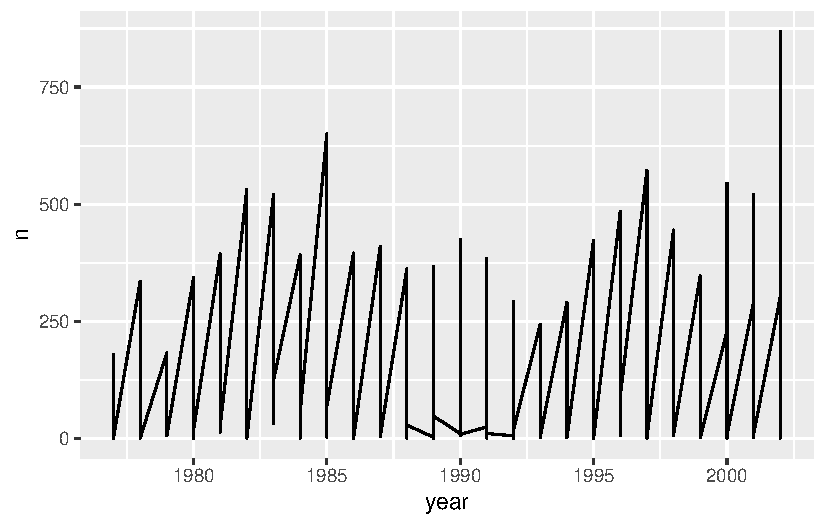
\includegraphics{src/notebooks/r_files/figure-pdf/unnamed-chunk-48-1.pdf}

\begin{Shaded}
\begin{Highlighting}[]
\CommentTok{\# Color for each group}
\NormalTok{surveys\_plot }\OtherTok{\textless{}{-}} \FunctionTok{ggplot}\NormalTok{(}
  \AttributeTok{data =}\NormalTok{ survey\_complete,}
  \AttributeTok{mapping =} \FunctionTok{aes}\NormalTok{(}\AttributeTok{x =}\NormalTok{ weight, }\AttributeTok{y =}\NormalTok{ hindfoot\_length),}
  \AttributeTok{color =}\NormalTok{ species\_id}
\NormalTok{)}
\NormalTok{surveys\_plot}
\end{Highlighting}
\end{Shaded}

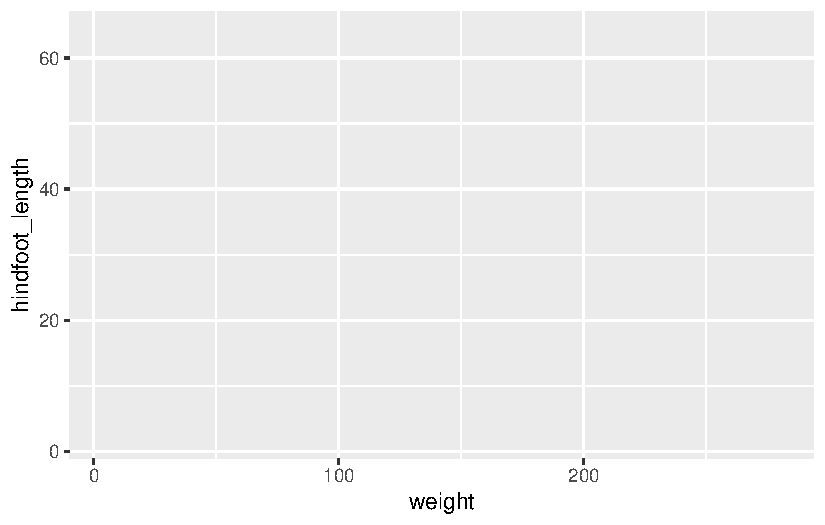
\includegraphics{src/notebooks/r_files/figure-pdf/unnamed-chunk-48-2.pdf}

Step 2: Select the type of the plot

\begin{itemize}
\tightlist
\item
  scatter plot, dot plots, etc. \textgreater{} geom\_point()
\item
  boxplots \textgreater{} geom\_boxplot()
\item
  trend lines, time series, etc. \textgreater{} geom\_line()
\end{itemize}

\subsection{Scatter plot}\label{scatter-plot}

\begin{Shaded}
\begin{Highlighting}[]
\NormalTok{surveys\_plot }\SpecialCharTok{+} \FunctionTok{geom\_point}\NormalTok{()}
\end{Highlighting}
\end{Shaded}

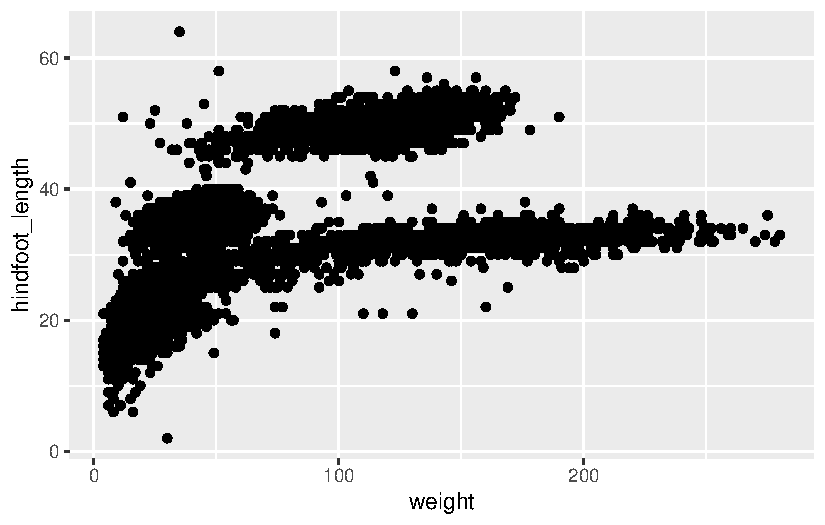
\includegraphics{src/notebooks/r_files/figure-pdf/unnamed-chunk-49-1.pdf}

\begin{Shaded}
\begin{Highlighting}[]
\CommentTok{\# add transparency}
\NormalTok{surveys\_plot }\SpecialCharTok{+} \FunctionTok{geom\_point}\NormalTok{(}\AttributeTok{alpha =} \FloatTok{0.1}\NormalTok{)}
\end{Highlighting}
\end{Shaded}

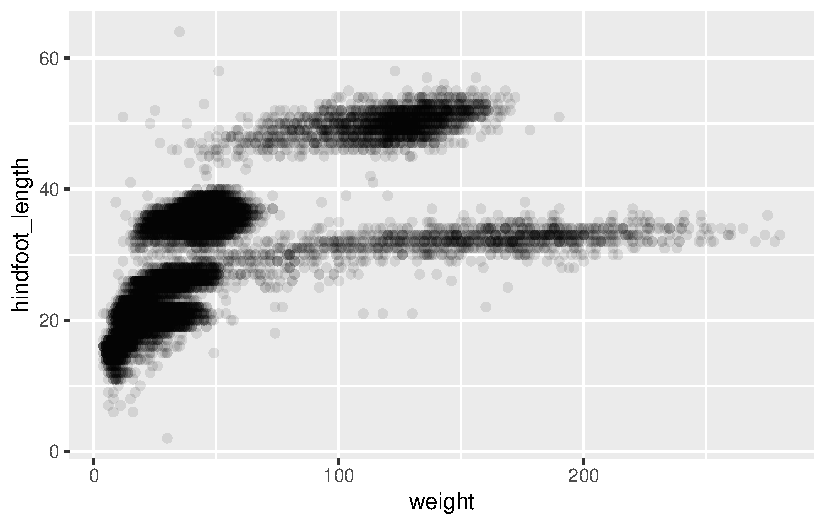
\includegraphics{src/notebooks/r_files/figure-pdf/unnamed-chunk-49-2.pdf}

\begin{Shaded}
\begin{Highlighting}[]
\CommentTok{\# color if not used in binding}
\NormalTok{surveys\_plot }\SpecialCharTok{+} \FunctionTok{geom\_point}\NormalTok{(}\AttributeTok{alpha =} \FloatTok{0.1}\NormalTok{, }\AttributeTok{color =} \StringTok{"black"}\NormalTok{)}
\end{Highlighting}
\end{Shaded}

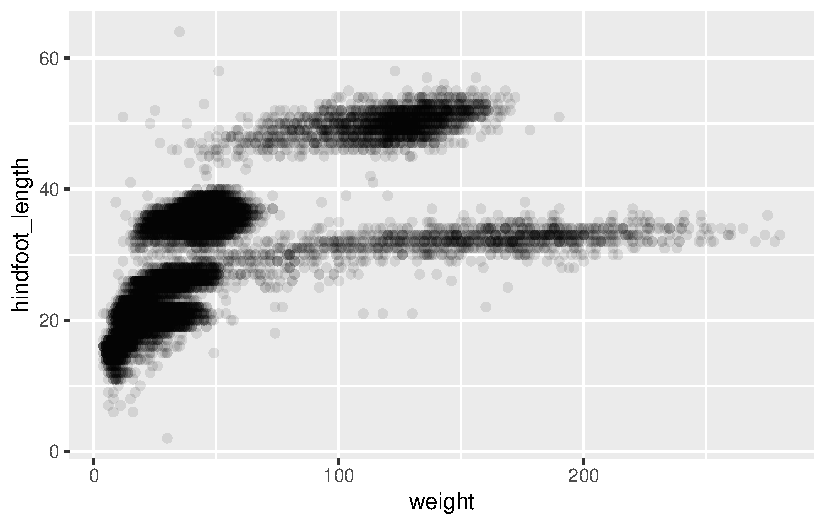
\includegraphics{src/notebooks/r_files/figure-pdf/unnamed-chunk-49-3.pdf}

\begin{Shaded}
\begin{Highlighting}[]
\CommentTok{\# add color if not used in binding}
\NormalTok{surveys\_plot }\SpecialCharTok{+} \FunctionTok{geom\_point}\NormalTok{(}\AttributeTok{alpha =} \FloatTok{0.1}\NormalTok{, }\FunctionTok{aes}\NormalTok{(}\AttributeTok{color =}\NormalTok{ species\_id))}
\end{Highlighting}
\end{Shaded}

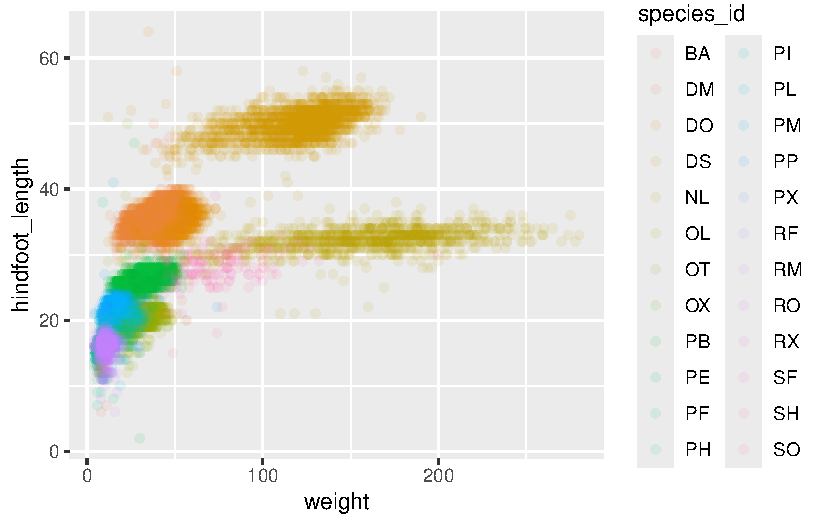
\includegraphics{src/notebooks/r_files/figure-pdf/unnamed-chunk-49-4.pdf}

\begin{Shaded}
\begin{Highlighting}[]
\CommentTok{\# make the color blend by introducing small random variation in points locations}
\CommentTok{\# used when having small data sets}
\NormalTok{surveys\_plot }\SpecialCharTok{+} \FunctionTok{geom\_jitter}\NormalTok{(}\AttributeTok{alpha =} \FloatTok{0.1}\NormalTok{)}
\end{Highlighting}
\end{Shaded}

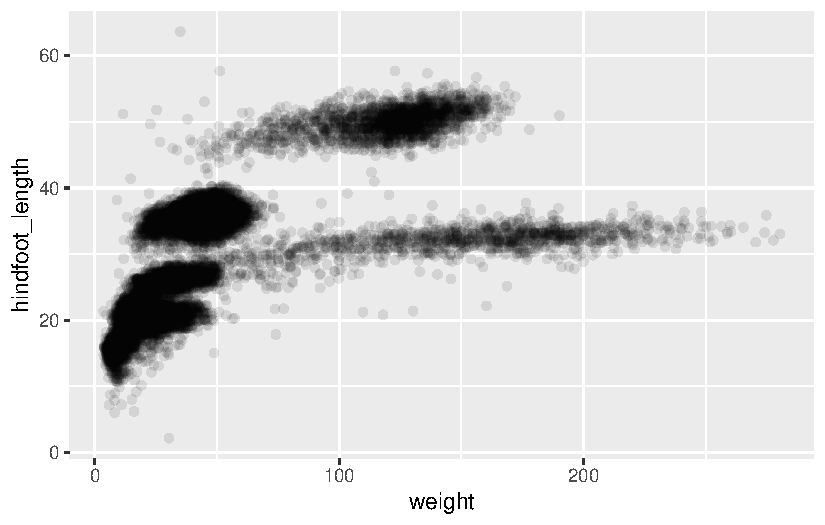
\includegraphics{src/notebooks/r_files/figure-pdf/unnamed-chunk-49-5.pdf}

\subsection{Boxplot}\label{boxplot}

\begin{Shaded}
\begin{Highlighting}[]
\NormalTok{surveys\_plot }\OtherTok{\textless{}{-}} \FunctionTok{ggplot}\NormalTok{(}
  \AttributeTok{data =}\NormalTok{ survey\_complete,}
  \AttributeTok{mapping =} \FunctionTok{aes}\NormalTok{(}\AttributeTok{x =}\NormalTok{ species\_id, }\AttributeTok{y =}\NormalTok{ weight)}
\NormalTok{)}

\NormalTok{surveys\_plot }\SpecialCharTok{+} \FunctionTok{geom\_boxplot}\NormalTok{()}
\end{Highlighting}
\end{Shaded}

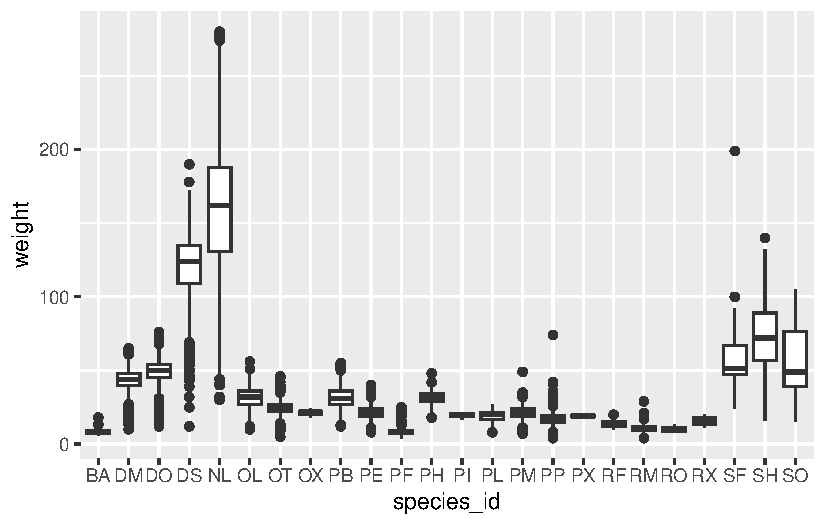
\includegraphics{src/notebooks/r_files/figure-pdf/unnamed-chunk-50-1.pdf}

\begin{Shaded}
\begin{Highlighting}[]
\CommentTok{\# show data}
\NormalTok{surveys\_plot }\SpecialCharTok{+} \FunctionTok{geom\_boxplot}\NormalTok{(}\AttributeTok{alpha =} \FloatTok{0.5}\NormalTok{) }\SpecialCharTok{+}
  \FunctionTok{geom\_jitter}\NormalTok{(}\AttributeTok{alpha =} \FloatTok{0.1}\NormalTok{, }\AttributeTok{color =} \StringTok{"tomato"}\NormalTok{)}
\end{Highlighting}
\end{Shaded}

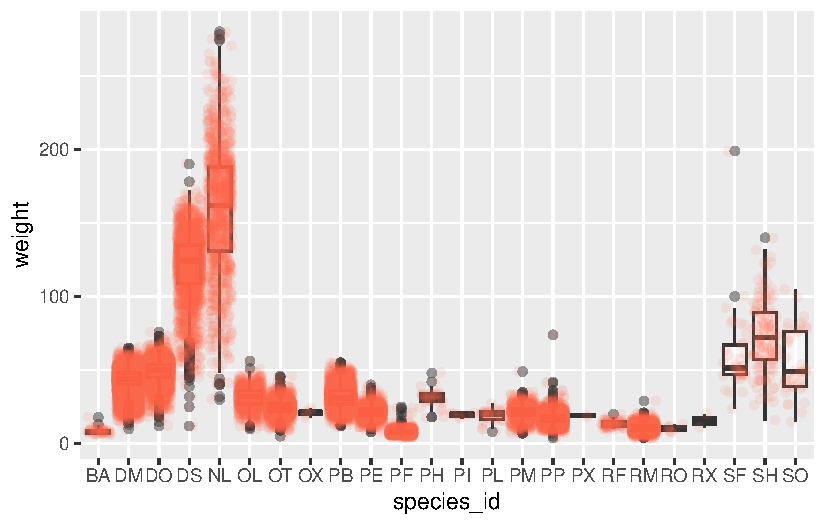
\includegraphics{src/notebooks/r_files/figure-pdf/unnamed-chunk-50-2.pdf}

\begin{Shaded}
\begin{Highlighting}[]
\CommentTok{\# bring boxplot layer in front}
\NormalTok{surveys\_plot }\SpecialCharTok{+} \FunctionTok{geom\_jitter}\NormalTok{(}\AttributeTok{alpha =} \FloatTok{0.1}\NormalTok{, }\AttributeTok{color =} \StringTok{"tomato"}\NormalTok{) }\SpecialCharTok{+}
  \FunctionTok{geom\_boxplot}\NormalTok{(}\AttributeTok{alpha =} \FloatTok{0.7}\NormalTok{)}
\end{Highlighting}
\end{Shaded}

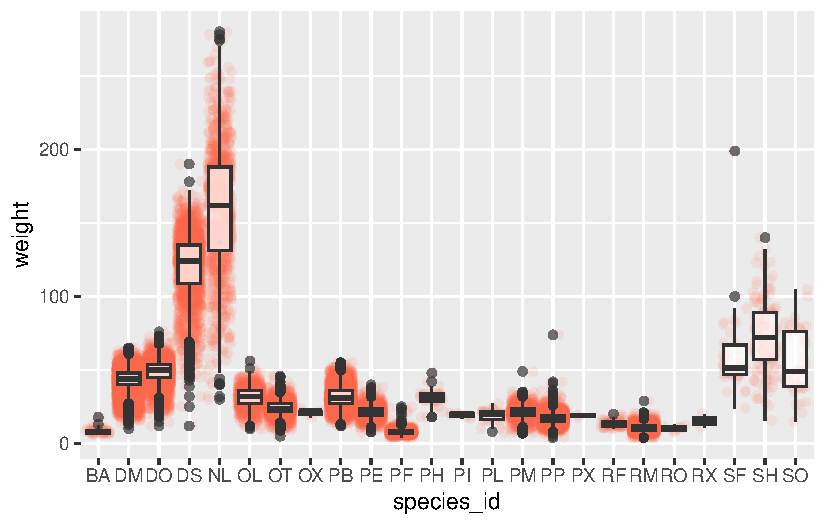
\includegraphics{src/notebooks/r_files/figure-pdf/unnamed-chunk-50-3.pdf}

\subsection{Time series data}\label{time-series-data}

\begin{Shaded}
\begin{Highlighting}[]
\CommentTok{\# create appropriate dataset}
\NormalTok{yearly\_count }\OtherTok{\textless{}{-}}\NormalTok{ survey\_complete }\SpecialCharTok{\%\textgreater{}\%}
  \FunctionTok{count}\NormalTok{(year, species\_id)}

\NormalTok{surveys\_plot }\OtherTok{\textless{}{-}} \FunctionTok{ggplot}\NormalTok{(}
  \AttributeTok{data =}\NormalTok{ yearly\_count,}
  \AttributeTok{mapping =} \FunctionTok{aes}\NormalTok{(}\AttributeTok{x =}\NormalTok{ year, }\AttributeTok{y =}\NormalTok{ n)}
\NormalTok{)}

\NormalTok{surveys\_plot }\SpecialCharTok{+} \FunctionTok{geom\_line}\NormalTok{()}
\end{Highlighting}
\end{Shaded}

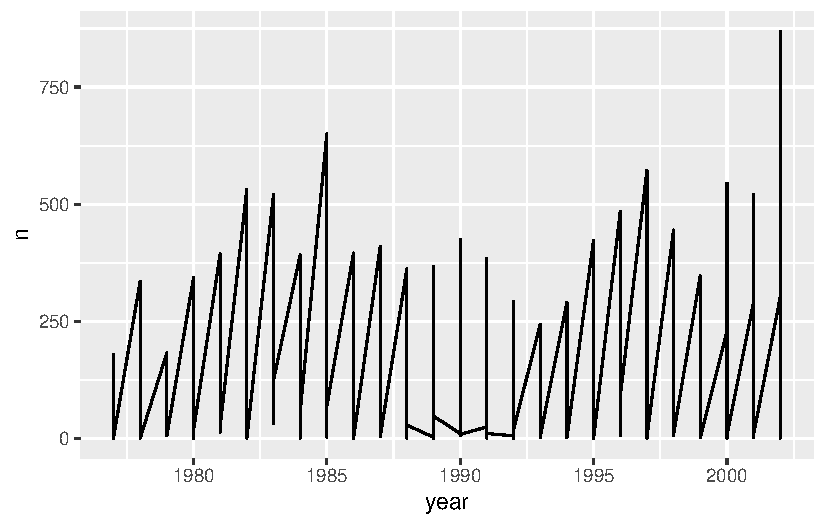
\includegraphics{src/notebooks/r_files/figure-pdf/unnamed-chunk-51-1.pdf}

\begin{Shaded}
\begin{Highlighting}[]
\CommentTok{\# make it more meaningful by breaking it by category}
\NormalTok{surveys\_plot }\SpecialCharTok{+} \FunctionTok{geom\_line}\NormalTok{(}\FunctionTok{aes}\NormalTok{(}\AttributeTok{group =}\NormalTok{ species\_id))}
\end{Highlighting}
\end{Shaded}

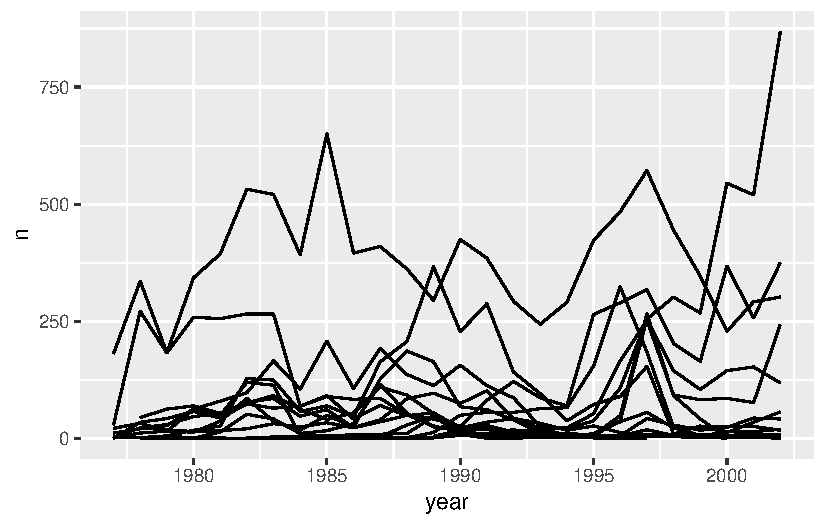
\includegraphics{src/notebooks/r_files/figure-pdf/unnamed-chunk-51-2.pdf}

\begin{Shaded}
\begin{Highlighting}[]
\CommentTok{\# make it more colorful}
\NormalTok{surveys\_plot }\SpecialCharTok{+} \FunctionTok{geom\_line}\NormalTok{(}\FunctionTok{aes}\NormalTok{(}\AttributeTok{color =}\NormalTok{ species\_id))}
\end{Highlighting}
\end{Shaded}

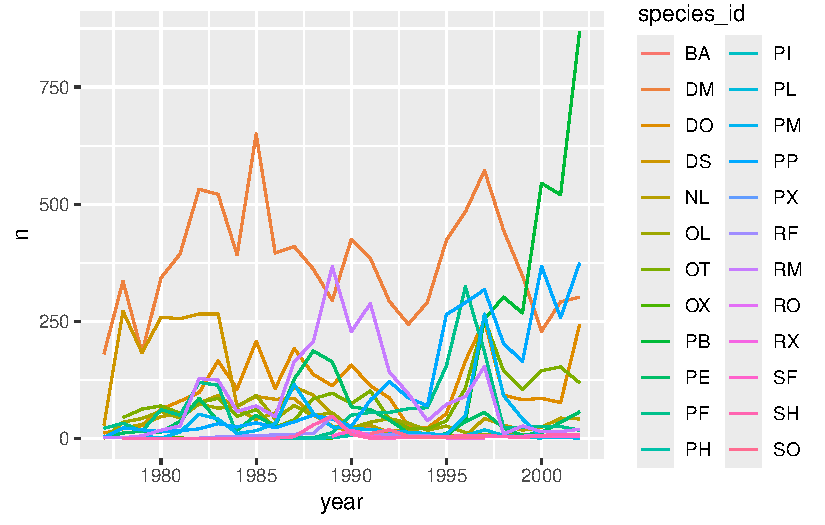
\includegraphics{src/notebooks/r_files/figure-pdf/unnamed-chunk-51-3.pdf}

\begin{Shaded}
\begin{Highlighting}[]
\CommentTok{\# split into multiple plots}
\NormalTok{surveys\_plot }\SpecialCharTok{+} \FunctionTok{geom\_line}\NormalTok{() }\SpecialCharTok{+} \FunctionTok{facet\_wrap}\NormalTok{(}\SpecialCharTok{\textasciitilde{}}\NormalTok{species\_id)}
\end{Highlighting}
\end{Shaded}

\begin{verbatim}
`geom_line()`: Each group consists of only one observation.
i Do you need to adjust the group aesthetic?
\end{verbatim}

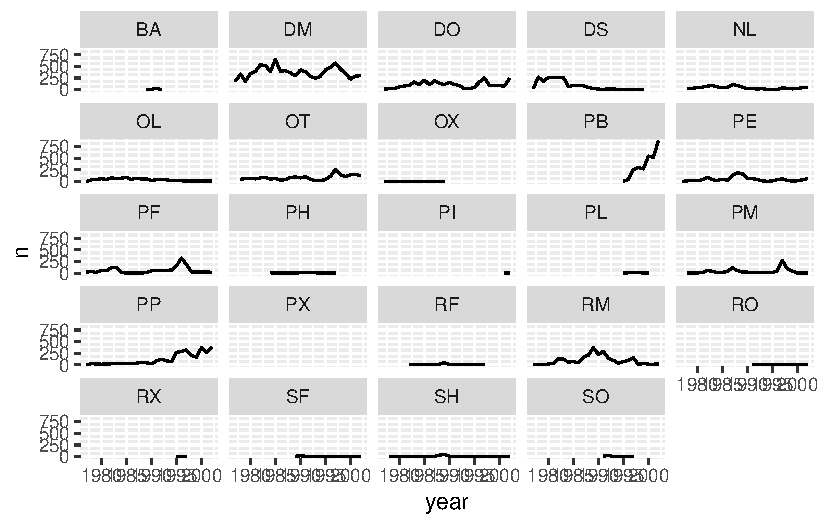
\includegraphics{src/notebooks/r_files/figure-pdf/unnamed-chunk-51-4.pdf}

\begin{Shaded}
\begin{Highlighting}[]
\CommentTok{\# split the line in each plot by sex}
\NormalTok{yearly\_sex\_counts }\OtherTok{\textless{}{-}}\NormalTok{ survey\_complete }\SpecialCharTok{\%\textgreater{}\%}
  \FunctionTok{count}\NormalTok{(year, species\_id, sex)}

\NormalTok{surveys\_plot }\OtherTok{\textless{}{-}} \FunctionTok{ggplot}\NormalTok{(}
  \AttributeTok{data =}\NormalTok{ yearly\_sex\_counts,}
  \AttributeTok{mapping =} \FunctionTok{aes}\NormalTok{(}\AttributeTok{x =}\NormalTok{ year, }\AttributeTok{y =}\NormalTok{ n)}
\NormalTok{)}

\NormalTok{surveys\_plot }\SpecialCharTok{+} \FunctionTok{geom\_line}\NormalTok{(}\FunctionTok{aes}\NormalTok{(}\AttributeTok{color =}\NormalTok{ sex)) }\SpecialCharTok{+}
  \FunctionTok{facet\_wrap}\NormalTok{(}\SpecialCharTok{\textasciitilde{}}\NormalTok{species\_id)}
\end{Highlighting}
\end{Shaded}

\begin{verbatim}
`geom_line()`: Each group consists of only one observation.
i Do you need to adjust the group aesthetic?
\end{verbatim}

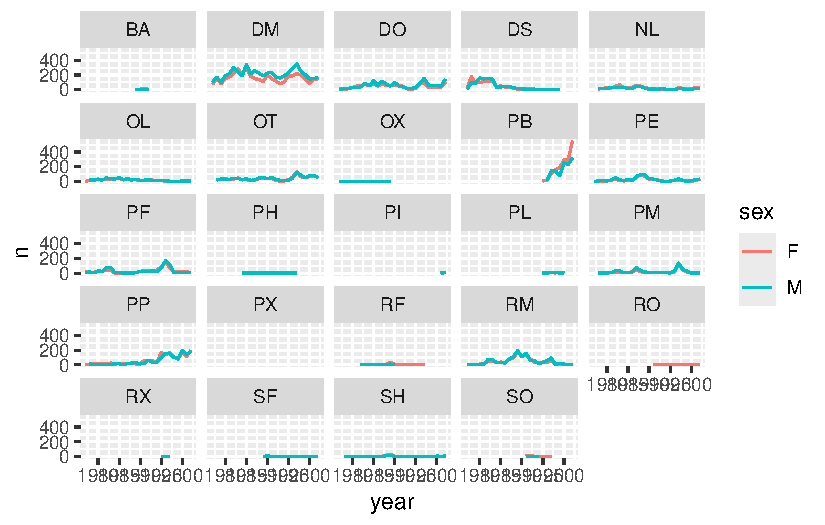
\includegraphics{src/notebooks/r_files/figure-pdf/unnamed-chunk-51-5.pdf}

\begin{Shaded}
\begin{Highlighting}[]
\CommentTok{\# remove background}
\NormalTok{surveys\_plot }\SpecialCharTok{+} \FunctionTok{geom\_line}\NormalTok{(}\FunctionTok{aes}\NormalTok{(}\AttributeTok{color =}\NormalTok{ sex)) }\SpecialCharTok{+}
  \FunctionTok{facet\_wrap}\NormalTok{(}\SpecialCharTok{\textasciitilde{}}\NormalTok{species\_id) }\SpecialCharTok{+}
  \FunctionTok{theme\_bw}\NormalTok{() }\SpecialCharTok{+}
  \FunctionTok{theme}\NormalTok{(}\AttributeTok{panel.grid =} \FunctionTok{element\_blank}\NormalTok{())}
\end{Highlighting}
\end{Shaded}

\begin{verbatim}
`geom_line()`: Each group consists of only one observation.
i Do you need to adjust the group aesthetic?
\end{verbatim}

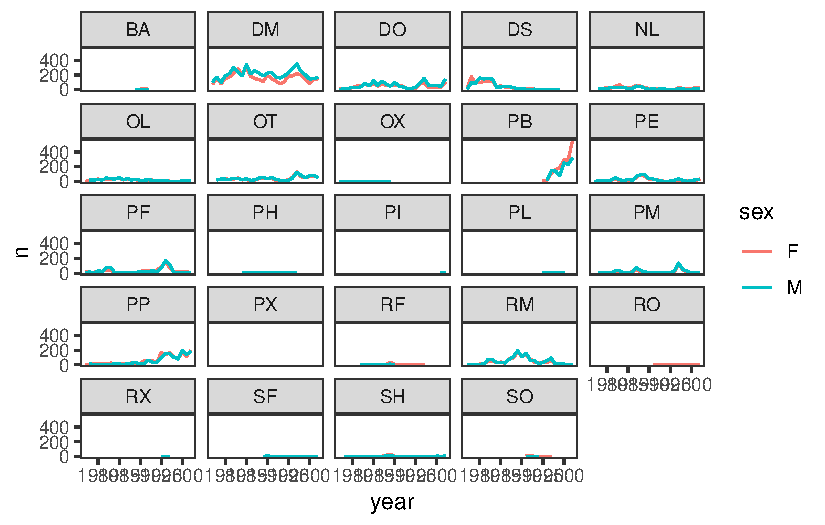
\includegraphics{src/notebooks/r_files/figure-pdf/unnamed-chunk-51-6.pdf}

\section{References}\label{references}

\begin{itemize}
\tightlist
\item
  OU Software Carpentry Workshop (check other workshops
  \href{https://libraries.ou.edu/content/software-and-data-carpentry}{here})

  \begin{itemize}
  \tightlist
  \item
    \href{https://oulib-swc.github.io/2019-05-15-ou-swc/}{Main Tutorial}
  \item
    \href{https://datacarpentry.org/R-ecology-lesson/index.html}{Data
    Carpentry with R}
  \item
    \href{https://swcarpentry.github.io/r-novice-gapminder/}{Software
    Carpentry with R}
  \item
    \href{https://pad.carpentries.org/2019-05-15-ou-swc}{Etherpad}
  \item
    \href{https://docs.google.com/document/d/1aJq_X1uhaNkUj7qdZEzOcpc2Pky7eZPy76yqs0UkfrQ/edit}{Google
    Doc}
  \end{itemize}
\item
  \href{https://rawcdn.githack.com/allisonhorst/data-vis/fc107e063f50ef8695b0a75ed73d74720aca2c65/data_vis_np.html}{Intro
  to ggplot} by \href{https://github.com/allisonhorst}{Allison Horst}
\item
  \href{https://r4ds.had.co.nz/}{R for Data Science book by Garrett
  Grolemund and Hadley Wickham}
\item
  \href{http://journals.plos.org/plosbiology/article?id=10.1371/journal.pbio.1001745}{Best
  Practices for Scientific Computing paper}
\end{itemize}

\chapter{Quarto}\label{quarto}

\section*{Clear Workspace, DON'T
EDIT}\label{clear-workspace-dont-edit-1}
\addcontentsline{toc}{section}{Clear Workspace, DON'T EDIT}

\markright{Clear Workspace, DON'T EDIT}

Always start by clearing the workspace. This ensure objects created in
other files are not used used here.

\begin{Shaded}
\begin{Highlighting}[]
\FunctionTok{rm}\NormalTok{(}\AttributeTok{list =} \FunctionTok{ls}\NormalTok{())}
\end{Highlighting}
\end{Shaded}

\section*{List Used Packages, EDIT}\label{list-used-packages-edit-1}
\addcontentsline{toc}{section}{List Used Packages, EDIT}

\markright{List Used Packages, EDIT}

List all the packages that will be used in chunk below.

\begin{Shaded}
\begin{Highlighting}[]
\NormalTok{packages }\OtherTok{\textless{}{-}} \FunctionTok{c}\NormalTok{()}
\end{Highlighting}
\end{Shaded}

\section*{Load Packages, DON'T EDIT}\label{sec-packages}
\addcontentsline{toc}{section}{Load Packages, DON'T EDIT}

\markright{Load Packages, DON'T EDIT}

\subsection*{Install Missing}\label{install-missing-1}
\addcontentsline{toc}{subsection}{Install Missing}

Any missing package will be installed automatically. This ensure
smoother execution when run by others.

\begin{Shaded}
\begin{Highlighting}[]
\CommentTok{\# Do NOT modify}
\FunctionTok{install.packages}\NormalTok{(}\FunctionTok{setdiff}\NormalTok{(packages, }\FunctionTok{rownames}\NormalTok{(}\FunctionTok{installed.packages}\NormalTok{())))}
\end{Highlighting}
\end{Shaded}

\subsection{Load}\label{load-1}

Load all packages \{-\}

\begin{Shaded}
\begin{Highlighting}[]
\CommentTok{\# Do NOT modify}
\FunctionTok{lapply}\NormalTok{(packages, require, }\AttributeTok{character.only =} \ConstantTok{TRUE}\NormalTok{)}
\end{Highlighting}
\end{Shaded}

\begin{verbatim}
list()
\end{verbatim}

\section{Render \& Review}\label{render-review}

\begin{enumerate}
\def\labelenumi{\arabic{enumi}.}
\tightlist
\item
  VSCode/RStudio -\textgreater{} \emph{Render} button
\item
  Terminal -\textgreater{} \texttt{quarto\ preview}
\item
  Terminal -\textgreater{} \texttt{quarto\ preview\ help}
\end{enumerate}

\section{Render w/o Review}\label{render-wo-review}

\begin{enumerate}
\def\labelenumi{\arabic{enumi}.}
\tightlist
\item
  Terminal -\textgreater{} \texttt{quarto\ render}
\item
  Terminal -\textgreater{} \texttt{quarto\ render\ help}
\end{enumerate}

\section{Import Content}\label{import-content}

To import a document to another use the following shortcodes:

\begin{Shaded}
\begin{Highlighting}[]
\NormalTok{\{\{\textless{} include file.qmd \textgreater{}\}\}}
\end{Highlighting}
\end{Shaded}

\section{References}\label{references-1}

\begin{itemize}
\tightlist
\item
  \href{https://quarto.org/docs/reference/}{Quarto Reference}
\end{itemize}

\chapter{RStudio}\label{rstudio}

\section{Keyboard Shortcuts}\label{keyboard-shortcuts}

\begin{tcolorbox}[enhanced jigsaw, coltitle=black, opacityback=0, colback=white, title=\textcolor{quarto-callout-note-color}{\faInfo}\hspace{0.5em}{Mac Users}, titlerule=0mm, bottomtitle=1mm, arc=.35mm, breakable, colbacktitle=quarto-callout-note-color!10!white, toptitle=1mm, left=2mm, bottomrule=.15mm, opacitybacktitle=0.6, toprule=.15mm, leftrule=.75mm, colframe=quarto-callout-note-color-frame, rightrule=.15mm]

In place of \texttt{Ctrl} in the keyboard shortcuts below, use
\texttt{Cmd}.

\end{tcolorbox}

\begin{tcolorbox}[enhanced jigsaw, coltitle=black, opacityback=0, colback=white, title=\textcolor{quarto-callout-note-color}{\faInfo}\hspace{0.5em}{RStudio Tips}, titlerule=0mm, bottomtitle=1mm, arc=.35mm, breakable, colbacktitle=quarto-callout-note-color!10!white, toptitle=1mm, left=2mm, bottomrule=.15mm, opacitybacktitle=0.6, toprule=.15mm, leftrule=.75mm, colframe=quarto-callout-note-color-frame, rightrule=.15mm]

\href{https://x.com/rstudiotips}{RStudio Tip} on X on how to use RStudio
IDE effectively.

\end{tcolorbox}

Below is a set of helpful keyboard shortcut. The full list can be
reached by clicking Tools -\textgreater{} Keyboard Shortcut Help
(\texttt{Alt+Shift+K}) -\textgreater{} See All Shortcuts

\begin{itemize}
\tightlist
\item
  \texttt{Ctrl+Enter}: execute the code statement at which cursor is
  standing and move the cursor to the beginning of the next statement
\item
  \texttt{Ctrl+Shift+S}: execute the whole R script
\item
  \texttt{Ctrl+Alt+I}: insert new code chunk
\item
  \texttt{Ctrl+Shift+C}: comment/un-comment
\item
  \texttt{Alt-⬆️}: move line up
\item
  \texttt{Alt-⬇️️}: move line down
\item
  \texttt{Ctrl+D}: delete line
\item
  \texttt{Ctrl+Shift+A}: format code
\item
  \texttt{Ctrl+M}: add pipe \texttt{\textbar{}\textgreater{}}
  operator--to change from \texttt{\%\textgreater{}\%}, go to Tools
  -\textgreater{} Global Options\ldots{} -\textgreater{} Code section
  -\textgreater{} Editing tab -\textgreater{} check Use native pipe
  operator, \texttt{\textbar{}\textgreater{}} (requires R 4.1+)
\item
  \texttt{Ctrl++}: increase font size of all windows
\item
  \texttt{Ctrl+-}: decrease font size of all windows
\item
  \texttt{Alt+-} : insert assignment \texttt{\textless{}-}. Notice:

  \begin{itemize}
  \tightlist
  \item
    the inserted assignment it is surrounded by spaces
  \item
    the action happen when the cursor is inside an R chunk or R script
    file
  \end{itemize}
\end{itemize}

\section{Notes}\label{notes}

\begin{itemize}
\tightlist
\item
  \textbf{Working Directory} is the location where R looks for files and
  store files. RStudio showed this location at the top of the
  \emph{console} window. The location can be printed to the console
  using the R command \texttt{getwd()} (get working directory).
\item
  A data-science project typically contains multiple types of data. Each
  type is recommended to be kept in separate folder. These types of data
  are:

  \begin{itemize}
  \tightlist
  \item
    Data
  \item
    Scripts
  \item
    Results
  \item
    Figures
  \end{itemize}
\item
  When creating project using RStudio, a file with the extension
  \texttt{.Rproj} will be created. Clicking this file will automatically
  open the project in RStudio.
\item
  Whenever inside a project, one should only use \emph{relative paths}
  (relative to the working directory, ie, the project home) except for
  file hosted on the internet which require using \emph{absolute paths}.
\end{itemize}

\chapter{Microsoft Windows}\label{microsoft-windows}

\section{CMD Command}\label{cmd-command}

\begin{itemize}
\tightlist
\item
  To know which software has update: run cmd as administrator
  -\textgreater{} type \texttt{winget\ upgrade}. To update all of at
  once, type \texttt{winget\ upgrade\ -\/-all}
\end{itemize}

\part{R for Data Science (2e)}

This section contains replications for the examples used in the
\href{https://r4ds.hadley.nz/}{R for Data Science (2e) book}, one Quarto
file per chapter of the book.

\chapter{Data Visualization}\label{data-visualization}

\section*{Clear Workspace, DON'T
EDIT}\label{clear-workspace-dont-edit-2}
\addcontentsline{toc}{section}{Clear Workspace, DON'T EDIT}

\markright{Clear Workspace, DON'T EDIT}

Always start by clearing the workspace. This ensure objects created in
other files are not used used here.

\begin{Shaded}
\begin{Highlighting}[]
\FunctionTok{rm}\NormalTok{(}\AttributeTok{list =} \FunctionTok{ls}\NormalTok{())}
\end{Highlighting}
\end{Shaded}

\section*{List Used Packages, EDIT}\label{list-used-packages-edit-2}
\addcontentsline{toc}{section}{List Used Packages, EDIT}

\markright{List Used Packages, EDIT}

List all the packages that will be used in chunk below.

\begin{Shaded}
\begin{Highlighting}[]
\NormalTok{packages }\OtherTok{=} \FunctionTok{c}\NormalTok{(}\StringTok{"palmerpenguins"}\NormalTok{, }\StringTok{\textquotesingle{}ggthemes\textquotesingle{}}\NormalTok{, }\StringTok{\textquotesingle{}ggplot2\textquotesingle{}}\NormalTok{, }\StringTok{\textquotesingle{}dplyr\textquotesingle{}}\NormalTok{, }\StringTok{\textquotesingle{}here\textquotesingle{}}\NormalTok{, }\StringTok{\textquotesingle{}knitr\textquotesingle{}}\NormalTok{)}
\end{Highlighting}
\end{Shaded}

\section*{Load Packages, DON'T EDIT}\label{sec-packages}
\addcontentsline{toc}{section}{Load Packages, DON'T EDIT}

\markright{Load Packages, DON'T EDIT}

\subsection*{Install Missing}\label{install-missing-2}
\addcontentsline{toc}{subsection}{Install Missing}

Any missing package will be installed automatically. This ensure
smoother execution when run by others.

\begin{tcolorbox}[enhanced jigsaw, coltitle=black, opacityback=0, colback=white, title=\textcolor{quarto-callout-important-color}{\faExclamation}\hspace{0.5em}{Installing Packages on Other People Machine}, titlerule=0mm, bottomtitle=1mm, arc=.35mm, breakable, colbacktitle=quarto-callout-important-color!10!white, toptitle=1mm, left=2mm, bottomrule=.15mm, opacitybacktitle=0.6, toprule=.15mm, leftrule=.75mm, colframe=quarto-callout-important-color-frame, rightrule=.15mm]

Be aware the people may not like installing packages into their machine
automatically. This might break some of their previous code.

\end{tcolorbox}

\begin{Shaded}
\begin{Highlighting}[]
\CommentTok{\# Do NOT modify}
\FunctionTok{install.packages}\NormalTok{(}\FunctionTok{setdiff}\NormalTok{(packages, }\FunctionTok{rownames}\NormalTok{(}\FunctionTok{installed.packages}\NormalTok{())))}
\end{Highlighting}
\end{Shaded}

\subsection*{Load}\label{load-2}
\addcontentsline{toc}{subsection}{Load}

Load all packages

\begin{Shaded}
\begin{Highlighting}[]
\CommentTok{\# Do NOT modify}
\FunctionTok{lapply}\NormalTok{(packages, require, }\AttributeTok{character.only =} \ConstantTok{TRUE}\NormalTok{)}
\end{Highlighting}
\end{Shaded}

\begin{verbatim}
[[1]]
[1] TRUE

[[2]]
[1] TRUE

[[3]]
[1] TRUE

[[4]]
[1] TRUE

[[5]]
[1] TRUE

[[6]]
[1] TRUE
\end{verbatim}

\section{Introduction}\label{introduction}

This page introduces the plot creation vocabulary step by step

\section{Plot Creation Process}\label{plot-creation-process}

\subsection{Load Dataset}\label{load-dataset}

The \texttt{penguins} dataset from the \texttt{palmerpenguins} package
will be used for plotting. Typically, the package is loaded using the
\texttt{library} function as shown in the code chunk below. However, a
better approach is the one outlined in \textbf{?@sec-packages}.

\begin{Shaded}
\begin{Highlighting}[]
\FunctionTok{library}\NormalTok{(palmerpenguins)}
\end{Highlighting}
\end{Shaded}

Explore the dataset

\begin{Shaded}
\begin{Highlighting}[]
\FunctionTok{help}\NormalTok{(penguins)}
\end{Highlighting}
\end{Shaded}

\begin{verbatim}
Size measurements for adult foraging penguins near Palmer Station,
Antarctica

Description:

     Includes measurements for penguin species, island in Palmer
     Archipelago, size (flipper length, body mass, bill dimensions),
     and sex. This is a subset of 'penguins_raw'.

Usage:

     penguins
     
Format:

     A tibble with 344 rows and 8 variables:

     species a factor denoting penguin species (Adélie, Chinstrap and
          Gentoo)

     island a factor denoting island in Palmer Archipelago, Antarctica
          (Biscoe, Dream or Torgersen)

     bill_length_mm a number denoting bill length (millimeters)

     bill_depth_mm a number denoting bill depth (millimeters)

     flipper_length_mm an integer denoting flipper length (millimeters)

     body_mass_g an integer denoting body mass (grams)

     sex a factor denoting penguin sex (female, male)

     year an integer denoting the study year (2007, 2008, or 2009)

Source:

     Adélie penguins: Palmer Station Antarctica LTER and K. Gorman.
     2020. Structural size measurements and isotopic signatures of
     foraging among adult male and female Adélie penguins (Pygoscelis
     adeliae) nesting along the Palmer Archipelago near Palmer Station,
     2007-2009 ver 5. Environmental Data Initiative. doi:
     10.6073/pasta/98b16d7d563f265cb52372c8ca99e60f (URL:
     https://doi.org/10.6073/pasta/98b16d7d563f265cb52372c8ca99e60f)

     Gentoo penguins: Palmer Station Antarctica LTER and K. Gorman.
     2020. Structural size measurements and isotopic signatures of
     foraging among adult male and female Gentoo penguin (Pygoscelis
     papua) nesting along the Palmer Archipelago near Palmer Station,
     2007-2009 ver 5. Environmental Data Initiative. doi:
     10.6073/pasta/7fca67fb28d56ee2ffa3d9370ebda689 (URL:
     https://doi.org/10.6073/pasta/7fca67fb28d56ee2ffa3d9370ebda689)

     Chinstrap penguins: Palmer Station Antarctica LTER and K. Gorman.
     2020. Structural size measurements and isotopic signatures of
     foraging among adult male and female Chinstrap penguin (Pygoscelis
     antarcticus) nesting along the Palmer Archipelago near Palmer
     Station, 2007-2009 ver 6. Environmental Data Initiative. doi:
     10.6073/pasta/c14dfcfada8ea13a17536e73eb6fbe9e (URL:
     https://doi.org/10.6073/pasta/c14dfcfada8ea13a17536e73eb6fbe9e)

     Originally published in: Gorman KB, Williams TD, Fraser WR (2014)
     Ecological Sexual Dimorphism and Environmental Variability within
     a Community of Antarctic Penguins (Genus Pygoscelis). PLoS ONE
     9(3): e90081. doi:10.1371/journal.pone.0090081
\end{verbatim}

Explore the dataset differently

\begin{Shaded}
\begin{Highlighting}[]
\NormalTok{dplyr}\SpecialCharTok{::}\FunctionTok{glimpse}\NormalTok{(penguins)}
\end{Highlighting}
\end{Shaded}

\begin{verbatim}
Rows: 344
Columns: 8
$ species           <fct> Adelie, Adelie, Adelie, Adelie, Adelie, Adelie, Adel~
$ island            <fct> Torgersen, Torgersen, Torgersen, Torgersen, Torgerse~
$ bill_length_mm    <dbl> 39.1, 39.5, 40.3, NA, 36.7, 39.3, 38.9, 39.2, 34.1, ~
$ bill_depth_mm     <dbl> 18.7, 17.4, 18.0, NA, 19.3, 20.6, 17.8, 19.6, 18.1, ~
$ flipper_length_mm <int> 181, 186, 195, NA, 193, 190, 181, 195, 193, 190, 186~
$ body_mass_g       <int> 3750, 3800, 3250, NA, 3450, 3650, 3625, 4675, 3475, ~
$ sex               <fct> male, female, female, NA, female, male, female, male~
$ year              <int> 2007, 2007, 2007, 2007, 2007, 2007, 2007, 2007, 2007~
\end{verbatim}

\subsection{Load Plotting Package}\label{load-plotting-package}

The \texttt{ggplot2} package will be used for plotting. The package is
typically loaded using the \texttt{library} function as shown in the
code chunk below. However, a better approach is the one outlined in
\textbf{?@sec-packages}.

\begin{Shaded}
\begin{Highlighting}[]
\FunctionTok{library}\NormalTok{(ggplot2)}
\end{Highlighting}
\end{Shaded}

\subsection{\texorpdfstring{Create \texttt{ggplot}
object}{Create ggplot object}}\label{create-ggplot-object}

Create an empty canvas by instantiating a \texttt{ggplot} object using
the \texttt{ggplot()} function.

\begin{Shaded}
\begin{Highlighting}[]
\FunctionTok{ggplot}\NormalTok{()}
\end{Highlighting}
\end{Shaded}


\includegraphics{src/r-for-data-science/01-data-viz_files/figure-pdf/unnamed-chunk-7-1.pdf}

\subsection{Link Dataset}\label{link-dataset}

Link the dataset with the instantiated \texttt{ggplot} object using the
\texttt{data} parameter.

\begin{Shaded}
\begin{Highlighting}[]
\FunctionTok{ggplot}\NormalTok{(}\AttributeTok{data =}\NormalTok{ penguins)}
\end{Highlighting}
\end{Shaded}

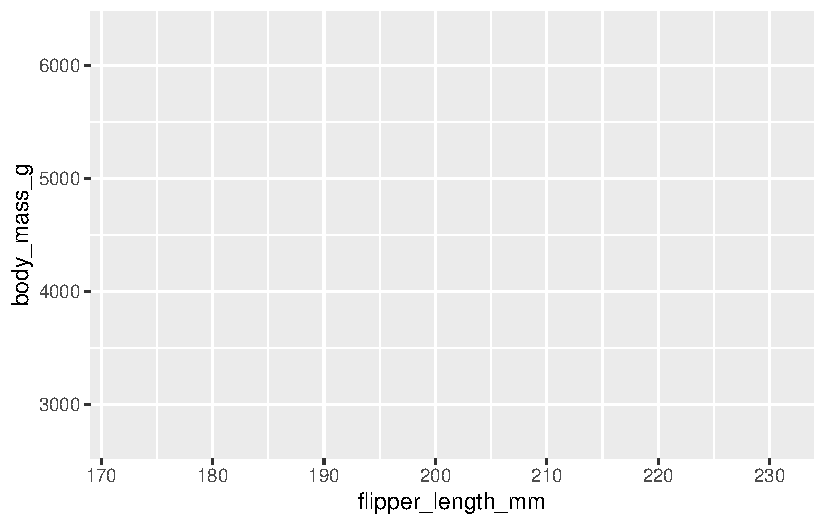
\includegraphics{src/r-for-data-science/01-data-viz_files/figure-pdf/unnamed-chunk-8-1.pdf}

\subsection{Map Two Variables}\label{map-two-variables}

Specify which of the variables in the dataset will be used as the plot
aesthetics (visual properties) using the \texttt{mapping} argument done
via the \texttt{aes()} function.

\begin{Shaded}
\begin{Highlighting}[]
\FunctionTok{ggplot}\NormalTok{(}\AttributeTok{data =}\NormalTok{ penguins,}
       \AttributeTok{mapping =} \FunctionTok{aes}\NormalTok{(}\AttributeTok{x =}\NormalTok{ flipper\_length\_mm, }\AttributeTok{y =}\NormalTok{ body\_mass\_g))}
\end{Highlighting}
\end{Shaded}

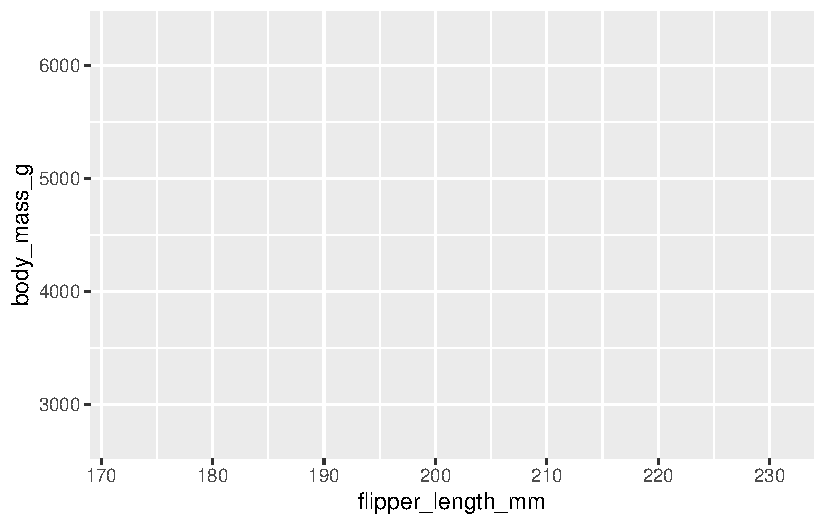
\includegraphics{src/r-for-data-science/01-data-viz_files/figure-pdf/unnamed-chunk-9-1.pdf}

\subsection{Display Data}\label{display-data}

Specify how the data (observations) will be represented geometrically on
the plot, eg, bars, points, or line. The functions starting with
\texttt{geom\_} is used for this purpose. These functions add layer of
the selected geometric object to the plot.

\begin{Shaded}
\begin{Highlighting}[]
\FunctionTok{ggplot}\NormalTok{(}\AttributeTok{data =}\NormalTok{ penguins,}
       \AttributeTok{mapping =} \FunctionTok{aes}\NormalTok{(}\AttributeTok{x =}\NormalTok{ flipper\_length\_mm, }\AttributeTok{y =}\NormalTok{ body\_mass\_g)) }\SpecialCharTok{+}
  \FunctionTok{geom\_point}\NormalTok{()}
\end{Highlighting}
\end{Shaded}

\begin{verbatim}
Warning: Removed 2 rows containing missing values or values outside the scale range
(`geom_point()`).
\end{verbatim}

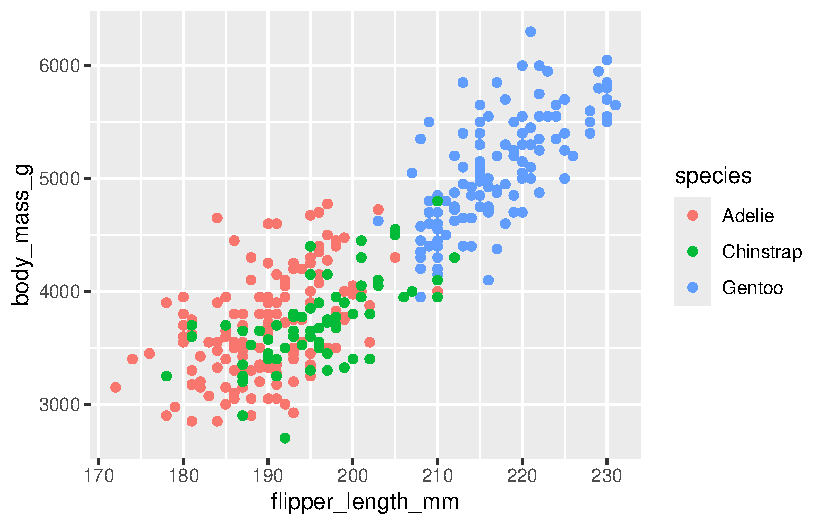
\includegraphics{src/r-for-data-science/01-data-viz_files/figure-pdf/unnamed-chunk-10-1.pdf}

\subsection{Map Third Variables}\label{map-third-variables}

Other variables in the dataset can be linked to plot aesthetics (visual
properties) using the \texttt{mapping} argument done via the
\texttt{aes()} function.

\begin{Shaded}
\begin{Highlighting}[]
\FunctionTok{ggplot}\NormalTok{(}
  \AttributeTok{data =}\NormalTok{ penguins,}
  \AttributeTok{mapping =} \FunctionTok{aes}\NormalTok{(}\AttributeTok{x =}\NormalTok{ flipper\_length\_mm, }\AttributeTok{y =}\NormalTok{ body\_mass\_g, }\AttributeTok{color =}\NormalTok{ species)}
\NormalTok{) }\SpecialCharTok{+}
  \FunctionTok{geom\_point}\NormalTok{()}
\end{Highlighting}
\end{Shaded}

\begin{verbatim}
Warning: Removed 2 rows containing missing values or values outside the scale range
(`geom_point()`).
\end{verbatim}

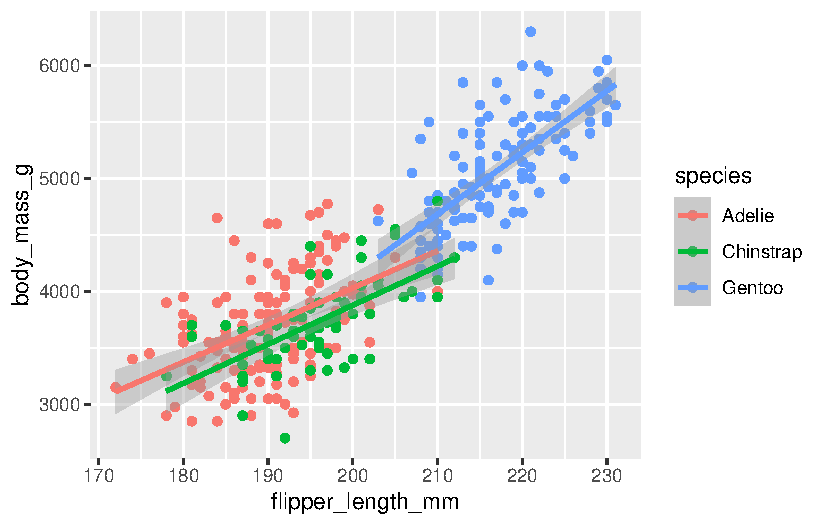
\includegraphics{src/r-for-data-science/01-data-viz_files/figure-pdf/unnamed-chunk-11-1.pdf}

\subsection{Display Three Trendlines}\label{display-three-trendlines}

More geometric representations for the data can be specified using the
functions starting with \texttt{geom\_} which will add layer of the
selected geometric object to the plot.

\begin{Shaded}
\begin{Highlighting}[]
\FunctionTok{ggplot}\NormalTok{(}
  \AttributeTok{data =}\NormalTok{ penguins,}
  \AttributeTok{mapping =} \FunctionTok{aes}\NormalTok{(}\AttributeTok{x =}\NormalTok{ flipper\_length\_mm, }\AttributeTok{y =}\NormalTok{ body\_mass\_g, }\AttributeTok{color =}\NormalTok{ species)}
\NormalTok{) }\SpecialCharTok{+}
  \FunctionTok{geom\_point}\NormalTok{() }\SpecialCharTok{+}
  \FunctionTok{geom\_smooth}\NormalTok{(}\AttributeTok{method =} \StringTok{"lm"}\NormalTok{)}
\end{Highlighting}
\end{Shaded}

\begin{verbatim}
`geom_smooth()` using formula = 'y ~ x'
\end{verbatim}

\begin{verbatim}
Warning: Removed 2 rows containing non-finite outside the scale range
(`stat_smooth()`).
\end{verbatim}

\begin{verbatim}
Warning: Removed 2 rows containing missing values or values outside the scale range
(`geom_point()`).
\end{verbatim}

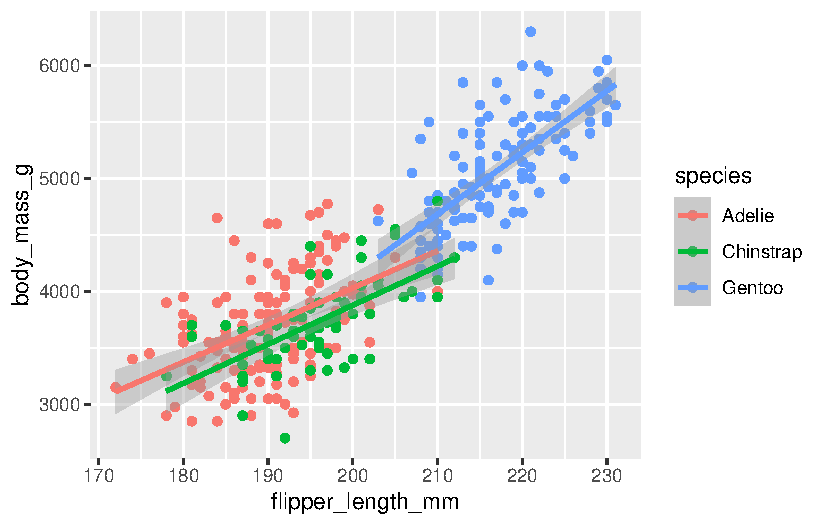
\includegraphics{src/r-for-data-science/01-data-viz_files/figure-pdf/unnamed-chunk-12-1.pdf}

\subsection{Display One Trendline}\label{display-one-trendline}

The aesthetic mapping defined in the \texttt{ggplot()} function is
\emph{global} meaning that all the \texttt{geom\_()} functions inherit
it. However, the aesthetic mapping defined in the \texttt{geom\_()}
functions are \emph{local}, ie, not shared with other \texttt{gemo\_()}
functions.

\begin{Shaded}
\begin{Highlighting}[]
\FunctionTok{ggplot}\NormalTok{(}\AttributeTok{data =}\NormalTok{ penguins,}
       \AttributeTok{mapping =} \FunctionTok{aes}\NormalTok{(}\AttributeTok{x =}\NormalTok{ flipper\_length\_mm, }\AttributeTok{y =}\NormalTok{ body\_mass\_g)) }\SpecialCharTok{+}
  \FunctionTok{geom\_point}\NormalTok{(}\AttributeTok{mapping =} \FunctionTok{aes}\NormalTok{(}\AttributeTok{color =}\NormalTok{ species)) }\SpecialCharTok{+}
  \FunctionTok{geom\_smooth}\NormalTok{(}\AttributeTok{method =} \StringTok{"lm"}\NormalTok{)}
\end{Highlighting}
\end{Shaded}

\begin{verbatim}
`geom_smooth()` using formula = 'y ~ x'
\end{verbatim}

\begin{verbatim}
Warning: Removed 2 rows containing non-finite outside the scale range
(`stat_smooth()`).
\end{verbatim}

\begin{verbatim}
Warning: Removed 2 rows containing missing values or values outside the scale range
(`geom_point()`).
\end{verbatim}

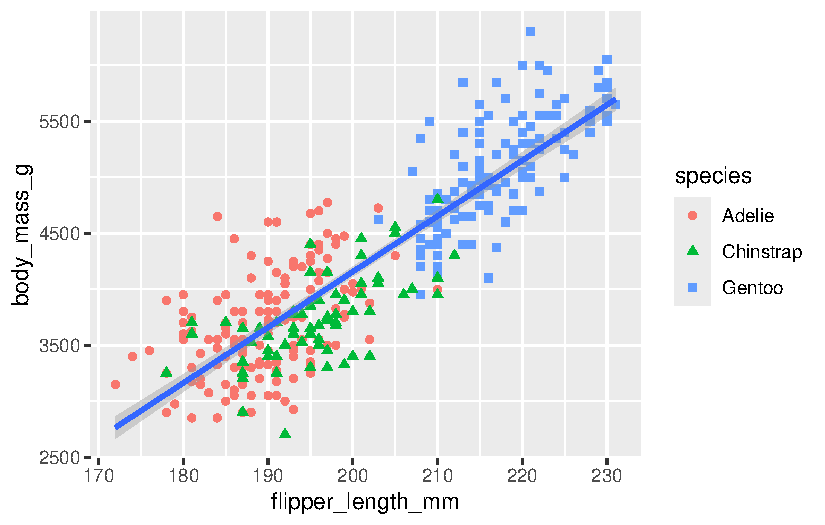
\includegraphics{src/r-for-data-science/01-data-viz_files/figure-pdf/unnamed-chunk-13-1.pdf}

\subsection{Map One Variable Twice}\label{map-one-variable-twice}

We can link the same variable to multiple plot aesthetics (visual
properties) using the \texttt{mapping} parameter done via the
\texttt{aes()} function.

\begin{Shaded}
\begin{Highlighting}[]
\FunctionTok{ggplot}\NormalTok{(}\AttributeTok{data =}\NormalTok{ penguins,}
       \AttributeTok{mapping =} \FunctionTok{aes}\NormalTok{(}\AttributeTok{x =}\NormalTok{ flipper\_length\_mm, }\AttributeTok{y =}\NormalTok{ body\_mass\_g)) }\SpecialCharTok{+}
  \FunctionTok{geom\_point}\NormalTok{(}\AttributeTok{mapping =} \FunctionTok{aes}\NormalTok{(}\AttributeTok{color =}\NormalTok{ species, }\AttributeTok{shape =}\NormalTok{ species)) }\SpecialCharTok{+}
  \FunctionTok{geom\_smooth}\NormalTok{(}\AttributeTok{method =} \StringTok{"lm"}\NormalTok{)}
\end{Highlighting}
\end{Shaded}

\begin{verbatim}
`geom_smooth()` using formula = 'y ~ x'
\end{verbatim}

\begin{verbatim}
Warning: Removed 2 rows containing non-finite outside the scale range
(`stat_smooth()`).
\end{verbatim}

\begin{verbatim}
Warning: Removed 2 rows containing missing values or values outside the scale range
(`geom_point()`).
\end{verbatim}

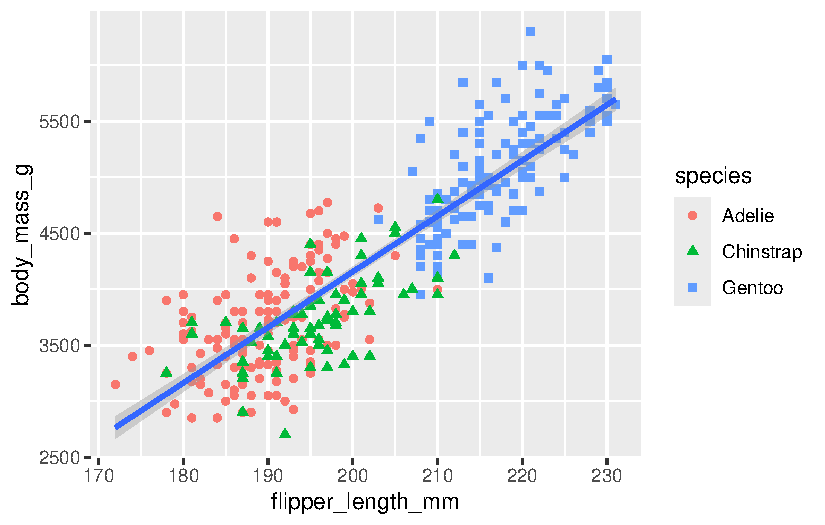
\includegraphics{src/r-for-data-science/01-data-viz_files/figure-pdf/unnamed-chunk-14-1.pdf}

\subsection{Fix Labels}\label{fix-labels}

The \texttt{labs()} function can be used to make the plot more
accessible. The function will add new layer to the plot and the
following items can be added to the layer using the corresponding
parameters

\begin{itemize}
\tightlist
\item
  a title using the \texttt{title} parameter
\item
  a sub-title, if necessary, using the \texttt{subtitle} parameter
\item
  x-axis title using the \texttt{x} parameter
\item
  y-axis title using the \texttt{y} parameter
\item
  data-series label or legend using the \texttt{color} and/or
  \texttt{shape} parameters
\end{itemize}

\begin{Shaded}
\begin{Highlighting}[]
\FunctionTok{ggplot}\NormalTok{(}\AttributeTok{data =}\NormalTok{ penguins,}
       \AttributeTok{mapping =} \FunctionTok{aes}\NormalTok{(}\AttributeTok{x =}\NormalTok{ flipper\_length\_mm, }\AttributeTok{y =}\NormalTok{ body\_mass\_g)) }\SpecialCharTok{+}
  \FunctionTok{geom\_point}\NormalTok{(}\AttributeTok{mapping =} \FunctionTok{aes}\NormalTok{(}\AttributeTok{color =}\NormalTok{ species, }\AttributeTok{shape =}\NormalTok{ species)) }\SpecialCharTok{+}
  \FunctionTok{geom\_smooth}\NormalTok{(}\AttributeTok{method =} \StringTok{"lm"}\NormalTok{) }\SpecialCharTok{+}
  \FunctionTok{labs}\NormalTok{(}
    \AttributeTok{title =} \StringTok{\textquotesingle{}Palmer Three Species Penguins\textquotesingle{}}\NormalTok{,}
    \AttributeTok{subtitle =} \StringTok{\textquotesingle{}The flipper length has a moderattly strong positive linear relationship with the body mass\textquotesingle{}}\NormalTok{,}
    \AttributeTok{x =} \StringTok{\textquotesingle{}Fliper length (mm)\textquotesingle{}}\NormalTok{,}
    \AttributeTok{y =} \StringTok{\textquotesingle{}Body mass (g)\textquotesingle{}}\NormalTok{,}
    \AttributeTok{shape =} \StringTok{\textquotesingle{}Species\textquotesingle{}}\NormalTok{,}
    \AttributeTok{color =} \StringTok{\textquotesingle{}Species\textquotesingle{}}
\NormalTok{  )}
\end{Highlighting}
\end{Shaded}

\begin{verbatim}
`geom_smooth()` using formula = 'y ~ x'
\end{verbatim}

\begin{verbatim}
Warning: Removed 2 rows containing non-finite outside the scale range
(`stat_smooth()`).
\end{verbatim}

\begin{verbatim}
Warning: Removed 2 rows containing missing values or values outside the scale range
(`geom_point()`).
\end{verbatim}

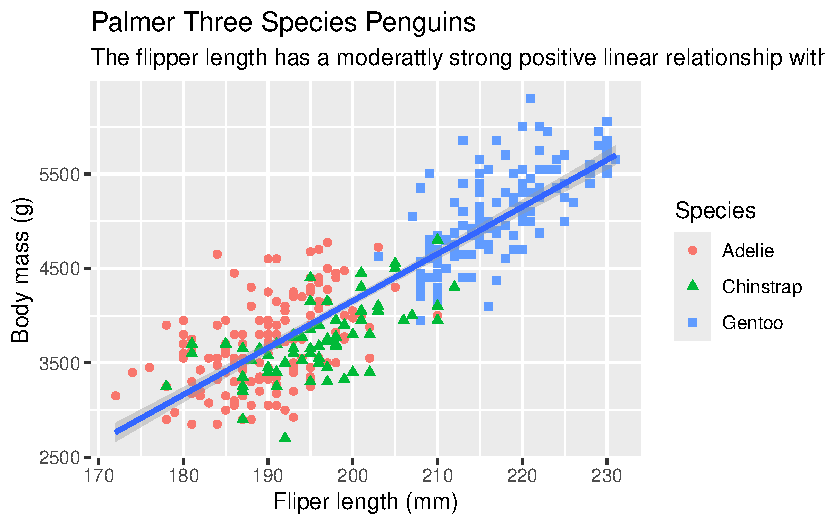
\includegraphics{src/r-for-data-science/01-data-viz_files/figure-pdf/unnamed-chunk-15-1.pdf}

Other types of texts can be added using other functions. The other types
of texts are:

\begin{itemize}
\tightlist
\item
  x-axis label
\item
  y-axis label
\item
  data labels, if necessary
\item
  annotation for interesting or important data, if exist
\end{itemize}

\subsection{Ensure Color-blind Safe}\label{ensure-color-blind-safe}

Make the plot more color-blind safe by using the
\texttt{scale\_color\_colorblind()} function from the \texttt{ggthemes}
package which will add new layer to the plot.

\begin{Shaded}
\begin{Highlighting}[]
\FunctionTok{ggplot}\NormalTok{(}\AttributeTok{data =}\NormalTok{ penguins,}
       \AttributeTok{mapping =} \FunctionTok{aes}\NormalTok{(}\AttributeTok{x =}\NormalTok{ flipper\_length\_mm, }\AttributeTok{y =}\NormalTok{ body\_mass\_g)) }\SpecialCharTok{+}
  \FunctionTok{geom\_point}\NormalTok{(}\AttributeTok{mapping =} \FunctionTok{aes}\NormalTok{(}\AttributeTok{color =}\NormalTok{ species, }\AttributeTok{shape =}\NormalTok{ species)) }\SpecialCharTok{+}
  \FunctionTok{geom\_smooth}\NormalTok{(}\AttributeTok{method =} \StringTok{"lm"}\NormalTok{) }\SpecialCharTok{+}
  \FunctionTok{labs}\NormalTok{(}
    \AttributeTok{title =} \StringTok{\textquotesingle{}Palmer Three Species Penguins\textquotesingle{}}\NormalTok{,}
    \AttributeTok{subtitle =} \StringTok{\textquotesingle{}The flipper length has a moderattly strong positive linear relationship with the body mass\textquotesingle{}}\NormalTok{,}
    \AttributeTok{x =} \StringTok{\textquotesingle{}Fliper length (mm)\textquotesingle{}}\NormalTok{,}
    \AttributeTok{y =} \StringTok{\textquotesingle{}Body mass (g)\textquotesingle{}}\NormalTok{,}
    \AttributeTok{shape =} \StringTok{\textquotesingle{}Species\textquotesingle{}}\NormalTok{,}
    \AttributeTok{color =} \StringTok{\textquotesingle{}Species\textquotesingle{}}
\NormalTok{  ) }\SpecialCharTok{+}
  \FunctionTok{scale\_color\_colorblind}\NormalTok{()}
\end{Highlighting}
\end{Shaded}

\begin{verbatim}
`geom_smooth()` using formula = 'y ~ x'
\end{verbatim}

\begin{verbatim}
Warning: Removed 2 rows containing non-finite outside the scale range
(`stat_smooth()`).
\end{verbatim}

\begin{verbatim}
Warning: Removed 2 rows containing missing values or values outside the scale range
(`geom_point()`).
\end{verbatim}

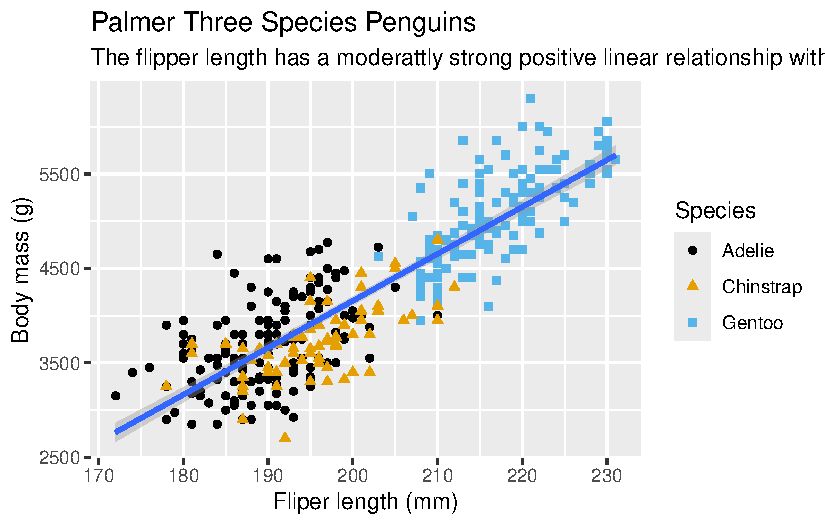
\includegraphics{src/r-for-data-science/01-data-viz_files/figure-pdf/unnamed-chunk-16-1.pdf}

\subsection{Can Call Implicitly}\label{can-call-implicitly}

The first one or two arguments of functions are so important that
scientists should know them by heart. Hence, to save some typing, the
name of these arguments are usually omitted and only the values assigned
to them are kept, ie, the names becomes implicit and no more explicit.
Hence, the above call can be written as follows--the arguments
\texttt{data} and \texttt{mapping} were omitted.

\begin{Shaded}
\begin{Highlighting}[]
\FunctionTok{ggplot}\NormalTok{(penguins, }\FunctionTok{aes}\NormalTok{(}\AttributeTok{x =}\NormalTok{ flipper\_length\_mm, }\AttributeTok{y =}\NormalTok{ body\_mass\_g)) }\SpecialCharTok{+}
  \FunctionTok{geom\_point}\NormalTok{(}\FunctionTok{aes}\NormalTok{(}\AttributeTok{color =}\NormalTok{ species, }\AttributeTok{shape =}\NormalTok{ species)) }\SpecialCharTok{+}
  \FunctionTok{geom\_smooth}\NormalTok{(}\AttributeTok{method =} \StringTok{"lm"}\NormalTok{) }\SpecialCharTok{+}
  \FunctionTok{labs}\NormalTok{(}
    \AttributeTok{title =} \StringTok{\textquotesingle{}Palmer Three Species Penguins\textquotesingle{}}\NormalTok{,}
    \AttributeTok{subtitle =} \StringTok{\textquotesingle{}The flipper length has a moderattly strong positive linear relationship with the body mass\textquotesingle{}}\NormalTok{,}
    \AttributeTok{x =} \StringTok{\textquotesingle{}Fliper length (mm)\textquotesingle{}}\NormalTok{,}
    \AttributeTok{y =} \StringTok{\textquotesingle{}Body mass (g)\textquotesingle{}}\NormalTok{,}
    \AttributeTok{shape =} \StringTok{\textquotesingle{}Species\textquotesingle{}}\NormalTok{,}
    \AttributeTok{color =} \StringTok{\textquotesingle{}Species\textquotesingle{}}
\NormalTok{  ) }\SpecialCharTok{+}
  \FunctionTok{scale\_color\_colorblind}\NormalTok{()}
\end{Highlighting}
\end{Shaded}

\begin{verbatim}
`geom_smooth()` using formula = 'y ~ x'
\end{verbatim}

\begin{verbatim}
Warning: Removed 2 rows containing non-finite outside the scale range
(`stat_smooth()`).
\end{verbatim}

\begin{verbatim}
Warning: Removed 2 rows containing missing values or values outside the scale range
(`geom_point()`).
\end{verbatim}

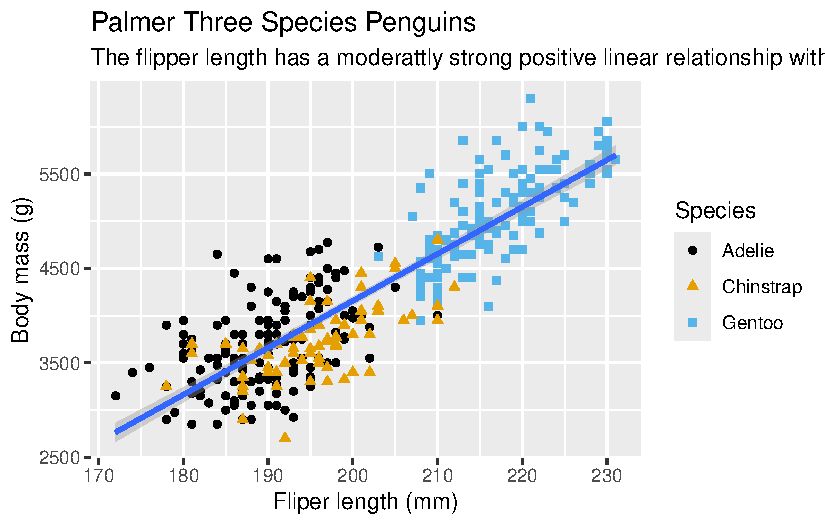
\includegraphics{src/r-for-data-science/01-data-viz_files/figure-pdf/unnamed-chunk-17-1.pdf}

\subsection{Use Pipe Operator}\label{use-pipe-operator}

The pipe operator \texttt{\textbackslash{}\textgreater{}} (shortcut:
\texttt{Ctrl+M}) can be used to make the code tidy. The above code can
be re-written as follow--notice the dataset was pulled before the call
to the \texttt{ggplot()} function.

\begin{Shaded}
\begin{Highlighting}[]
\NormalTok{penguins }\SpecialCharTok{|\textgreater{}}
  \FunctionTok{ggplot}\NormalTok{(}\FunctionTok{aes}\NormalTok{(}\AttributeTok{x =}\NormalTok{ flipper\_length\_mm, }\AttributeTok{y =}\NormalTok{ body\_mass\_g)) }\SpecialCharTok{+}
  \FunctionTok{geom\_point}\NormalTok{(}\FunctionTok{aes}\NormalTok{(}\AttributeTok{color =}\NormalTok{ species, }\AttributeTok{shape =}\NormalTok{ species)) }\SpecialCharTok{+}
  \FunctionTok{geom\_smooth}\NormalTok{(}\AttributeTok{method =} \StringTok{"lm"}\NormalTok{) }\SpecialCharTok{+}
  \FunctionTok{labs}\NormalTok{(}
    \AttributeTok{title =} \StringTok{\textquotesingle{}Palmer Three Species Penguins\textquotesingle{}}\NormalTok{,}
    \AttributeTok{subtitle =} \StringTok{\textquotesingle{}The flipper length has a moderattly strong positive linear relationship with the body mass\textquotesingle{}}\NormalTok{,}
    \AttributeTok{x =} \StringTok{\textquotesingle{}Fliper length (mm)\textquotesingle{}}\NormalTok{,}
    \AttributeTok{y =} \StringTok{\textquotesingle{}Body mass (g)\textquotesingle{}}\NormalTok{,}
    \AttributeTok{shape =} \StringTok{\textquotesingle{}Species\textquotesingle{}}\NormalTok{,}
    \AttributeTok{color =} \StringTok{\textquotesingle{}Species\textquotesingle{}}
\NormalTok{  ) }\SpecialCharTok{+}
  \FunctionTok{scale\_color\_colorblind}\NormalTok{()}
\end{Highlighting}
\end{Shaded}

\begin{verbatim}
`geom_smooth()` using formula = 'y ~ x'
\end{verbatim}

\begin{verbatim}
Warning: Removed 2 rows containing non-finite outside the scale range
(`stat_smooth()`).
\end{verbatim}

\begin{verbatim}
Warning: Removed 2 rows containing missing values or values outside the scale range
(`geom_point()`).
\end{verbatim}

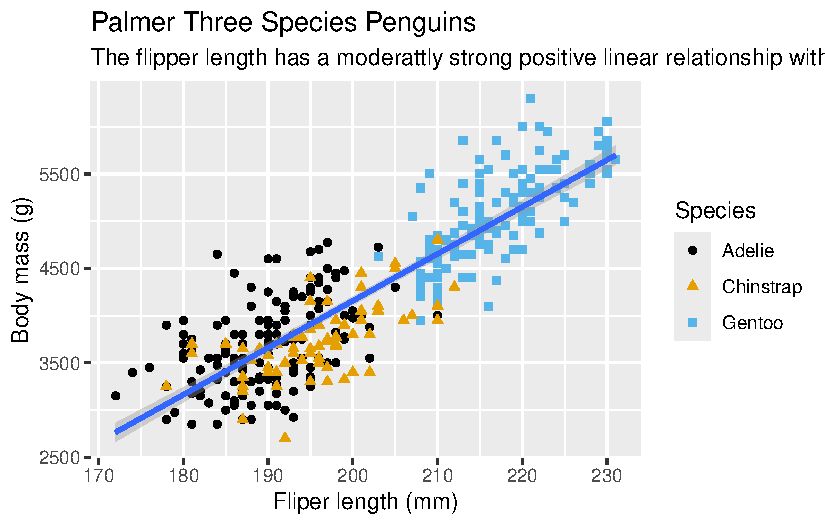
\includegraphics{src/r-for-data-science/01-data-viz_files/figure-pdf/unnamed-chunk-18-1.pdf}

\section{Visualizing Distribution}\label{visualizing-distribution}

\subsection{Categorical Variables}\label{categorical-variables}

Plot options to visualize how a categorical variable is distributed:

\begin{itemize}
\tightlist
\item
  bar chart, if the counts are not computed, using \texttt{gemo\_bar()}
  function
\item
  column chart, if the counts are computed, \texttt{gemo\_col()}
  function
\end{itemize}

\subsection{Numerical Variables}\label{numerical-variables}

Plot options to visualize how a numerical (discrete or continuous)
variable is distributed:

\begin{itemize}
\tightlist
\item
  histogram, using \texttt{geom\_histogram()} function
\end{itemize}

\begin{tcolorbox}[enhanced jigsaw, coltitle=black, opacityback=0, colback=white, title=\textcolor{quarto-callout-note-color}{\faInfo}\hspace{0.5em}{Histogram Bin Width}, titlerule=0mm, bottomtitle=1mm, arc=.35mm, breakable, colbacktitle=quarto-callout-note-color!10!white, toptitle=1mm, left=2mm, bottomrule=.15mm, opacitybacktitle=0.6, toprule=.15mm, leftrule=.75mm, colframe=quarto-callout-note-color-frame, rightrule=.15mm]

The bin width of the histogram is in the unit of the variable mapped to
the plot \texttt{x} (or \texttt{y}) aesthetic (visual property)

\end{tcolorbox}

\begin{itemize}
\tightlist
\item
  density plot, using \texttt{geom\_density()} function
\item
  boxplot, using \texttt{geom\_boplot()} function
\end{itemize}

\begin{tcolorbox}[enhanced jigsaw, coltitle=black, opacityback=0, colback=white, title=\textcolor{quarto-callout-note-color}{\faInfo}\hspace{0.5em}{Boxplot Components}, titlerule=0mm, bottomtitle=1mm, arc=.35mm, breakable, colbacktitle=quarto-callout-note-color!10!white, toptitle=1mm, left=2mm, bottomrule=.15mm, opacitybacktitle=0.6, toprule=.15mm, leftrule=.75mm, colframe=quarto-callout-note-color-frame, rightrule=.15mm]

As described beautifully in
\href{https://r4ds.hadley.nz/data-visualize\#visualizing-relationships}{R4DS},
a boxplot consists of:

\begin{enumerate}
\def\labelenumi{\arabic{enumi}.}
\item
  A box that describes the range of the middle half of the data, a
  distance known as the interquartile range (IQR), stretching from the
  25th percentile of the distribution to the 75th percentile.
\item
  A line in the middle of the box displaying the median, ie, the 50th
  percentile, of the distribution.
\item
  The box and the line give sense of the spread of the distribution and
  whether or not the distribution is symmetric about the median or
  skewed to one side
\item
  Visual points that display the observations that fall more than 1.5
  time the IQR from either edge of the box. These outlying points (hence
  called outliers) are unusual so are plotted individually
\item
  A whisker that extend from each end of the box and goes to the
  farthest non-outlier point in the distribution
\end{enumerate}

Below is the diagram from
\href{https://r4ds.hadley.nz/data-visualize\#visualizing-relationships}{R4DS}
showing the above components and how the boxpot is created.

\begin{figure}[H]

\centering{

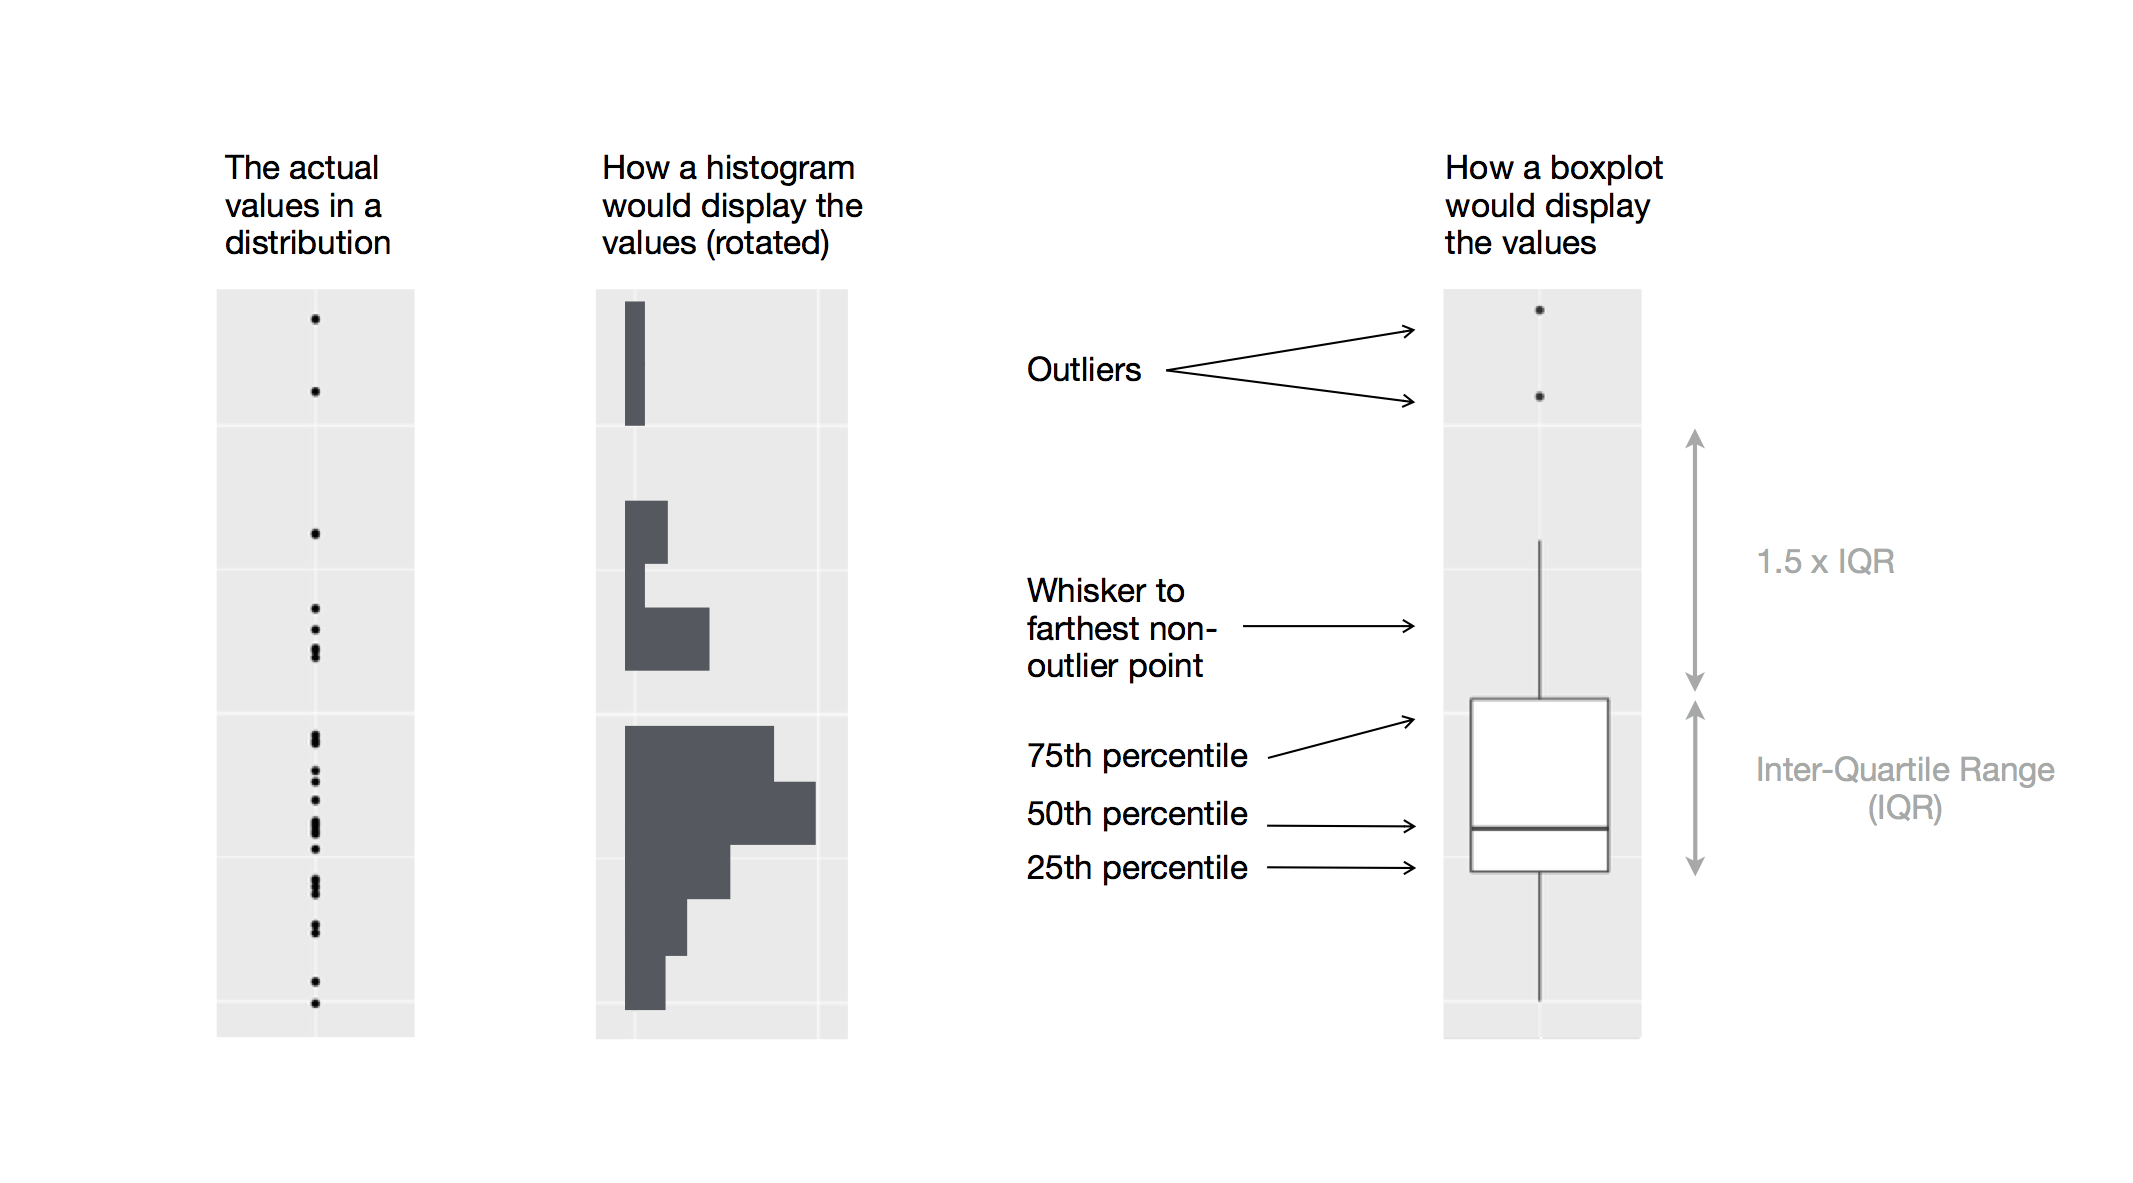
\includegraphics{src/r-for-data-science/../../images/EDA-boxplot.png}

}

\caption{\label{fig-boxplot}Boxplot Components (taken from
\href{https://r4ds.hadley.nz/data-visualize\#visualizing-relationships}{R4DS})}

\end{figure}%

\end{tcolorbox}

\section{Visualizing Relationships}\label{visualizing-relationships}

\subsection{One Categorical + One
Numerical}\label{one-categorical-one-numerical}

For each category of the categorical variable, We can use any of the
plot options mentioned above for the numerical variables

\subsection{Two Categoricals}\label{two-categoricals}

Each category of one of the categorical variables will be placed on the
x-axis (or the y-axis) by mapping it to the plot \texttt{x} (or
\texttt{y}) aesthetic (visual property) of the \texttt{geom\_bar()} and
the distribution of the categories of the other categorical variables by
mapping it to the plot \texttt{fill} aesthetic (visual property). The
second variable can be shown as:

\begin{itemize}
\tightlist
\item
  pure counts (stacked bar chart), or
\item
  percentages (percent stack bar chart) by setting the \texttt{position}
  attribute of the \texttt{geom\_bar()} to \texttt{fill}.
\end{itemize}

\subsection{Two Numerical}\label{two-numerical}

Plot options to show the relationship between two numerical variables
are:

\begin{itemize}
\tightlist
\item
  Scatter plot using the \texttt{geom\_point()} function
\item
  trend line using \texttt{geom\_smooth()} function
\item
  line graph using \texttt{geom\_line()} function if one of the
  variables is monotonic, eg, time or date.
\end{itemize}

\subsection{Three or More Variables}\label{three-or-more-variables}

To visualize 3+ variables, We can either

\begin{itemize}
\tightlist
\item
  map variables to other aesthetics of the plot, eg, \emph{color},
  \emph{size}, and \emph{shape}
\item
  split plot into facets, subplots that each display one subset of the
  data, based on a categorical variable using \texttt{facet\_wrap()}
  function where its first argument is a formula created using
  \texttt{\textasciitilde{}} followed by a (categorical) variable name.
\end{itemize}

\chapter{Workflow: Basics}\label{workflow-basics}

\section*{Clear Workspace, DON'T
EDIT}\label{clear-workspace-dont-edit-3}
\addcontentsline{toc}{section}{Clear Workspace, DON'T EDIT}

\markright{Clear Workspace, DON'T EDIT}

Always start by clearing the workspace. This ensure objects created in
other files are not used used here.

\begin{Shaded}
\begin{Highlighting}[]
\FunctionTok{rm}\NormalTok{(}\AttributeTok{list =} \FunctionTok{ls}\NormalTok{())}
\end{Highlighting}
\end{Shaded}

\section*{List Used Packages, EDIT}\label{list-used-packages-edit-3}
\addcontentsline{toc}{section}{List Used Packages, EDIT}

\markright{List Used Packages, EDIT}

List all the packages that will be used in chunk below.

\begin{Shaded}
\begin{Highlighting}[]
\NormalTok{packages }\OtherTok{\textless{}{-}} \FunctionTok{c}\NormalTok{()}
\end{Highlighting}
\end{Shaded}

\section*{Load Packages, DON'T EDIT}\label{sec-packages}
\addcontentsline{toc}{section}{Load Packages, DON'T EDIT}

\markright{Load Packages, DON'T EDIT}

\subsection*{Install Missing}\label{install-missing-3}
\addcontentsline{toc}{subsection}{Install Missing}

Any missing package will be installed automatically. This ensure
smoother execution when run by others.

\begin{tcolorbox}[enhanced jigsaw, coltitle=black, opacityback=0, colback=white, title=\textcolor{quarto-callout-important-color}{\faExclamation}\hspace{0.5em}{Installing Packages on Other People Machine}, titlerule=0mm, bottomtitle=1mm, arc=.35mm, breakable, colbacktitle=quarto-callout-important-color!10!white, toptitle=1mm, left=2mm, bottomrule=.15mm, opacitybacktitle=0.6, toprule=.15mm, leftrule=.75mm, colframe=quarto-callout-important-color-frame, rightrule=.15mm]

Be aware the people may not like installing packages into their machine
automatically. This might break some of their previous code.

\end{tcolorbox}

\begin{Shaded}
\begin{Highlighting}[]
\CommentTok{\# Do NOT modify}
\FunctionTok{install.packages}\NormalTok{(}\FunctionTok{setdiff}\NormalTok{(packages, }\FunctionTok{rownames}\NormalTok{(}\FunctionTok{installed.packages}\NormalTok{())))}
\end{Highlighting}
\end{Shaded}

\subsection*{Load}\label{load-3}
\addcontentsline{toc}{subsection}{Load}

Load all packages

\begin{Shaded}
\begin{Highlighting}[]
\CommentTok{\# Do NOT modify}
\FunctionTok{lapply}\NormalTok{(packages, require, }\AttributeTok{character.only =} \ConstantTok{TRUE}\NormalTok{)}
\end{Highlighting}
\end{Shaded}

\begin{verbatim}
list()
\end{verbatim}

\section{Introduction}\label{introduction-1}

This page covers basic concepts when working with R. I took note for
those that were new to me or found useful to remind myself with.

\section{Comments}\label{comments}

Use comments to explain the \emph{why} of your code, eg, you changed the
default value of a parameter of a function from say \texttt{.2} to
\texttt{.9}, why?

\section{Nameing Objects Rules}\label{nameing-objects-rules}

\begin{itemize}
\tightlist
\item
  Allowed characters when naming objects

  \begin{itemize}
  \tightlist
  \item
    letters
  \item
    numbers
  \item
    \texttt{\_}
  \item
    \texttt{.}
  \end{itemize}
\item
  All names must start with a letter
\item
  R is case-sensitive, ie, \texttt{var}, \texttt{Var}, and \texttt{VAR}
  are different names
\end{itemize}

\chapter{Data Transformation}\label{data-transformation}

\section*{Clear Workspace, DON'T
EDIT}\label{clear-workspace-dont-edit-4}
\addcontentsline{toc}{section}{Clear Workspace, DON'T EDIT}

\markright{Clear Workspace, DON'T EDIT}

Always start by clearing the workspace. This ensure objects created in
other files are not used used here.

\begin{Shaded}
\begin{Highlighting}[]
\FunctionTok{rm}\NormalTok{(}\AttributeTok{list =} \FunctionTok{ls}\NormalTok{())}
\end{Highlighting}
\end{Shaded}

\section*{List Used Packages, EDIT}\label{list-used-packages-edit-4}
\addcontentsline{toc}{section}{List Used Packages, EDIT}

\markright{List Used Packages, EDIT}

List all the packages that will be used in chunk below.

\begin{Shaded}
\begin{Highlighting}[]
\NormalTok{packages }\OtherTok{=} \FunctionTok{c}\NormalTok{(}\StringTok{"nycflights13"}\NormalTok{, }\StringTok{"ggplot2"}\NormalTok{, }\StringTok{"dplyr"}\NormalTok{)}
\end{Highlighting}
\end{Shaded}

\section*{Load Packages, DON'T EDIT}\label{sec-packages}
\addcontentsline{toc}{section}{Load Packages, DON'T EDIT}

\markright{Load Packages, DON'T EDIT}

\subsection*{Install Missing}\label{install-missing-4}
\addcontentsline{toc}{subsection}{Install Missing}

Any missing package will be installed automatically. This ensure
smoother execution when run by others.

\begin{tcolorbox}[enhanced jigsaw, coltitle=black, opacityback=0, colback=white, title=\textcolor{quarto-callout-important-color}{\faExclamation}\hspace{0.5em}{Installing Packages on Other People Machine}, titlerule=0mm, bottomtitle=1mm, arc=.35mm, breakable, colbacktitle=quarto-callout-important-color!10!white, toptitle=1mm, left=2mm, bottomrule=.15mm, opacitybacktitle=0.6, toprule=.15mm, leftrule=.75mm, colframe=quarto-callout-important-color-frame, rightrule=.15mm]

Be aware the people may not like installing packages into their machine
automatically. This might break some of their previous code.

\end{tcolorbox}

\begin{Shaded}
\begin{Highlighting}[]
\CommentTok{\# Do NOT modify}
\FunctionTok{install.packages}\NormalTok{(}\FunctionTok{setdiff}\NormalTok{(packages, }\FunctionTok{rownames}\NormalTok{(}\FunctionTok{installed.packages}\NormalTok{())))}
\end{Highlighting}
\end{Shaded}

\subsection*{Load}\label{load-4}
\addcontentsline{toc}{subsection}{Load}

Load all packages

\begin{Shaded}
\begin{Highlighting}[]
\CommentTok{\# Do NOT modify}
\FunctionTok{lapply}\NormalTok{(packages, require, }\AttributeTok{character.only =} \ConstantTok{TRUE}\NormalTok{)}
\end{Highlighting}
\end{Shaded}

\begin{verbatim}
[[1]]
[1] TRUE

[[2]]
[1] TRUE

[[3]]
[1] TRUE
\end{verbatim}

\section{Introduction}\label{introduction-2}

This page introduces the \texttt{dplyr} package used to transform data
such as creating new variables, editing existing variables, filtering
out observations, and creating summaries.

\section{\texorpdfstring{\texttt{dplyr} Functions
(Verbs)}{dplyr Functions (Verbs)}}\label{dplyr-functions-verbs}

\subsection{Four Groups}\label{four-groups}

\texttt{dplyr} functions (verbs) can be grouped into functions that work
on:

\begin{itemize}
\tightlist
\item
  rows, eg, \texttt{filter()}, \texttt{arrange()}, \texttt{distinct()},
  \texttt{count()}
\item
  columns, eg, \texttt{mutate()}, \texttt{select()}, \texttt{rename()},
  \texttt{relocate()}
\item
  groups, eg, \texttt{summarize()}, \texttt{slice\_max},
  \texttt{group\_by}, \texttt{ungroup()}, \texttt{.by}
\item
  tables
\end{itemize}

\subsection{Common Characteristics}\label{common-characteristics}

All the functions have the followings in common:

\begin{itemize}
\tightlist
\item
  their first argument is always a data frame
\item
  their subsequent arguments typically describe which columns to operate
  on using variable names \emph{without quotes}
\item
  they always output a new data frame, they don't modify the passed one
\end{itemize}

\subsection{\texorpdfstring{Pipe \texttt{\textbar{}\textgreater{}}
Operator}{Pipe \textbar\textgreater{} Operator}}\label{pipe-operator}

\begin{itemize}
\tightlist
\item
  The pipe \texttt{\textbar{}\textgreater{}} operator takes what on its
  left and pass it to the function on its right so that
  \texttt{x\ \textbar{}\textgreater{}\ f(y)} (pronounced as \texttt{x}
  \emph{then} \texttt{f(y)}) is equivalent to \texttt{f(x,\ y)} and
  \texttt{x\ \textbar{}\textgreater{}\ f(y)\ \textbar{}\textgreater{}\ g(z)}
  (pronounced as \texttt{x} then \texttt{f(y)} then \texttt{g(z)}) is
  equivalent to \texttt{g(f(x,\ y),\ z)}
\item
  The \texttt{base} R pipe operator \texttt{\textbar{}\textgreater{}}
  was introduced in R 4.1.0 in 2021 while the tidyverse
  \texttt{magrittr} pipe operator \texttt{\%\textgreater{}\%} was
  introduced in 2014. Using \texttt{\textbar{}\textgreater{}} instead of
  \texttt{\%\textgreater{}\%} makes our code run when we don't use
  tidyverse
\end{itemize}

\subsection{Row Functions}\label{row-functions}

\begin{itemize}
\tightlist
\item
  The following \texttt{filter()} statements are equivalent:

  \begin{itemize}
  \tightlist
  \item
    \texttt{filter(ds,\ var\ ==\ 1\ or\ var\ ==\ 2)}
  \item
    \texttt{filter(ds,\ var\ ==\ 1\ \textbar{}\ var\ ==\ 2)}
  \item
    \texttt{filter(ds,\ var\ \%in\%\ c(1,2))}
  \end{itemize}
\item
  The following \texttt{filter()} statements are equivalent:

  \begin{itemize}
  \tightlist
  \item
    \texttt{filter(ds,\ var\ ==\ 1\ and\ var\ ==\ 2)}
  \item
    \texttt{filter(ds,\ var\ ==\ 1,\ var\ ==\ 2)}
  \end{itemize}
\item
  The following \texttt{arrange()} statements order data differently

  \begin{itemize}
  \tightlist
  \item
    \texttt{arrange(ds,\ var)} ascendant order
  \item
    \texttt{arrange(ds,\ desc(var))} decedent order
  \end{itemize}
\item
  The following \texttt{distinct()} statements return different data
  frames

  \begin{itemize}
  \tightlist
  \item
    \texttt{distinct(ds,\ var1,\ var2)} only keep columns \texttt{var1}
    and \texttt{var2}
  \item
    \texttt{distinct(ds,\ var1,\ var2,\ .keep\_all\ =\ TRUE)} keep all
    the columns--find the \emph{first} observation where \texttt{var1}
    and \texttt{var2} are distinct and discard the rest
  \end{itemize}
\item
  The following \texttt{count()} statements order the results
  differently

  \begin{itemize}
  \tightlist
  \item
    \texttt{count(ds,\ var1,\ var2)} arrange results in order they are
    encountered
  \item
    \texttt{count(ds,\ var1,\ var2,\ sort\ =\ TRUE)} arrange results in
    descending order of number of occurrence
  \end{itemize}
\end{itemize}

\subsection{Column Functions}\label{column-functions}

\begin{itemize}
\tightlist
\item
  \texttt{mutate()}

  \begin{itemize}
  \tightlist
  \item
    Instead of adding the newly created variable to the right hand side
    of the data frame, we can instruct \texttt{mutate()} to adding
    before a variable using the \texttt{.before} attribute or after a
    variable using the \texttt{.after} attribute
  \item
    To only keep the variables involved in the creation of the new
    variables, we can instruct \texttt{mutate()} to do so by setting the
    \texttt{.keep\ =\ "used"} attribute
  \end{itemize}
\item
  \texttt{select()}

  \begin{itemize}
  \tightlist
  \item
    select range of variables: \texttt{select(ds,\ var\_x:var\_y)}
  \item
    select all variables except certain range:
    \texttt{select(ds,\ !var\_x:var\_y)}
  \item
    select character variables only:
    \texttt{select(ds,\ where(is.character))}
  \item
    select variables whose name start with something:
    \texttt{select(ds,\ start\_with("m"))}
  \item
    select variables whose name end with something:
    \texttt{select(ds,\ end\_with("m"))}
  \item
    select variables whose name contain something:
    \texttt{select(ds,\ contains("m"))}
  \item
    select variables whose name follow some range:
    \texttt{select(ds,\ num\_range("x",\ 1:3))}
  \item
    select and rename variable:
    \texttt{select(ds,\ var1\_new\ =\ var1,\ var2\_new\ =\ var2)}
  \end{itemize}
\item
  \texttt{rename()}

  \begin{itemize}
  \tightlist
  \item
    to rename many columns, it is better to use
    \texttt{janitor::clean\_names()} function
  \end{itemize}
\item
  \texttt{relocate()}

  \begin{itemize}
  \tightlist
  \item
    By default, bring columns to left hand side of the data frame
  \item
    \texttt{relocate(ds,\ var1,\ .after\ =\ var2)} puts \texttt{var1}
    after \texttt{var2}
  \item
    \texttt{relocate(ds,\ var1,\ .before\ =\ var2)} puts \texttt{var1}
    before \texttt{var2}
  \end{itemize}
\end{itemize}

\subsection{Groups Functions}\label{groups-functions}

\begin{itemize}
\item
  \texttt{group\_by()}

  \begin{itemize}
  \tightlist
  \item
    divides the data into groups so that subsequent operations work on
    these groups
  \item
    it added a \emph{class} to the dataset to indicate the grouping
  \end{itemize}
\item
  \texttt{summarize()} or \texttt{summarise()}

  \begin{itemize}
  \tightlist
  \item
    To prevent summary statistics functions, eg, \texttt{mean()} to give
    \texttt{NA} due to some groups has \texttt{NA} (missing) values, set
    their argument: \texttt{na.rm\ =\ TRUE}
  \item
    The summary statistics function \texttt{n()} gives the number of
    observations in the group
  \item
    Each summary peels off the last group. To prevent this behavior,
    change the default value \texttt{drop\_last} of the \texttt{.groups}
    argument of the summary statistic function to either \texttt{keep}
    to keep all groups or \texttt{drop} to drop all groups
  \end{itemize}
\item
\begin{verbatim}
`slice_` functions
\end{verbatim}

  \begin{itemize}
  \tightlist
  \item
    The functions are: \texttt{slice\_head()}, \texttt{slice\_tail()},
    \texttt{slice\_min()}, \texttt{slice\_max()}, and
    \texttt{slice\_sample()}
  \item
    To slice a number of rows from each group, use the \texttt{n}
    arguments, eg, \texttt{n\ =\ 1}
  \item
    To slice percentage of rows from each group, use the \texttt{prop}
    argument, eg, \texttt{prop\ =\ .1} (10\%)
  \item
    To prevent ties from showing, use \texttt{with\_ties\ =\ FALSE}
    argument
  \end{itemize}
\item
\begin{verbatim}
`.by` argument
\end{verbatim}

  \begin{itemize}
  \tightlist
  \item
    New addition to dplyr 1.1.0 (more information at
    \href{https://www.tidyverse.org/blog/2023/02/dplyr-1-1-0-per-operation-grouping/}{dplyr
    1.1.0 blog post})
  \item
    Per-operation grouping--can be used all verbs. The advantage is that
    we don't need to use the \texttt{.groups} argument to suppress the
    warning message raised by \texttt{summarize()} when grouping by
    multiple variables and we don't need to use \texttt{ungroup()} when
    done with our summary.
  \end{itemize}
\end{itemize}

\chapter{Workflow: Code Style}\label{workflow-code-style}

\section*{Clear Workspace, DON'T
EDIT}\label{clear-workspace-dont-edit-5}
\addcontentsline{toc}{section}{Clear Workspace, DON'T EDIT}

\markright{Clear Workspace, DON'T EDIT}

Always start by clearing the workspace. This ensure objects created in
other files are not used used here.

\begin{Shaded}
\begin{Highlighting}[]
\FunctionTok{rm}\NormalTok{(}\AttributeTok{list =} \FunctionTok{ls}\NormalTok{())}
\end{Highlighting}
\end{Shaded}

\section*{List Used Packages, EDIT}\label{list-used-packages-edit-5}
\addcontentsline{toc}{section}{List Used Packages, EDIT}

\markright{List Used Packages, EDIT}

List all the packages that will be used in chunk below.

\begin{Shaded}
\begin{Highlighting}[]
\NormalTok{packages }\OtherTok{\textless{}{-}} \FunctionTok{c}\NormalTok{(}\StringTok{"styler"}\NormalTok{)}
\end{Highlighting}
\end{Shaded}

\section*{Load Packages, DON'T EDIT}\label{sec-packages}
\addcontentsline{toc}{section}{Load Packages, DON'T EDIT}

\markright{Load Packages, DON'T EDIT}

\subsection*{Install Missing}\label{install-missing-5}
\addcontentsline{toc}{subsection}{Install Missing}

Any missing package will be installed automatically. This ensure
smoother execution when run by others.

\begin{tcolorbox}[enhanced jigsaw, coltitle=black, opacityback=0, colback=white, title=\textcolor{quarto-callout-important-color}{\faExclamation}\hspace{0.5em}{Installing Packages on Other People Machine}, titlerule=0mm, bottomtitle=1mm, arc=.35mm, breakable, colbacktitle=quarto-callout-important-color!10!white, toptitle=1mm, left=2mm, bottomrule=.15mm, opacitybacktitle=0.6, toprule=.15mm, leftrule=.75mm, colframe=quarto-callout-important-color-frame, rightrule=.15mm]

Be aware the people may not like installing packages into their machine
automatically. This might break some of their previous code.

\end{tcolorbox}

\begin{Shaded}
\begin{Highlighting}[]
\CommentTok{\# Do NOT modify}
\FunctionTok{install.packages}\NormalTok{(}\FunctionTok{setdiff}\NormalTok{(packages, }\FunctionTok{rownames}\NormalTok{(}\FunctionTok{installed.packages}\NormalTok{())))}
\end{Highlighting}
\end{Shaded}

\subsection*{Load}\label{load-5}
\addcontentsline{toc}{subsection}{Load}

Load all packages

\begin{Shaded}
\begin{Highlighting}[]
\CommentTok{\# Do NOT modify}
\FunctionTok{lapply}\NormalTok{(packages, require, }\AttributeTok{character.only =} \ConstantTok{TRUE}\NormalTok{)}
\end{Highlighting}
\end{Shaded}

\begin{verbatim}
[[1]]
[1] TRUE
\end{verbatim}

\section{Introduction}\label{introduction-3}

This page covers code style concepts when working with R. I took note
for those that were new to me or found useful to remind myself with.

\begin{tcolorbox}[enhanced jigsaw, coltitle=black, opacityback=0, colback=white, title=\textcolor{quarto-callout-note-color}{\faInfo}\hspace{0.5em}{Code Style \& Punctuation}, titlerule=0mm, bottomtitle=1mm, arc=.35mm, breakable, colbacktitle=quarto-callout-note-color!10!white, toptitle=1mm, left=2mm, bottomrule=.15mm, opacitybacktitle=0.6, toprule=.15mm, leftrule=.75mm, colframe=quarto-callout-note-color-frame, rightrule=.15mm]

Code style is like punctuation, when used correctly,
itmakecodereadeasily.

\end{tcolorbox}

\section{Styling Overview}\label{styling-overview}

\subsection{Consistency}\label{consistency}

Although there are styling guidelines (see below for example) that one
can follow, it is important that a programmer pick one and stick with it
to make easy for other including future self to read your work.

\subsection{Guidelines}\label{guidelines}

There is not official styling guideline for R. However, there are
different styling guidelines that one can adopt, below are some of those
found by search R styling guidelines
(\href{https://www.google.com/search?q=r+styling+guidlines&oq=r+styling+guidlines}{html}):

\begin{itemize}
\tightlist
\item
  tidyverse Style Guide (\href{https://style.tidyverse.org/}{html}) by
  Hadley Wickham. \textbf{This is the adopted guidelines in these
  notes.}
\item
  R Style Guide
  (\href{https://google.github.io/styleguide/Rguide.html}{html}) by
  Google
\item
  R Coding Conventions
  (\href{https://docs.google.com/document/d/1esDVxyWvH8AsX-VJa-8oqWaHLs4stGlIbk8kLc5VlII/preview}{html})
  by Henrik Bengtsson, Assoc Professor, Dept of Statistics, University
  of California, Berkeley
\item
  Coding Style
  (\href{https://contributions.bioconductor.org/r-code.html\#r-code}{html})
  by Bioconductor project (\href{https://bioconductor.org/}{website})
\item
  R Style Guide (\href{https://jef.works/R-style-guide/}{html}) by Jean
  Fan (\href{https://github.com/JEFworks}{GitHub}), Assistant Professor,
  Center for Computational Biology, Department of Biomedical
  Engineering, Johns Hopkins University
\end{itemize}

\subsection{Automatic}\label{automatic}

There are package that can be used to automatically style existing code.
Below are some of those:

\begin{itemize}
\tightlist
\item
  \texttt{styler} package (\href{https://styler.r-lib.org/}{website}) by
  Lorenz Walthert (\href{https://lorenzwalthert.com/}{website}). After
  installing the package, launch RStudio's command palette using the
  keyboard shortcut \texttt{Ctrl+Shift+P}, type \texttt{styler}, and
  select from the available commands
\end{itemize}

\section{Styling Specifics}\label{styling-specifics}

\subsection{Names}\label{names}

\begin{itemize}
\tightlist
\item
  Use meaningful names
\item
  snake\_case is used to separate\_multi\_word\_variables
\item
  variables with certain theme should start with the same common
  word/letter to make use of the auto-complete functionality
\end{itemize}

\subsection{Spaces}\label{spaces}

\begin{itemize}
\tightlist
\item
  Except \texttt{\^{}}, put spaces on both sides of mathematical
  operators
\item
  Put spaces on both sides of the assignment operator,
  \texttt{\textless{}-}
\end{itemize}

\begin{Shaded}
\begin{Highlighting}[]
\CommentTok{\# Strive for}
\NormalTok{z }\OtherTok{\textless{}{-}}\NormalTok{ (a }\SpecialCharTok{+}\NormalTok{ b)}\SpecialCharTok{\^{}}\DecValTok{2} \SpecialCharTok{/}\NormalTok{ d}

\CommentTok{\# Avoid}
\NormalTok{z}\OtherTok{\textless{}{-}}\NormalTok{( a }\SpecialCharTok{+}\NormalTok{ b ) }\SpecialCharTok{\^{}} \DecValTok{2}\SpecialCharTok{/}\NormalTok{d}
\end{Highlighting}
\end{Shaded}

\begin{itemize}
\tightlist
\item
  Don't put spaces inside or outside parentheses for regular function
  calls
\item
  Always put a space after a comma
\end{itemize}

\begin{Shaded}
\begin{Highlighting}[]
\CommentTok{\# Strive for}
\FunctionTok{mean}\NormalTok{(x, }\AttributeTok{na.rm =} \ConstantTok{TRUE}\NormalTok{)}

\CommentTok{\# Avoid}
\FunctionTok{mean}\NormalTok{ (x ,}\AttributeTok{na.rm=}\ConstantTok{TRUE}\NormalTok{)}
\end{Highlighting}
\end{Shaded}

\begin{itemize}
\tightlist
\item
  It is okay to use extra space so align things.
\end{itemize}

\begin{Shaded}
\begin{Highlighting}[]
\NormalTok{flights }\SpecialCharTok{|\textgreater{}} 
  \FunctionTok{mutate}\NormalTok{(}
    \AttributeTok{speed      =}\NormalTok{ distance }\SpecialCharTok{/}\NormalTok{ air\_time,}
    \AttributeTok{dep\_hour   =}\NormalTok{ dep\_time }\SpecialCharTok{\%/\%} \DecValTok{100}\NormalTok{,}
    \AttributeTok{dep\_minute =}\NormalTok{ dep\_time }\SpecialCharTok{\%\%}  \DecValTok{100}
\NormalTok{  )}
\end{Highlighting}
\end{Shaded}

\subsection{\texorpdfstring{Pipes
\texttt{\textbar{}\textgreater{}}}{Pipes \textbar\textgreater{}}}\label{pipes}

The roles for pipes are nicely summarized in
\href{https://r4ds.hadley.nz/workflow-style\#sec-pipes}{R4DS}. Most of
them are copied below.

\begin{itemize}
\tightlist
\item
  Put a space before it
\item
  It should typically the last thing on a line. This make it easy to

  \begin{itemize}
  \tightlist
  \item
    add new steps
  \item
    rearrange existing steps
  \item
    modify elements within a step
  \item
    quickly skip the verbs on the left-hand side
  \end{itemize}
\item
  After the first step of the pipeline, indent each line by two spaces
\end{itemize}

\begin{Shaded}
\begin{Highlighting}[]
\CommentTok{\# Strive for }
\NormalTok{flights }\SpecialCharTok{|\textgreater{}}  
  \FunctionTok{filter}\NormalTok{(}\SpecialCharTok{!}\FunctionTok{is.na}\NormalTok{(arr\_delay), }\SpecialCharTok{!}\FunctionTok{is.na}\NormalTok{(tailnum)) }\SpecialCharTok{|\textgreater{}} 
  \FunctionTok{count}\NormalTok{(dest)}

\CommentTok{\# Avoid}
\NormalTok{flights}\SpecialCharTok{|\textgreater{}}\FunctionTok{filter}\NormalTok{(}\SpecialCharTok{!}\FunctionTok{is.na}\NormalTok{(arr\_delay), }\SpecialCharTok{!}\FunctionTok{is.na}\NormalTok{(tailnum))}\SpecialCharTok{|\textgreater{}}\FunctionTok{count}\NormalTok{(dest)}
\end{Highlighting}
\end{Shaded}

\begin{itemize}
\tightlist
\item
  If piping to a function without named arguments and its arguments fit
  on one line,

  \begin{itemize}
  \tightlist
  \item
    put all of them on one line.
  \end{itemize}
\item
  If piping to a function with named arguments OR the function has not
  named arguments but the arguments do not fit on line,

  \begin{itemize}
  \tightlist
  \item
    put each argument on new line indented by two spaces
  \item
    make sure the \texttt{)} is on its own line and un-indented to match
    the horizontal position of the function name
  \end{itemize}
\end{itemize}

\begin{Shaded}
\begin{Highlighting}[]
\CommentTok{\# Strive for}
\NormalTok{flights }\SpecialCharTok{|\textgreater{}}  
  \FunctionTok{group\_by}\NormalTok{(tailnum) }\SpecialCharTok{|\textgreater{}} 
  \FunctionTok{summarize}\NormalTok{(}
    \AttributeTok{delay =} \FunctionTok{mean}\NormalTok{(arr\_delay, }\AttributeTok{na.rm =} \ConstantTok{TRUE}\NormalTok{),}
    \AttributeTok{n =} \FunctionTok{n}\NormalTok{()}
\NormalTok{  )}

\CommentTok{\# Avoid}
\NormalTok{flights }\SpecialCharTok{|\textgreater{}}
  \FunctionTok{group\_by}\NormalTok{(}
\NormalTok{    tailnum}
\NormalTok{  ) }\SpecialCharTok{|\textgreater{}} 
  \FunctionTok{summarize}\NormalTok{(}\AttributeTok{delay =} \FunctionTok{mean}\NormalTok{(arr\_delay, }\AttributeTok{na.rm =} \ConstantTok{TRUE}\NormalTok{), }\AttributeTok{n =} \FunctionTok{n}\NormalTok{())}

\CommentTok{\# Avoid}
\NormalTok{flights}\SpecialCharTok{|\textgreater{}}
  \FunctionTok{group\_by}\NormalTok{(tailnum) }\SpecialCharTok{|\textgreater{}} 
  \FunctionTok{summarize}\NormalTok{(}
             \AttributeTok{delay =} \FunctionTok{mean}\NormalTok{(arr\_delay, }\AttributeTok{na.rm =} \ConstantTok{TRUE}\NormalTok{), }
             \AttributeTok{n =} \FunctionTok{n}\NormalTok{()}
\NormalTok{           )}

\CommentTok{\# Avoid}
\NormalTok{flights}\SpecialCharTok{|\textgreater{}}
  \FunctionTok{group\_by}\NormalTok{(tailnum) }\SpecialCharTok{|\textgreater{}} 
  \FunctionTok{summarize}\NormalTok{(}
  \AttributeTok{delay =} \FunctionTok{mean}\NormalTok{(arr\_delay, }\AttributeTok{na.rm =} \ConstantTok{TRUE}\NormalTok{), }
  \AttributeTok{n =} \FunctionTok{n}\NormalTok{()}
\NormalTok{  )}
\end{Highlighting}
\end{Shaded}

\begin{tcolorbox}[enhanced jigsaw, coltitle=black, opacityback=0, colback=white, title=\textcolor{quarto-callout-note-color}{\faInfo}\hspace{0.5em}{Long Pipeline}, titlerule=0mm, bottomtitle=1mm, arc=.35mm, breakable, colbacktitle=quarto-callout-note-color!10!white, toptitle=1mm, left=2mm, bottomrule=.15mm, opacitybacktitle=0.6, toprule=.15mm, leftrule=.75mm, colframe=quarto-callout-note-color-frame, rightrule=.15mm]

Break long pipelines (tasks) to meaningful pipelines (sub-tasks) and
save the intermediate steps. This will make the code more readable and
easy to check and debug.

\end{tcolorbox}

\subsection{\texorpdfstring{\texttt{ggplot2}}{ggplot2}}\label{ggplot2}

The same rules from pipe can be applied to \texttt{ggplot2}.

\begin{Shaded}
\begin{Highlighting}[]
\NormalTok{flights }\SpecialCharTok{|\textgreater{}} 
  \FunctionTok{group\_by}\NormalTok{(dest) }\SpecialCharTok{|\textgreater{}} 
  \FunctionTok{summarize}\NormalTok{(}
    \AttributeTok{distance =} \FunctionTok{mean}\NormalTok{(distance),}
    \AttributeTok{speed =} \FunctionTok{mean}\NormalTok{(distance }\SpecialCharTok{/}\NormalTok{ air\_time, }\AttributeTok{na.rm =} \ConstantTok{TRUE}\NormalTok{)}
\NormalTok{  ) }\SpecialCharTok{|\textgreater{}} 
  \FunctionTok{ggplot}\NormalTok{(}\FunctionTok{aes}\NormalTok{(}\AttributeTok{x =}\NormalTok{ distance, }\AttributeTok{y =}\NormalTok{ speed)) }\SpecialCharTok{+}
  \FunctionTok{geom\_smooth}\NormalTok{(}
    \AttributeTok{method =} \StringTok{"loess"}\NormalTok{,}
    \AttributeTok{span =} \FloatTok{0.5}\NormalTok{,}
    \AttributeTok{se =} \ConstantTok{FALSE}\NormalTok{, }
    \AttributeTok{color =} \StringTok{"white"}\NormalTok{, }
    \AttributeTok{linewidth =} \DecValTok{4}
\NormalTok{  ) }\SpecialCharTok{+}
  \FunctionTok{geom\_point}\NormalTok{()}
\end{Highlighting}
\end{Shaded}

\subsection{Sectioning Comments}\label{sectioning-comments}

When writing long scripts, it is advisable to break the code into
sections and using \emph{sectioning} comments to label them. The RStudio
keyboard shortcut to create such comment is \texttt{Cnrl+Shift+R}.

\begin{Shaded}
\begin{Highlighting}[]
\CommentTok{\# Load data {-}{-}{-}{-}{-}{-}{-}{-}{-}{-}{-}{-}{-}{-}{-}{-}{-}{-}{-}{-}{-}{-}{-}{-}{-}{-}{-}{-}{-}{-}{-}{-}{-}{-}{-}{-}{-}{-}}

\CommentTok{\# Plot data {-}{-}{-}{-}{-}{-}{-}{-}{-}{-}{-}{-}{-}{-}{-}{-}{-}{-}{-}{-}{-}{-}{-}{-}{-}{-}{-}{-}{-}{-}{-}{-}{-}{-}{-}{-}{-}{-}}
\end{Highlighting}
\end{Shaded}

\chapter{Data Tidying}\label{data-tidying}

\section*{Clear Workspace, DON'T
EDIT}\label{clear-workspace-dont-edit-6}
\addcontentsline{toc}{section}{Clear Workspace, DON'T EDIT}

\markright{Clear Workspace, DON'T EDIT}

Always start by clearing the workspace. This ensure objects created in
other files are not used used here.

\begin{Shaded}
\begin{Highlighting}[]
\FunctionTok{rm}\NormalTok{(}\AttributeTok{list =} \FunctionTok{ls}\NormalTok{())}
\end{Highlighting}
\end{Shaded}

\section*{List Used Packages, EDIT}\label{list-used-packages-edit-6}
\addcontentsline{toc}{section}{List Used Packages, EDIT}

\markright{List Used Packages, EDIT}

List all the packages that will be used in chunk below.

\begin{Shaded}
\begin{Highlighting}[]
\NormalTok{packages }\OtherTok{\textless{}{-}} \FunctionTok{c}\NormalTok{(}\StringTok{"styler"}\NormalTok{, }\StringTok{"dplyr"}\NormalTok{, }\StringTok{"tidyr"}\NormalTok{)}
\end{Highlighting}
\end{Shaded}

\section*{Load Packages, DON'T EDIT}\label{sec-packages}
\addcontentsline{toc}{section}{Load Packages, DON'T EDIT}

\markright{Load Packages, DON'T EDIT}

\subsection*{Install Missing}\label{install-missing-6}
\addcontentsline{toc}{subsection}{Install Missing}

\begin{tcolorbox}[enhanced jigsaw, coltitle=black, opacityback=0, colback=white, title=\textcolor{quarto-callout-important-color}{\faExclamation}\hspace{0.5em}{Installing Packages on Other People Machine}, titlerule=0mm, bottomtitle=1mm, arc=.35mm, breakable, colbacktitle=quarto-callout-important-color!10!white, toptitle=1mm, left=2mm, bottomrule=.15mm, opacitybacktitle=0.6, toprule=.15mm, leftrule=.75mm, colframe=quarto-callout-important-color-frame, rightrule=.15mm]

Be aware the people may not like installing packages into their machine
automatically. This might break some of their previous code.

\end{tcolorbox}

Any missing package will be installed automatically. This ensure
smoother execution when run by others.

\begin{Shaded}
\begin{Highlighting}[]
\CommentTok{\# Do NOT modify}
\FunctionTok{install.packages}\NormalTok{(}\FunctionTok{setdiff}\NormalTok{(packages, }\FunctionTok{rownames}\NormalTok{(}\FunctionTok{installed.packages}\NormalTok{())))}
\end{Highlighting}
\end{Shaded}

\subsection*{Load}\label{load-6}
\addcontentsline{toc}{subsection}{Load}

Load all packages

\begin{Shaded}
\begin{Highlighting}[]
\CommentTok{\# Do NOT modify}
\FunctionTok{lapply}\NormalTok{(packages, require, }\AttributeTok{character.only =} \ConstantTok{TRUE}\NormalTok{)}
\end{Highlighting}
\end{Shaded}

\begin{verbatim}
[[1]]
[1] TRUE

[[2]]
[1] TRUE

[[3]]
[1] TRUE
\end{verbatim}

\section{Introduction}\label{introduction-4}

This page explains how use the \texttt{tidyr} package to put data in
tidy form where:

\begin{itemize}
\tightlist
\item
  each row represents an observation
\item
  each column represents a variable
\item
  each cell contain a single value
\end{itemize}

Putting data in tidy form will make it easy to process using tidyverse
packages.

\begin{tcolorbox}[enhanced jigsaw, coltitle=black, opacityback=0, colback=white, title=\textcolor{quarto-callout-note-color}{\faInfo}\hspace{0.5em}{Data Trasformation Bottom-Line}, titlerule=0mm, bottomtitle=1mm, arc=.35mm, breakable, colbacktitle=quarto-callout-note-color!10!white, toptitle=1mm, left=2mm, bottomrule=.15mm, opacitybacktitle=0.6, toprule=.15mm, leftrule=.75mm, colframe=quarto-callout-note-color-frame, rightrule=.15mm]

Tidying is 1-to-1 process--the data takes different form but it can be
put back into its original form which mean that no values are lost.

\end{tcolorbox}

\section{\texorpdfstring{Lengthening Data,
\texttt{pivot\_longer}}{Lengthening Data, pivot\_longer}}\label{lengthening-data-pivot_longer}

\begin{tcolorbox}[enhanced jigsaw, coltitle=black, opacityback=0, colback=white, title=\textcolor{quarto-callout-note-color}{\faInfo}\hspace{0.5em}{`pivot\_longer' Idea}, titlerule=0mm, bottomtitle=1mm, arc=.35mm, breakable, colbacktitle=quarto-callout-note-color!10!white, toptitle=1mm, left=2mm, bottomrule=.15mm, opacitybacktitle=0.6, toprule=.15mm, leftrule=.75mm, colframe=quarto-callout-note-color-frame, rightrule=.15mm]

When pivoting longer, the number of the rows in the dataset increases
while the number of columns decreases.

\end{tcolorbox}

\subsection{One Variable in Column
Headers}\label{one-variable-in-column-headers}

\subsubsection{Toy Dataset}\label{toy-dataset}

The following toy dataset will be used to illustrate the concepts in
this section. The book used \texttt{tidyr::billboard} dataset.

\begin{Shaded}
\begin{Highlighting}[]
\NormalTok{ds }\OtherTok{\textless{}{-}} \FunctionTok{tribble}\NormalTok{(}
  \SpecialCharTok{\textasciitilde{}}\NormalTok{id, }\SpecialCharTok{\textasciitilde{}}\NormalTok{A, }\SpecialCharTok{\textasciitilde{}}\NormalTok{B\_1, }\SpecialCharTok{\textasciitilde{}}\NormalTok{B\_2,}
  \StringTok{"A"}\NormalTok{, }\DecValTok{1}\NormalTok{, }\FloatTok{10.1}\NormalTok{, }\FloatTok{10.2}\NormalTok{,}
  \StringTok{"B"}\NormalTok{, }\DecValTok{2}\NormalTok{, }\FloatTok{20.1}\NormalTok{, }\ConstantTok{NA}\NormalTok{,}
  \StringTok{"C"}\NormalTok{, }\DecValTok{3}\NormalTok{, }\ConstantTok{NA}\NormalTok{, }\FloatTok{30.2}
\NormalTok{)}

\NormalTok{ds}
\end{Highlighting}
\end{Shaded}

\begin{verbatim}
# A tibble: 3 x 4
  id        A   B_1   B_2
  <chr> <dbl> <dbl> <dbl>
1 A         1  10.1  10.2
2 B         2  20.1  NA  
3 C         3  NA    30.2
\end{verbatim}

\subsubsection{Lengthen}\label{lengthen}

\begin{quote}
I want the values in all the columns that start with \texttt{B\_} to be
placed into a (single) column named \texttt{value}. To distinguish which
value belong to which column, create a new column called
\texttt{B\_type} for this purpuse.
\end{quote}

\begin{tcolorbox}[enhanced jigsaw, coltitle=black, opacityback=0, colback=white, title=\textcolor{quarto-callout-note-color}{\faInfo}\hspace{0.5em}{Dimensions of New Dataset}, titlerule=0mm, bottomtitle=1mm, arc=.35mm, breakable, colbacktitle=quarto-callout-note-color!10!white, toptitle=1mm, left=2mm, bottomrule=.15mm, opacitybacktitle=0.6, toprule=.15mm, leftrule=.75mm, colframe=quarto-callout-note-color-frame, rightrule=.15mm]

Assume the dimensions of the old dataset are:

\begin{itemize}
\tightlist
\item
  number of cols: co
\item
  number of rows: ro
\end{itemize}

The dimensions of the new dataset are:

\begin{itemize}
\tightlist
\item
  number of cols: co - number of combined columns - 1
\item
  number of rows: ro * (number of combined columns - 1)
\end{itemize}

\end{tcolorbox}

\begin{Shaded}
\begin{Highlighting}[]
\NormalTok{ds\_lengthen }\OtherTok{\textless{}{-}}\NormalTok{ ds }\SpecialCharTok{|\textgreater{}} 
  \FunctionTok{pivot\_longer}\NormalTok{(}
    \AttributeTok{cols =} \FunctionTok{starts\_with}\NormalTok{(}\StringTok{"B\_"}\NormalTok{),}
    \AttributeTok{names\_to =} \StringTok{"B\_type"}\NormalTok{,}
    \AttributeTok{values\_to =} \StringTok{"value"}
\NormalTok{  )}

\NormalTok{ds\_lengthen}
\end{Highlighting}
\end{Shaded}

\begin{verbatim}
# A tibble: 6 x 4
  id        A B_type value
  <chr> <dbl> <chr>  <dbl>
1 A         1 B_1     10.1
2 A         1 B_2     10.2
3 B         2 B_1     20.1
4 B         2 B_2     NA  
5 C         3 B_1     NA  
6 C         3 B_2     30.2
\end{verbatim}

\subsubsection{Remove NA}\label{remove-na}

Use the argument \texttt{values\_drop\_na\ =\ TRUE}

\begin{Shaded}
\begin{Highlighting}[]
\NormalTok{ds\_lengthen }\OtherTok{\textless{}{-}}\NormalTok{ ds }\SpecialCharTok{|\textgreater{}} 
  \FunctionTok{pivot\_longer}\NormalTok{(}
    \AttributeTok{cols =} \FunctionTok{starts\_with}\NormalTok{(}\StringTok{"B\_"}\NormalTok{),}
    \AttributeTok{names\_to =} \StringTok{"B\_type"}\NormalTok{,}
    \AttributeTok{values\_to =} \StringTok{"value"}\NormalTok{,}
    \AttributeTok{values\_drop\_na =} \ConstantTok{TRUE}
\NormalTok{  )}

\NormalTok{ds\_lengthen}
\end{Highlighting}
\end{Shaded}

\begin{verbatim}
# A tibble: 4 x 4
  id        A B_type value
  <chr> <dbl> <chr>  <dbl>
1 A         1 B_1     10.1
2 A         1 B_2     10.2
3 B         2 B_1     20.1
4 C         3 B_2     30.2
\end{verbatim}

\subsubsection{Fix Cell Values}\label{fix-cell-values}

Use the \texttt{readr::parse\_number()} function to extract the first
number from var2 variable and ignore all other text.

\begin{Shaded}
\begin{Highlighting}[]
\NormalTok{ds\_lengthen }\OtherTok{\textless{}{-}}\NormalTok{ ds }\SpecialCharTok{|\textgreater{}} 
  \FunctionTok{pivot\_longer}\NormalTok{(}
    \AttributeTok{cols =} \FunctionTok{starts\_with}\NormalTok{(}\StringTok{"B\_"}\NormalTok{),}
    \AttributeTok{names\_to =} \StringTok{"B\_type"}\NormalTok{,}
    \AttributeTok{values\_to =} \StringTok{"value"}\NormalTok{,}
    \AttributeTok{values\_drop\_na =} \ConstantTok{TRUE}
\NormalTok{  ) }\SpecialCharTok{|\textgreater{}} 
  \FunctionTok{mutate}\NormalTok{(}
    \AttributeTok{B\_type =}\NormalTok{ readr}\SpecialCharTok{::}\FunctionTok{parse\_number}\NormalTok{(B\_type)}
\NormalTok{  )}

\NormalTok{ds\_lengthen}
\end{Highlighting}
\end{Shaded}

\begin{verbatim}
# A tibble: 4 x 4
  id        A B_type value
  <chr> <dbl>  <dbl> <dbl>
1 A         1      1  10.1
2 A         1      2  10.2
3 B         2      1  20.1
4 C         3      2  30.2
\end{verbatim}

\subsection{Multiple Variables in Column
Headers}\label{multiple-variables-in-column-headers}

\subsubsection{Toy Dataset}\label{toy-dataset-1}

The following toy dataset will be used to illustrate the concepts in
this section. The book used \texttt{tidyr::who2} dataset.

\begin{Shaded}
\begin{Highlighting}[]
\NormalTok{ds2 }\OtherTok{\textless{}{-}} \FunctionTok{tribble}\NormalTok{(}
  \SpecialCharTok{\textasciitilde{}}\NormalTok{id, }\SpecialCharTok{\textasciitilde{}}\NormalTok{A, }\SpecialCharTok{\textasciitilde{}}\NormalTok{B1\_C1, }\SpecialCharTok{\textasciitilde{}}\NormalTok{B1\_C2, }\SpecialCharTok{\textasciitilde{}}\NormalTok{B2\_C1, }\SpecialCharTok{\textasciitilde{}}\NormalTok{B2\_C2,}
  \StringTok{"A"}\NormalTok{, }\DecValTok{1}\NormalTok{, }\FloatTok{10.11}\NormalTok{, }\FloatTok{10.12}\NormalTok{, }\FloatTok{10.21}\NormalTok{, }\FloatTok{10.22}\NormalTok{,}
  \StringTok{"B"}\NormalTok{, }\DecValTok{2}\NormalTok{, }\FloatTok{20.11}\NormalTok{, }\FloatTok{20.12}\NormalTok{, }\ConstantTok{NA}\NormalTok{, }\FloatTok{20.22}\NormalTok{,}
  \StringTok{"C"}\NormalTok{, }\DecValTok{3}\NormalTok{, }\FloatTok{30.11}\NormalTok{, }\ConstantTok{NA}\NormalTok{, }\FloatTok{30.21}\NormalTok{, }\FloatTok{30.22}
\NormalTok{)}

\NormalTok{ds2}
\end{Highlighting}
\end{Shaded}

\begin{verbatim}
# A tibble: 3 x 6
  id        A B1_C1 B1_C2 B2_C1 B2_C2
  <chr> <dbl> <dbl> <dbl> <dbl> <dbl>
1 A         1  10.1  10.1  10.2  10.2
2 B         2  20.1  20.1  NA    20.2
3 C         3  30.1  NA    30.2  30.2
\end{verbatim}

\subsubsection{Lengthening w/o Seperating
Variables}\label{lengthening-wo-seperating-variables}

\begin{Shaded}
\begin{Highlighting}[]
\NormalTok{ds\_lengthen }\OtherTok{\textless{}{-}}\NormalTok{ ds2 }\SpecialCharTok{|\textgreater{}} 
  \FunctionTok{pivot\_longer}\NormalTok{(}
    \AttributeTok{cols =} \FunctionTok{starts\_with}\NormalTok{(}\StringTok{"B"}\NormalTok{),}
    \AttributeTok{names\_to =} \StringTok{"B\_C"}\NormalTok{,}
    \AttributeTok{values\_to =} \StringTok{"value"}
\NormalTok{  )}

\NormalTok{ds\_lengthen}
\end{Highlighting}
\end{Shaded}

\begin{verbatim}
# A tibble: 12 x 4
   id        A B_C   value
   <chr> <dbl> <chr> <dbl>
 1 A         1 B1_C1  10.1
 2 A         1 B1_C2  10.1
 3 A         1 B2_C1  10.2
 4 A         1 B2_C2  10.2
 5 B         2 B1_C1  20.1
 6 B         2 B1_C2  20.1
 7 B         2 B2_C1  NA  
 8 B         2 B2_C2  20.2
 9 C         3 B1_C1  30.1
10 C         3 B1_C2  NA  
11 C         3 B2_C1  30.2
12 C         3 B2_C2  30.2
\end{verbatim}

\subsubsection{Lengthening w/ Seperating
Variables}\label{lengthening-w-seperating-variables}

\begin{Shaded}
\begin{Highlighting}[]
\NormalTok{ds\_lengthen }\OtherTok{\textless{}{-}}\NormalTok{ ds2 }\SpecialCharTok{|\textgreater{}} 
  \FunctionTok{pivot\_longer}\NormalTok{(}
    \AttributeTok{cols =} \SpecialCharTok{!}\NormalTok{(id}\SpecialCharTok{:}\NormalTok{A),}
    \AttributeTok{names\_sep =} \StringTok{"\_"}\NormalTok{,}
    \AttributeTok{names\_to =} \FunctionTok{c}\NormalTok{(}\StringTok{"B"}\NormalTok{, }\StringTok{"C"}\NormalTok{),}
    \AttributeTok{values\_to =} \StringTok{"value"}
\NormalTok{  )}

\NormalTok{ds\_lengthen}
\end{Highlighting}
\end{Shaded}

\begin{verbatim}
# A tibble: 12 x 5
   id        A B     C     value
   <chr> <dbl> <chr> <chr> <dbl>
 1 A         1 B1    C1     10.1
 2 A         1 B1    C2     10.1
 3 A         1 B2    C1     10.2
 4 A         1 B2    C2     10.2
 5 B         2 B1    C1     20.1
 6 B         2 B1    C2     20.1
 7 B         2 B2    C1     NA  
 8 B         2 B2    C2     20.2
 9 C         3 B1    C1     30.1
10 C         3 B1    C2     NA  
11 C         3 B2    C1     30.2
12 C         3 B2    C2     30.2
\end{verbatim}

\subsubsection{Dropping NA}\label{dropping-na}

\begin{Shaded}
\begin{Highlighting}[]
\NormalTok{ds\_lengthen }\OtherTok{\textless{}{-}}\NormalTok{ ds2 }\SpecialCharTok{|\textgreater{}} 
  \FunctionTok{pivot\_longer}\NormalTok{(}
    \AttributeTok{cols =} \SpecialCharTok{!}\NormalTok{(id}\SpecialCharTok{:}\NormalTok{A),}
    \AttributeTok{names\_sep =} \StringTok{"\_"}\NormalTok{,}
    \AttributeTok{names\_to =} \FunctionTok{c}\NormalTok{(}\StringTok{"B"}\NormalTok{, }\StringTok{"C"}\NormalTok{),}
    \AttributeTok{values\_to =} \StringTok{"value"}\NormalTok{,}
    \AttributeTok{values\_drop\_na =} \ConstantTok{TRUE}
\NormalTok{  )}

\NormalTok{ds\_lengthen}
\end{Highlighting}
\end{Shaded}

\begin{verbatim}
# A tibble: 10 x 5
   id        A B     C     value
   <chr> <dbl> <chr> <chr> <dbl>
 1 A         1 B1    C1     10.1
 2 A         1 B1    C2     10.1
 3 A         1 B2    C1     10.2
 4 A         1 B2    C2     10.2
 5 B         2 B1    C1     20.1
 6 B         2 B1    C2     20.1
 7 B         2 B2    C2     20.2
 8 C         3 B1    C1     30.1
 9 C         3 B2    C1     30.2
10 C         3 B2    C2     30.2
\end{verbatim}

\subsection{Data and Variable Names in Colmnn
Headers}\label{data-and-variable-names-in-colmnn-headers}

\subsubsection{Toy Dataset}\label{toy-dataset-2}

The following toy dataset will be used to illustrate the concepts in
this section. The book used \texttt{tidyr::household} dataset.

\begin{Shaded}
\begin{Highlighting}[]
\NormalTok{ds3 }\OtherTok{\textless{}{-}} \FunctionTok{tribble}\NormalTok{(}
  \SpecialCharTok{\textasciitilde{}}\NormalTok{id, }\SpecialCharTok{\textasciitilde{}}\NormalTok{child1\_name, }\SpecialCharTok{\textasciitilde{}}\NormalTok{child1\_age, }\SpecialCharTok{\textasciitilde{}}\NormalTok{child2\_name, }\SpecialCharTok{\textasciitilde{}}\NormalTok{child2\_age,}
  \StringTok{"A"}\NormalTok{, }\StringTok{"A1"}\NormalTok{, }\DecValTok{11}\NormalTok{, }\StringTok{"A2"}\NormalTok{, }\DecValTok{12}\NormalTok{,}
  \StringTok{"B"}\NormalTok{, }\StringTok{"B1"}\NormalTok{, }\DecValTok{21}\NormalTok{, }\ConstantTok{NA}\NormalTok{, }\ConstantTok{NA}\NormalTok{,}
  \StringTok{"C"}\NormalTok{, }\ConstantTok{NA}\NormalTok{, }\ConstantTok{NA}\NormalTok{, }\StringTok{"C2"}\NormalTok{, }\DecValTok{32}
\NormalTok{)}

\NormalTok{ds3}
\end{Highlighting}
\end{Shaded}

\begin{verbatim}
# A tibble: 3 x 5
  id    child1_name child1_age child2_name child2_age
  <chr> <chr>            <dbl> <chr>            <dbl>
1 A     A1                  11 A2                  12
2 B     B1                  21 <NA>                NA
3 C     <NA>                NA C2                  32
\end{verbatim}

\subsubsection{Lengthening w/o Removing
NA}\label{lengthening-wo-removing-na}

\begin{Shaded}
\begin{Highlighting}[]
\NormalTok{ds\_lengthen }\OtherTok{\textless{}{-}}\NormalTok{ ds3 }\SpecialCharTok{|\textgreater{}} 
  \FunctionTok{pivot\_longer}\NormalTok{(}
    \AttributeTok{cols =} \FunctionTok{starts\_with}\NormalTok{(}\StringTok{"child"}\NormalTok{),}
    \AttributeTok{names\_sep =} \StringTok{"\_"}\NormalTok{,}
    \AttributeTok{names\_to =} \FunctionTok{c}\NormalTok{(}\StringTok{"child"}\NormalTok{, }\StringTok{".value"}\NormalTok{)}
\NormalTok{  )}

\NormalTok{ds\_lengthen}
\end{Highlighting}
\end{Shaded}

\begin{verbatim}
# A tibble: 6 x 4
  id    child  name    age
  <chr> <chr>  <chr> <dbl>
1 A     child1 A1       11
2 A     child2 A2       12
3 B     child1 B1       21
4 B     child2 <NA>     NA
5 C     child1 <NA>     NA
6 C     child2 C2       32
\end{verbatim}

\subsubsection{Lengthening w Removing
NA}\label{lengthening-w-removing-na}

\begin{Shaded}
\begin{Highlighting}[]
\NormalTok{ds\_lengthen }\OtherTok{\textless{}{-}}\NormalTok{ ds3 }\SpecialCharTok{|\textgreater{}} 
  \FunctionTok{pivot\_longer}\NormalTok{(}
    \AttributeTok{cols =} \FunctionTok{starts\_with}\NormalTok{(}\StringTok{"child"}\NormalTok{),}
    \AttributeTok{names\_sep =} \StringTok{"\_"}\NormalTok{,}
    \AttributeTok{names\_to =} \FunctionTok{c}\NormalTok{(}\StringTok{"child"}\NormalTok{, }\StringTok{".value"}\NormalTok{),}
    \AttributeTok{values\_drop\_na =} \ConstantTok{TRUE}
\NormalTok{  )}

\NormalTok{ds\_lengthen}
\end{Highlighting}
\end{Shaded}

\begin{verbatim}
# A tibble: 4 x 4
  id    child  name    age
  <chr> <chr>  <chr> <dbl>
1 A     child1 A1       11
2 A     child2 A2       12
3 B     child1 B1       21
4 C     child2 C2       32
\end{verbatim}

\subsubsection{Fixing Cell Values}\label{fixing-cell-values}

\begin{Shaded}
\begin{Highlighting}[]
\NormalTok{ds\_lengthen }\OtherTok{\textless{}{-}}\NormalTok{ ds3 }\SpecialCharTok{|\textgreater{}} 
  \FunctionTok{pivot\_longer}\NormalTok{(}
    \AttributeTok{cols =} \FunctionTok{starts\_with}\NormalTok{(}\StringTok{"child"}\NormalTok{),}
    \AttributeTok{names\_sep =} \StringTok{"\_"}\NormalTok{,}
    \AttributeTok{names\_to =} \FunctionTok{c}\NormalTok{(}\StringTok{"child"}\NormalTok{, }\StringTok{".value"}\NormalTok{),}
    \AttributeTok{values\_drop\_na =} \ConstantTok{TRUE}
\NormalTok{  ) }\SpecialCharTok{|\textgreater{}} 
  \FunctionTok{mutate}\NormalTok{(}
    \AttributeTok{child =}\NormalTok{ readr}\SpecialCharTok{::}\FunctionTok{parse\_number}\NormalTok{(child)}
\NormalTok{  )}

\NormalTok{ds\_lengthen}
\end{Highlighting}
\end{Shaded}

\begin{verbatim}
# A tibble: 4 x 4
  id    child name    age
  <chr> <dbl> <chr> <dbl>
1 A         1 A1       11
2 A         2 A2       12
3 B         1 B1       21
4 C         2 C2       32
\end{verbatim}

\section{\texorpdfstring{Widening Data,
\texttt{pivot-wider}}{Widening Data, pivot-wider}}\label{widening-data-pivot-wider}

\begin{tcolorbox}[enhanced jigsaw, coltitle=black, opacityback=0, colback=white, title=\textcolor{quarto-callout-note-color}{\faInfo}\hspace{0.5em}{`pivot\_wider' Idea}, titlerule=0mm, bottomtitle=1mm, arc=.35mm, breakable, colbacktitle=quarto-callout-note-color!10!white, toptitle=1mm, left=2mm, bottomrule=.15mm, opacitybacktitle=0.6, toprule=.15mm, leftrule=.75mm, colframe=quarto-callout-note-color-frame, rightrule=.15mm]

When pivoting wider, the number of the columns in the dataset increases
while the number of rows decreases.

\end{tcolorbox}

\subsection{No Missing Values}\label{no-missing-values}

\subsubsection{Toy Dataset}\label{toy-dataset-3}

Notice that each unique value in the \texttt{id} column has a single
value for each of the unique values in the \texttt{M} column.

\begin{Shaded}
\begin{Highlighting}[]
\NormalTok{ds }\OtherTok{\textless{}{-}} \FunctionTok{tribble}\NormalTok{(}
  \SpecialCharTok{\textasciitilde{}}\NormalTok{id, }\SpecialCharTok{\textasciitilde{}}\NormalTok{M, }\SpecialCharTok{\textasciitilde{}}\NormalTok{V,}
  \StringTok{"A"}\NormalTok{, }\StringTok{"M1"}\NormalTok{, }\DecValTok{10}\NormalTok{,}
  \StringTok{"A"}\NormalTok{, }\StringTok{"M2"}\NormalTok{, }\DecValTok{11}\NormalTok{,}
  \StringTok{"B"}\NormalTok{, }\StringTok{"M1"}\NormalTok{, }\DecValTok{20}\NormalTok{,}
  \StringTok{"B"}\NormalTok{, }\StringTok{"M2"}\NormalTok{, }\DecValTok{21}\NormalTok{,}
  \StringTok{"C"}\NormalTok{, }\StringTok{"M1"}\NormalTok{, }\DecValTok{30}\NormalTok{,}
  \StringTok{"C"}\NormalTok{, }\StringTok{"M2"}\NormalTok{, }\DecValTok{31}
\NormalTok{)}

\NormalTok{ds}
\end{Highlighting}
\end{Shaded}

\begin{verbatim}
# A tibble: 6 x 3
  id    M         V
  <chr> <chr> <dbl>
1 A     M1       10
2 A     M2       11
3 B     M1       20
4 B     M2       21
5 C     M1       30
6 C     M2       31
\end{verbatim}

\subsubsection{Widenning}\label{widenning}

\begin{Shaded}
\begin{Highlighting}[]
\NormalTok{ds\_widen }\OtherTok{\textless{}{-}}\NormalTok{ ds }\SpecialCharTok{|\textgreater{}} 
  \FunctionTok{pivot\_wider}\NormalTok{(}
    \AttributeTok{names\_from =}\NormalTok{ M,}
    \AttributeTok{values\_from =}\NormalTok{ V}
\NormalTok{  )}

\NormalTok{ds\_widen}
\end{Highlighting}
\end{Shaded}

\begin{verbatim}
# A tibble: 3 x 3
  id       M1    M2
  <chr> <dbl> <dbl>
1 A        10    11
2 B        20    21
3 C        30    31
\end{verbatim}

\subsection{Missing Values}\label{missing-values}

\subsubsection{Toy Dataset}\label{toy-dataset-4}

Notice that NOT each unique value in the \texttt{id} column has a single
value for each of the unique values in the \texttt{M} column--\texttt{B}
does not have value for the \texttt{M2} value.

\begin{Shaded}
\begin{Highlighting}[]
\NormalTok{ds }\OtherTok{\textless{}{-}} \FunctionTok{tribble}\NormalTok{(}
  \SpecialCharTok{\textasciitilde{}}\NormalTok{id, }\SpecialCharTok{\textasciitilde{}}\NormalTok{M, }\SpecialCharTok{\textasciitilde{}}\NormalTok{V,}
  \StringTok{"A"}\NormalTok{, }\StringTok{"M1"}\NormalTok{, }\DecValTok{10}\NormalTok{,}
  \StringTok{"A"}\NormalTok{, }\StringTok{"M2"}\NormalTok{, }\DecValTok{11}\NormalTok{,}
  \StringTok{"B"}\NormalTok{, }\StringTok{"M1"}\NormalTok{, }\DecValTok{20}\NormalTok{,}
  \StringTok{"C"}\NormalTok{, }\StringTok{"M1"}\NormalTok{, }\DecValTok{30}\NormalTok{,}
  \StringTok{"C"}\NormalTok{, }\StringTok{"M2"}\NormalTok{, }\DecValTok{31}
\NormalTok{)}

\NormalTok{ds}
\end{Highlighting}
\end{Shaded}

\begin{verbatim}
# A tibble: 5 x 3
  id    M         V
  <chr> <chr> <dbl>
1 A     M1       10
2 A     M2       11
3 B     M1       20
4 C     M1       30
5 C     M2       31
\end{verbatim}

\subsubsection{Widenning}\label{widenning-1}

Notice that \texttt{B} observation will be assigned \texttt{NA} as its
value in the \texttt{M2} column.

\begin{Shaded}
\begin{Highlighting}[]
\NormalTok{ds\_widen }\OtherTok{\textless{}{-}}\NormalTok{ ds }\SpecialCharTok{|\textgreater{}} 
  \FunctionTok{pivot\_wider}\NormalTok{(}
    \AttributeTok{names\_from =}\NormalTok{ M,}
    \AttributeTok{values\_from =}\NormalTok{ V}
\NormalTok{  )}

\NormalTok{ds\_widen}
\end{Highlighting}
\end{Shaded}

\begin{verbatim}
# A tibble: 3 x 3
  id       M1    M2
  <chr> <dbl> <dbl>
1 A        10    11
2 B        20    NA
3 C        30    31
\end{verbatim}

\subsection{Duplicate Values}\label{duplicate-values}

\subsubsection{Toy Dataset}\label{toy-dataset-5}

Notice that NOT each unique value in the \texttt{id} column has a single
value for each of the unique values in the \texttt{M} column--B has
multiple value for \texttt{M2}.

\begin{Shaded}
\begin{Highlighting}[]
\NormalTok{ds }\OtherTok{\textless{}{-}} \FunctionTok{tribble}\NormalTok{(}
  \SpecialCharTok{\textasciitilde{}}\NormalTok{id, }\SpecialCharTok{\textasciitilde{}}\NormalTok{M, }\SpecialCharTok{\textasciitilde{}}\NormalTok{V,}
  \StringTok{"A"}\NormalTok{, }\StringTok{"M1"}\NormalTok{, }\DecValTok{10}\NormalTok{,}
  \StringTok{"A"}\NormalTok{, }\StringTok{"M2"}\NormalTok{, }\DecValTok{11}\NormalTok{,}
  \StringTok{"B"}\NormalTok{, }\StringTok{"M1"}\NormalTok{, }\DecValTok{20}\NormalTok{,}
  \StringTok{"B"}\NormalTok{, }\StringTok{"M2"}\NormalTok{, }\DecValTok{21}\NormalTok{,}
  \StringTok{"B"}\NormalTok{, }\StringTok{"M2"}\NormalTok{, }\DecValTok{22}\NormalTok{,}
  \StringTok{"C"}\NormalTok{, }\StringTok{"M1"}\NormalTok{, }\DecValTok{30}\NormalTok{,}
  \StringTok{"C"}\NormalTok{, }\StringTok{"M2"}\NormalTok{, }\DecValTok{31}
\NormalTok{)}

\NormalTok{ds}
\end{Highlighting}
\end{Shaded}

\begin{verbatim}
# A tibble: 7 x 3
  id    M         V
  <chr> <chr> <dbl>
1 A     M1       10
2 A     M2       11
3 B     M1       20
4 B     M2       21
5 B     M2       22
6 C     M1       30
7 C     M2       31
\end{verbatim}

\subsubsection{Widenning}\label{widenning-2}

Notice that the generated values are \texttt{list-cols}--see the warning
message for details.

\begin{Shaded}
\begin{Highlighting}[]
\NormalTok{ds\_widen }\OtherTok{\textless{}{-}}\NormalTok{ ds }\SpecialCharTok{|\textgreater{}} 
  \FunctionTok{pivot\_wider}\NormalTok{(}
    \AttributeTok{names\_from =}\NormalTok{ M,}
    \AttributeTok{values\_from =}\NormalTok{ V}
\NormalTok{  )}
\end{Highlighting}
\end{Shaded}

\begin{verbatim}
Warning: Values from `V` are not uniquely identified; output will contain list-cols.
* Use `values_fn = list` to suppress this warning.
* Use `values_fn = {summary_fun}` to summarise duplicates.
* Use the following dplyr code to identify duplicates.
  {data} |>
  dplyr::summarise(n = dplyr::n(), .by = c(id, M)) |>
  dplyr::filter(n > 1L)
\end{verbatim}

\begin{Shaded}
\begin{Highlighting}[]
\NormalTok{ds\_widen}
\end{Highlighting}
\end{Shaded}

\begin{verbatim}
# A tibble: 3 x 3
  id    M1        M2       
  <chr> <list>    <list>   
1 A     <dbl [1]> <dbl [1]>
2 B     <dbl [1]> <dbl [2]>
3 C     <dbl [1]> <dbl [1]>
\end{verbatim}

\section{Reference}\label{reference}

\begin{itemize}
\tightlist
\item
  Wickham, H. . (2014). Tidy Data. Journal of Statistical Software,
  59(10), 1--23. https://doi.org/10.18637/jss.v059.i10
  (\href{https://www.jstatsoft.org/article/view/v059i10}{webpage})

  \begin{itemize}
  \tightlist
  \item
    details the history and underlying theory behind tidy data
  \end{itemize}
\end{itemize}

\chapter{Workflow: Scripts \& Projects}\label{workflow-scripts-projects}

\section*{Clear Workspace, DON'T
EDIT}\label{clear-workspace-dont-edit-7}
\addcontentsline{toc}{section}{Clear Workspace, DON'T EDIT}

\markright{Clear Workspace, DON'T EDIT}

Always start by clearing the workspace. This ensure objects created in
other files are not used here.

\begin{Shaded}
\begin{Highlighting}[]
\FunctionTok{rm}\NormalTok{(}\AttributeTok{list =} \FunctionTok{ls}\NormalTok{())}
\end{Highlighting}
\end{Shaded}

\section*{List Used Packages, EDIT}\label{list-used-packages-edit-7}
\addcontentsline{toc}{section}{List Used Packages, EDIT}

\markright{List Used Packages, EDIT}

List all the packages that will be used in chunk below.

\begin{Shaded}
\begin{Highlighting}[]
\NormalTok{packages }\OtherTok{\textless{}{-}} \FunctionTok{c}\NormalTok{(}\StringTok{"tidyverse"}\NormalTok{)}
\end{Highlighting}
\end{Shaded}

\section*{Load Packages, DON'T EDIT}\label{sec-packages}
\addcontentsline{toc}{section}{Load Packages, DON'T EDIT}

\markright{Load Packages, DON'T EDIT}

\subsection*{Install Missing}\label{install-missing-7}
\addcontentsline{toc}{subsection}{Install Missing}

Any missing package will be installed automatically. This ensure
smoother execution when run by others.

\begin{tcolorbox}[enhanced jigsaw, coltitle=black, opacityback=0, colback=white, title=\textcolor{quarto-callout-important-color}{\faExclamation}\hspace{0.5em}{Installing Packages on Other People Machine}, titlerule=0mm, bottomtitle=1mm, arc=.35mm, breakable, colbacktitle=quarto-callout-important-color!10!white, toptitle=1mm, left=2mm, bottomrule=.15mm, opacitybacktitle=0.6, toprule=.15mm, leftrule=.75mm, colframe=quarto-callout-important-color-frame, rightrule=.15mm]

Be aware the people may not like installing packages into their machine
automatically. This might break some of their previous code.

\end{tcolorbox}

\begin{Shaded}
\begin{Highlighting}[]
\CommentTok{\# Do NOT modify}
\FunctionTok{install.packages}\NormalTok{(}\FunctionTok{setdiff}\NormalTok{(packages, }\FunctionTok{rownames}\NormalTok{(}\FunctionTok{installed.packages}\NormalTok{())))}
\end{Highlighting}
\end{Shaded}

\subsection*{Load}\label{load-7}
\addcontentsline{toc}{subsection}{Load}

Load all packages

\begin{Shaded}
\begin{Highlighting}[]
\CommentTok{\# Do NOT modify}
\FunctionTok{lapply}\NormalTok{(packages, require, }\AttributeTok{character.only =} \ConstantTok{TRUE}\NormalTok{)}
\end{Highlighting}
\end{Shaded}

\begin{verbatim}
Loading required package: tidyverse
\end{verbatim}

\begin{verbatim}
-- Attaching core tidyverse packages ------------------------ tidyverse 2.0.0 --
v dplyr     1.1.4     v readr     2.1.5
v forcats   1.0.0     v stringr   1.5.1
v ggplot2   3.5.1     v tibble    3.2.1
v lubridate 1.9.3     v tidyr     1.3.1
v purrr     1.0.2     
-- Conflicts ------------------------------------------ tidyverse_conflicts() --
x dplyr::filter() masks stats::filter()
x dplyr::lag()    masks stats::lag()
i Use the conflicted package (<http://conflicted.r-lib.org/>) to force all conflicts to become errors
\end{verbatim}

\begin{verbatim}
[[1]]
[1] TRUE
\end{verbatim}

\section{Introduction}\label{introduction-5}

This chapter is about how to organize project files.

\section{Diamond Example}\label{diamond-example}

\begin{Shaded}
\begin{Highlighting}[]
\NormalTok{diamonds }\SpecialCharTok{|\textgreater{}} 
  \FunctionTok{ggplot}\NormalTok{(}\FunctionTok{aes}\NormalTok{(}\AttributeTok{x =}\NormalTok{ carat, }\AttributeTok{y =}\NormalTok{ price)) }\SpecialCharTok{+}
  \FunctionTok{geom\_hex}\NormalTok{()}
\end{Highlighting}
\end{Shaded}

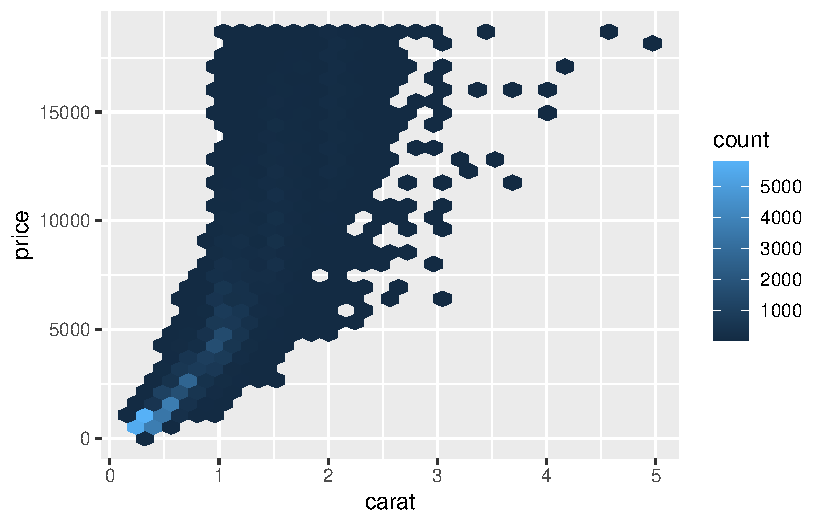
\includegraphics{src/r-for-data-science/06-workflow-scripts-and-projects_files/figure-pdf/unnamed-chunk-3-1.pdf}

\begin{Shaded}
\begin{Highlighting}[]
\CommentTok{\# ggsave("figures/diamonds.png")}

\CommentTok{\# write\_csv(diamonds, "data/diamonds.csv")}
\end{Highlighting}
\end{Shaded}

\chapter{Data Import}\label{data-import}

\section*{Clear Workspace, DON'T
EDIT}\label{clear-workspace-dont-edit-8}
\addcontentsline{toc}{section}{Clear Workspace, DON'T EDIT}

\markright{Clear Workspace, DON'T EDIT}

Always start by clearing the workspace. This ensure objects created in
other files are not used used here.

\begin{Shaded}
\begin{Highlighting}[]
\FunctionTok{rm}\NormalTok{(}\AttributeTok{list =} \FunctionTok{ls}\NormalTok{())}
\end{Highlighting}
\end{Shaded}

\section*{List Used Packages, EDIT}\label{list-used-packages-edit-8}
\addcontentsline{toc}{section}{List Used Packages, EDIT}

\markright{List Used Packages, EDIT}

List all the packages that will be used in chunk below.

\begin{Shaded}
\begin{Highlighting}[]
\NormalTok{packages }\OtherTok{\textless{}{-}} \FunctionTok{c}\NormalTok{()}
\end{Highlighting}
\end{Shaded}

\section*{Load Packages, DON'T EDIT}\label{sec-packages}
\addcontentsline{toc}{section}{Load Packages, DON'T EDIT}

\markright{Load Packages, DON'T EDIT}

\subsection*{Install Missing}\label{install-missing-8}
\addcontentsline{toc}{subsection}{Install Missing}

Any missing package will be installed automatically. This ensure
smoother execution when run on another machine.

\begin{tcolorbox}[enhanced jigsaw, coltitle=black, opacityback=0, colback=white, title=\textcolor{quarto-callout-important-color}{\faExclamation}\hspace{0.5em}{Installing Packages on Other People Machine}, titlerule=0mm, bottomtitle=1mm, arc=.35mm, breakable, colbacktitle=quarto-callout-important-color!10!white, toptitle=1mm, left=2mm, bottomrule=.15mm, opacitybacktitle=0.6, toprule=.15mm, leftrule=.75mm, colframe=quarto-callout-important-color-frame, rightrule=.15mm]

Be aware that people may not like installing packages into their machine
automatically. This might break some of their previous code.

\end{tcolorbox}

\begin{Shaded}
\begin{Highlighting}[]
\CommentTok{\# Do NOT modify}
\FunctionTok{install.packages}\NormalTok{(}\FunctionTok{setdiff}\NormalTok{(packages, }\FunctionTok{rownames}\NormalTok{(}\FunctionTok{installed.packages}\NormalTok{())))}
\end{Highlighting}
\end{Shaded}

\subsection*{Load}\label{load-8}
\addcontentsline{toc}{subsection}{Load}

Load all packages

\begin{Shaded}
\begin{Highlighting}[]
\CommentTok{\# Do NOT modify}
\FunctionTok{lapply}\NormalTok{(packages, require, }\AttributeTok{character.only =} \ConstantTok{TRUE}\NormalTok{)}
\end{Highlighting}
\end{Shaded}

\begin{verbatim}
list()
\end{verbatim}

\section{Introduction}\label{introduction-6}

\part{Practice}

This section contains practices for the programming/scripting languages
that I am learning.

\chapter{Topic Modeling in R}\label{topic-modeling-in-r}

\section*{Clear Workspace, DON'T
EDIT}\label{clear-workspace-dont-edit-9}
\addcontentsline{toc}{section}{Clear Workspace, DON'T EDIT}

\markright{Clear Workspace, DON'T EDIT}

Always start by clearing the workspace. This ensure objects created in
other files are not used used here.

\begin{Shaded}
\begin{Highlighting}[]
\FunctionTok{rm}\NormalTok{(}\AttributeTok{list =} \FunctionTok{ls}\NormalTok{())}
\end{Highlighting}
\end{Shaded}

\section*{List Used Packages, EDIT}\label{list-used-packages-edit-9}
\addcontentsline{toc}{section}{List Used Packages, EDIT}

\markright{List Used Packages, EDIT}

List all the packages that will be used in chunk below.

\begin{Shaded}
\begin{Highlighting}[]
\NormalTok{packages }\OtherTok{\textless{}{-}} \FunctionTok{c}\NormalTok{(}\StringTok{"gutenbergr"}\NormalTok{, }\CommentTok{\# download books from Project Gutenberg using book ID}
              \StringTok{"tidyverse"}\NormalTok{,}
              \StringTok{"tidytext"}\NormalTok{,}
              \StringTok{"ggplot2"}\NormalTok{,}
              \StringTok{"stm"}\NormalTok{, }\CommentTok{\# for do topic modeling}
              \StringTok{"quanteda"}\NormalTok{) }\CommentTok{\# great text mining, will be used to structure the input to stm}
\end{Highlighting}
\end{Shaded}

\section*{Load Packages, DON'T EDIT}\label{sec-packages}
\addcontentsline{toc}{section}{Load Packages, DON'T EDIT}

\markright{Load Packages, DON'T EDIT}

\subsection*{Install Missing}\label{install-missing-9}
\addcontentsline{toc}{subsection}{Install Missing}

Any missing package will be installed automatically. This ensure
smoother execution when run by others.

\begin{tcolorbox}[enhanced jigsaw, coltitle=black, opacityback=0, colback=white, title=\textcolor{quarto-callout-important-color}{\faExclamation}\hspace{0.5em}{Installing Packages on Other People Machine}, titlerule=0mm, bottomtitle=1mm, arc=.35mm, breakable, colbacktitle=quarto-callout-important-color!10!white, toptitle=1mm, left=2mm, bottomrule=.15mm, opacitybacktitle=0.6, toprule=.15mm, leftrule=.75mm, colframe=quarto-callout-important-color-frame, rightrule=.15mm]

Be aware the people may not like installing packages into their machine
automatically. This might break some of their previous code.

\end{tcolorbox}

\begin{Shaded}
\begin{Highlighting}[]
\CommentTok{\# Do NOT modify}
\FunctionTok{install.packages}\NormalTok{(}\FunctionTok{setdiff}\NormalTok{(packages, }\FunctionTok{rownames}\NormalTok{(}\FunctionTok{installed.packages}\NormalTok{())))}
\end{Highlighting}
\end{Shaded}

\subsection*{Load}\label{load-9}
\addcontentsline{toc}{subsection}{Load}

Load all packages

\begin{Shaded}
\begin{Highlighting}[]
\CommentTok{\# Do NOT modify}
\FunctionTok{lapply}\NormalTok{(packages, require, }\AttributeTok{character.only =} \ConstantTok{TRUE}\NormalTok{)}
\end{Highlighting}
\end{Shaded}

\begin{verbatim}
[[1]]
[1] TRUE

[[2]]
[1] TRUE

[[3]]
[1] TRUE

[[4]]
[1] TRUE

[[5]]
[1] TRUE

[[6]]
[1] TRUE
\end{verbatim}

\section{Introduction}\label{introduction-7}

An attempt to understand Sherlock Holmes short stories found in
Adventures of Sherlock Holmes book by Arthur Conan Doyle. After
inspecting the table of content, the book seems to have 12 stories, one
story per chapter. The analysis is inspired by
\href{https://juliasilge.com/}{Julia Silge}'s YouTube video
\href{https://www.youtube.com/embed/evTuL-RcRpc}{Topic modeling with R
and tidy data principles}

\section{Download Book}\label{download-book}

\begin{Shaded}
\begin{Highlighting}[]
\CommentTok{\# Download the book, each line of the book is read into a seperate row}
\NormalTok{sherlock\_raw }\OtherTok{\textless{}{-}} \FunctionTok{gutenberg\_download}\NormalTok{(}\DecValTok{48320}\NormalTok{)}
\end{Highlighting}
\end{Shaded}

\begin{verbatim}
Determining mirror for Project Gutenberg from https://www.gutenberg.org/robot/harvest
\end{verbatim}

\begin{verbatim}
Using mirror http://aleph.gutenberg.org
\end{verbatim}

\begin{Shaded}
\begin{Highlighting}[]
\FunctionTok{dim}\NormalTok{(sherlock\_raw)}
\end{Highlighting}
\end{Shaded}

\begin{verbatim}
[1] 12350     2
\end{verbatim}

\begin{Shaded}
\begin{Highlighting}[]
\FunctionTok{head}\NormalTok{(sherlock\_raw)}
\end{Highlighting}
\end{Shaded}

\begin{verbatim}
# A tibble: 6 x 2
  gutenberg_id text                           
         <int> <chr>                          
1        48320 "ADVENTURES OF SHERLOCK HOLMES"
2        48320 ""                             
3        48320 ""                             
4        48320 ""                             
5        48320 ""                             
6        48320 "[Illustration:"               
\end{verbatim}

\begin{Shaded}
\begin{Highlighting}[]
\FunctionTok{tail}\NormalTok{(sherlock\_raw)}
\end{Highlighting}
\end{Shaded}

\begin{verbatim}
# A tibble: 6 x 2
  gutenberg_id text                                                  
         <int> <chr>                                                 
1        48320 "  boisterious fashion, and on the whole _changed to_"
2        48320 "  boisterous fashion, and on the whole"              
3        48320 ""                                                    
4        48320 "  Page 297"                                          
5        48320 "  wrapt in the peaceful beauty _changed to_"         
6        48320 "  rapt in the peaceful beauty"                       
\end{verbatim}

\section{Wrangle: Label Stories}\label{wrangle-label-stories}

\begin{Shaded}
\begin{Highlighting}[]
\NormalTok{sherlock }\OtherTok{\textless{}{-}}\NormalTok{ sherlock\_raw }\SpecialCharTok{\%\textgreater{}\%} 
  
  \CommentTok{\# determine start of each story/chapter}
  \FunctionTok{mutate}\NormalTok{(}\AttributeTok{story =} \FunctionTok{ifelse}\NormalTok{(}\FunctionTok{str\_detect}\NormalTok{(text, }\StringTok{"\^{}(A SCANDAL IN BOHEMIA|THE RED{-}HEADED LEAGUE|A CASE OF IDENTITY|THE BOSCOMBE VALLEY MYSTERY|THE FIVE ORANGE PIPS|THE MAN WITH THE TWISTED LIP|THE ADVENTURE OF THE BLUE CARBUNCLE|THE ADVENTURE OF THE SPECKLED BAND|THE ADVENTURE OF THE ENGINEER’S THUMB|THE ADVENTURE OF THE NOBLE BACHELOR|THE ADVENTURE OF THE BERYL CORONET|THE ADVENTURE OF THE COPPER BEECHES)$"}\NormalTok{), text, }\ConstantTok{NA}\NormalTok{)) }\SpecialCharTok{\%\textgreater{}\%}
  
  \CommentTok{\# determine lines belonging to each story/chapter by}
  \CommentTok{\# filling down the N/A rows of story column}
  \FunctionTok{fill}\NormalTok{(story) }\SpecialCharTok{\%\textgreater{}\%}
  
  \CommentTok{\# remove the part that does not belong to any story/chapter,}
  \CommentTok{\# i.e, the introduction}
  \FunctionTok{filter}\NormalTok{(}\SpecialCharTok{!}\FunctionTok{is.na}\NormalTok{(story)) }\SpecialCharTok{\%\textgreater{}\%}
  
  \CommentTok{\# convert story column to factor}
  \FunctionTok{mutate}\NormalTok{(}\AttributeTok{story =} \FunctionTok{factor}\NormalTok{(story))}
\end{Highlighting}
\end{Shaded}

\section{Wrangle: Put in Tidy Format}\label{wrangle-put-in-tidy-format}

The row of \texttt{text} column contains multiple words/tokens. We want
to put each word/token of each \texttt{text} row into a separate row.
This makes the dataframe follows the tidy format and hence makes it easy
to process.

\begin{Shaded}
\begin{Highlighting}[]
\NormalTok{tidy\_sherlock }\OtherTok{\textless{}{-}}\NormalTok{ sherlock }\SpecialCharTok{\%\textgreater{}\%}
  
  \CommentTok{\# number the rows}
  \FunctionTok{mutate}\NormalTok{(}\AttributeTok{line =} \FunctionTok{row\_number}\NormalTok{()) }\SpecialCharTok{\%\textgreater{}\%} 
  
  \CommentTok{\# break the text column into multiple row where each row contain one token}
  \FunctionTok{unnest\_tokens}\NormalTok{(word, text) }\SpecialCharTok{\%\textgreater{}\%} 
  
  \CommentTok{\# remove the stopwords{-}{-}the rows where the word column is a stopword}
  \FunctionTok{anti\_join}\NormalTok{(stop\_words) }\SpecialCharTok{\%\textgreater{}\%} 
  
  \CommentTok{\# remove holmes rows which might affect our topic models}
  \FunctionTok{filter}\NormalTok{(word }\SpecialCharTok{!=} \StringTok{"holmes"}\NormalTok{)}
\end{Highlighting}
\end{Shaded}

\begin{verbatim}
Joining with `by = join_by(word)`
\end{verbatim}

\section{Explore tf-idf}\label{explore-tf-idf}

\begin{itemize}
\tightlist
\item
  To see which words are important in each story/chapter, i.e.,the words
  that appears many times in that story but few or none in the other
  stories.
\item
  tf-idf (term frequency-inverse document frequency) is a great
  exploratory tool before starting with topic modeling
\end{itemize}

\begin{Shaded}
\begin{Highlighting}[]
\NormalTok{tidy\_sherlock }\SpecialCharTok{\%\textgreater{}\%} 
  
  \CommentTok{\# count number of occurrence of words in stories}
  \FunctionTok{count}\NormalTok{(story, word, }\AttributeTok{sort =} \ConstantTok{TRUE}\NormalTok{) }\SpecialCharTok{\%\textgreater{}\%} 
  
  \CommentTok{\# compute and add tf, idf, and tf\_idf values for words}
  \FunctionTok{bind\_tf\_idf}\NormalTok{(word, story, n) }\SpecialCharTok{\%\textgreater{}\%} 
  
  \CommentTok{\# group by story}
  \FunctionTok{group\_by}\NormalTok{(story) }\SpecialCharTok{\%\textgreater{}\%} 
  
  \CommentTok{\# take top 10 words of each story with highest tf\_idf (last column)}
  \FunctionTok{top\_n}\NormalTok{(}\DecValTok{10}\NormalTok{) }\SpecialCharTok{\%\textgreater{}\%} 
  
  \CommentTok{\# unpack}
  \FunctionTok{ungroup}\NormalTok{() }\SpecialCharTok{\%\textgreater{}\%} 
  
  \CommentTok{\# turn words into factors and order them based on their tf\_idf values}
  \CommentTok{\# }\AlertTok{NOTE}\CommentTok{: This will not affect order the dataframe rows which is can be}
  \CommentTok{\#   done via the arrange function}
  \CommentTok{\# }\AlertTok{NOTE}\CommentTok{: Recording the word column this way is for ggplot to visualize them}
  \CommentTok{\#   as desired from top tf\_idf to lowest}
  \FunctionTok{mutate}\NormalTok{(}\AttributeTok{word =} \FunctionTok{reorder}\NormalTok{(word, tf\_idf)) }\SpecialCharTok{\%\textgreater{}\%} 
  
  \CommentTok{\# plot}
  \FunctionTok{ggplot}\NormalTok{(}\FunctionTok{aes}\NormalTok{(word, tf\_idf, }\AttributeTok{fill =}\NormalTok{ story)) }\SpecialCharTok{+}
  \FunctionTok{geom\_col}\NormalTok{(}\AttributeTok{show.legend =} \ConstantTok{FALSE}\NormalTok{) }\SpecialCharTok{+}
  \FunctionTok{facet\_wrap}\NormalTok{(}\SpecialCharTok{\textasciitilde{}}\NormalTok{story, }\AttributeTok{scales =} \StringTok{"free"}\NormalTok{, }\AttributeTok{ncol =} \DecValTok{3}\NormalTok{) }\SpecialCharTok{+}
  \FunctionTok{theme}\NormalTok{(}\AttributeTok{strip.text.x =} \FunctionTok{element\_text}\NormalTok{(}\AttributeTok{size =} \DecValTok{5}\NormalTok{)) }\SpecialCharTok{+}
  \FunctionTok{coord\_flip}\NormalTok{()}
\end{Highlighting}
\end{Shaded}

\begin{verbatim}
Selecting by tf_idf
\end{verbatim}

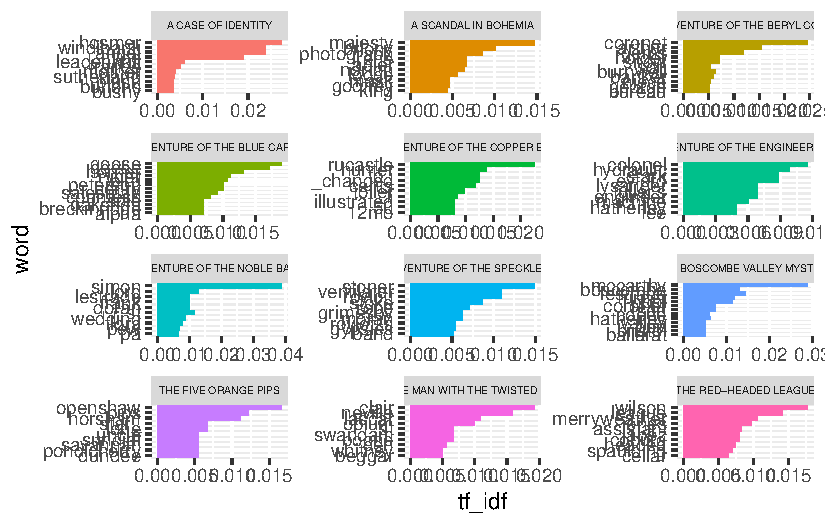
\includegraphics{src/practice/topic-modeling-r_files/figure-pdf/unnamed-chunk-6-1.pdf}

\section{Implement Topic Modeling}\label{implement-topic-modeling}

Training the model for the topics

\begin{Shaded}
\begin{Highlighting}[]
\CommentTok{\# Convert from tidy form to quanteda form (document x term matrix)}
\NormalTok{sherlock\_stm }\OtherTok{\textless{}{-}}\NormalTok{ tidy\_sherlock }\SpecialCharTok{\%\textgreater{}\%} 
  \FunctionTok{count}\NormalTok{(story, word, }\AttributeTok{sort =} \ConstantTok{TRUE}\NormalTok{) }\SpecialCharTok{\%\textgreater{}\%} 
  \FunctionTok{cast\_dfm}\NormalTok{(story, word, n)}

\CommentTok{\# Train the model}
\NormalTok{topic\_model }\OtherTok{\textless{}{-}} \FunctionTok{stm}\NormalTok{(sherlock\_stm, }\AttributeTok{K=}\DecValTok{6}\NormalTok{, }\AttributeTok{init.type =} \StringTok{"Spectral"}\NormalTok{)}
\end{Highlighting}
\end{Shaded}

\begin{verbatim}
Beginning Spectral Initialization 
     Calculating the gram matrix...
     Finding anchor words...
    ......
     Recovering initialization...
    .............................................................................
Initialization complete.
............
Completed E-Step (0 seconds). 
Completed M-Step. 
Completing Iteration 1 (approx. per word bound = -7.785) 
............
Completed E-Step (0 seconds). 
Completed M-Step. 
Completing Iteration 2 (approx. per word bound = -7.593, relative change = 2.458e-02) 
............
Completed E-Step (0 seconds). 
Completed M-Step. 
Completing Iteration 3 (approx. per word bound = -7.481, relative change = 1.473e-02) 
............
Completed E-Step (0 seconds). 
Completed M-Step. 
Completing Iteration 4 (approx. per word bound = -7.455, relative change = 3.469e-03) 
............
Completed E-Step (0 seconds). 
Completed M-Step. 
Completing Iteration 5 (approx. per word bound = -7.450, relative change = 7.612e-04) 
Topic 1: st, simon, lord, day, lady 
 Topic 2: door, miss, house, rucastle, matter 
 Topic 3: hat, goose, stone, bird, geese 
 Topic 4: father, time, mccarthy, son, hand 
 Topic 5: house, time, night, door, heard 
 Topic 6: red, time, wilson, business, headed 
............
Completed E-Step (0 seconds). 
Completed M-Step. 
Completing Iteration 6 (approx. per word bound = -7.449, relative change = 1.233e-04) 
............
Completed E-Step (0 seconds). 
Completed M-Step. 
Completing Iteration 7 (approx. per word bound = -7.449, relative change = 1.168e-05) 
............
Completed E-Step (0 seconds). 
Completed M-Step. 
Model Converged 
\end{verbatim}

\begin{Shaded}
\begin{Highlighting}[]
\FunctionTok{summary}\NormalTok{(topic\_model)}
\end{Highlighting}
\end{Shaded}

\begin{verbatim}
A topic model with 6 topics, 12 documents and a 7709 word dictionary.
\end{verbatim}

\begin{verbatim}
Topic 1 Top Words:
     Highest Prob: st, simon, lord, day, lady, found, matter 
     FREX: simon, clair, neville, lascar, opium, doran, flora 
     Lift: aloysius, ceremony, doran, millar, 2_s, aberdeen, absurdly 
     Score: simon, st, clair, neville, _danseuse_, lestrade, doran 
Topic 2 Top Words:
     Highest Prob: door, miss, house, rucastle, matter, street, lady 
     FREX: rucastle, hosmer, hunter, angel, windibank, _changed, 1 
     Lift: advertised, angel, annoyance, brothers, employed, factor, fowler 
     Score: rucastle, hosmer, angel, windibank, hunter, type, 1 
Topic 3 Top Words:
     Highest Prob: hat, goose, stone, bird, geese, baker, sir 
     FREX: geese, horner, ryder, henry, peterson, salesman, countess 
     Lift: battered, bet, bred, brixton, cosmopolitan, covent, cream 
     Score: goose, geese, horner, _alias_, ryder, henry, peterson 
Topic 4 Top Words:
     Highest Prob: father, time, mccarthy, son, hand, lestrade, left 
     FREX: mccarthy, pool, boscombe, openshaw, pips, horsham, turner 
     Lift: bone, dundee, horsham, pondicherry, presumption, savannah, sundial 
     Score: mccarthy, pool, lestrade, boscombe, openshaw, _détour_, turner 
Topic 5 Top Words:
     Highest Prob: house, time, night, door, heard, hand, round 
     FREX: coronet, stoner, arthur, roylott, ventilator, gems, stoke 
     Lift: _absolute_, _all_, _en, 1100, 16a, 3d, 4000 
     Score: coronet, arthur, stoner, gems, 4000, roylott, ventilator 
Topic 6 Top Words:
     Highest Prob: red, time, wilson, business, headed, day, league 
     FREX: wilson, league, merryweather, jones, coburg, jabez, headed 
     Lift: daring, saturday, vincent, _employé_, _october, _partie, 17 
     Score: wilson, league, merryweather, _employé_, jones, headed, coburg 
\end{verbatim}

\section{Contribution of Words in
Topics}\label{contribution-of-words-in-topics}

Looking at which words contribute the most in each topic.

\begin{Shaded}
\begin{Highlighting}[]
\CommentTok{\# Extracting betas and putting them in a tidy format}
\NormalTok{tm\_beta }\OtherTok{\textless{}{-}} \FunctionTok{tidy}\NormalTok{(topic\_model)}

\CommentTok{\# Visualizing the top words contributing to each topic}
\NormalTok{tm\_beta }\SpecialCharTok{\%\textgreater{}\%} 
  \FunctionTok{group\_by}\NormalTok{(topic) }\SpecialCharTok{\%\textgreater{}\%} 
  \CommentTok{\# top 10 word in each topic with higest beta (last column)}
  \FunctionTok{top\_n}\NormalTok{(}\DecValTok{10}\NormalTok{) }\SpecialCharTok{\%\textgreater{}\%} 
  \FunctionTok{ungroup}\NormalTok{() }\SpecialCharTok{\%\textgreater{}\%} 
  \CommentTok{\# turn words into factors and order them based on their tf\_idf values}
  \CommentTok{\# }\AlertTok{NOTE}\CommentTok{: This will not affect order the dataframe rows which is can be}
  \CommentTok{\#   done via the arrange function}
  \CommentTok{\# }\AlertTok{NOTE}\CommentTok{: Recording the word column this way is for ggplot to visualize them}
  \CommentTok{\#   as desired from top tf\_idf to lowest}
  \FunctionTok{mutate}\NormalTok{(}\AttributeTok{term =} \FunctionTok{reorder}\NormalTok{(term, beta)) }\SpecialCharTok{\%\textgreater{}\%} 
  \FunctionTok{ggplot}\NormalTok{(}\FunctionTok{aes}\NormalTok{(term, beta, }\AttributeTok{fill =}\NormalTok{ topic)) }\SpecialCharTok{+}
  \FunctionTok{geom\_col}\NormalTok{(}\AttributeTok{show.legend =} \ConstantTok{FALSE}\NormalTok{) }\SpecialCharTok{+}
  \FunctionTok{facet\_wrap}\NormalTok{(}\SpecialCharTok{\textasciitilde{}}\NormalTok{topic, }\AttributeTok{scales =} \StringTok{"free"}\NormalTok{, }\AttributeTok{ncol =} \DecValTok{3}\NormalTok{) }\SpecialCharTok{+}
  \FunctionTok{coord\_flip}\NormalTok{()}
\end{Highlighting}
\end{Shaded}

\begin{verbatim}
Selecting by beta
\end{verbatim}

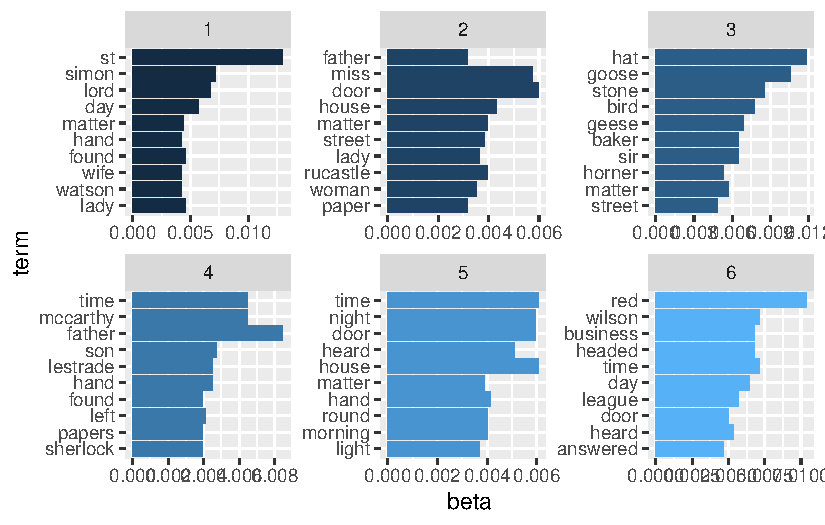
\includegraphics{src/practice/topic-modeling-r_files/figure-pdf/unnamed-chunk-9-1.pdf}

\section{Distribution of Topics in
Stories}\label{distribution-of-topics-in-stories}

Looking at how the stories are associated with each topic and how strong
each association is.

\begin{Shaded}
\begin{Highlighting}[]
\CommentTok{\# Extracting gammas and putting them in a tidy format}
\NormalTok{tm\_gamma }\OtherTok{\textless{}{-}} \FunctionTok{tidy}\NormalTok{(topic\_model, }\AttributeTok{matrix =} \StringTok{"gamma"}\NormalTok{,}
                 \CommentTok{\# use the names of the stories instead of the default numbers}
                 \AttributeTok{document\_names =} \FunctionTok{rownames}\NormalTok{(sherlock\_stm))}


\CommentTok{\# Visualizing the number of stories belonging to each topics and the confidence}
\CommentTok{\#   of the belonging}
\NormalTok{tm\_gamma }\SpecialCharTok{\%\textgreater{}\%} 
  \FunctionTok{ggplot}\NormalTok{(}\FunctionTok{aes}\NormalTok{(gamma, }\AttributeTok{fill =} \FunctionTok{as.factor}\NormalTok{(topic))) }\SpecialCharTok{+}
  \FunctionTok{geom\_histogram}\NormalTok{(}\AttributeTok{show.legend =} \ConstantTok{FALSE}\NormalTok{) }\SpecialCharTok{+}
  \FunctionTok{facet\_wrap}\NormalTok{(}\SpecialCharTok{\textasciitilde{}}\NormalTok{topic, }\AttributeTok{ncol =} \DecValTok{3}\NormalTok{)}
\end{Highlighting}
\end{Shaded}

\begin{verbatim}
`stat_bin()` using `bins = 30`. Pick better value with `binwidth`.
\end{verbatim}

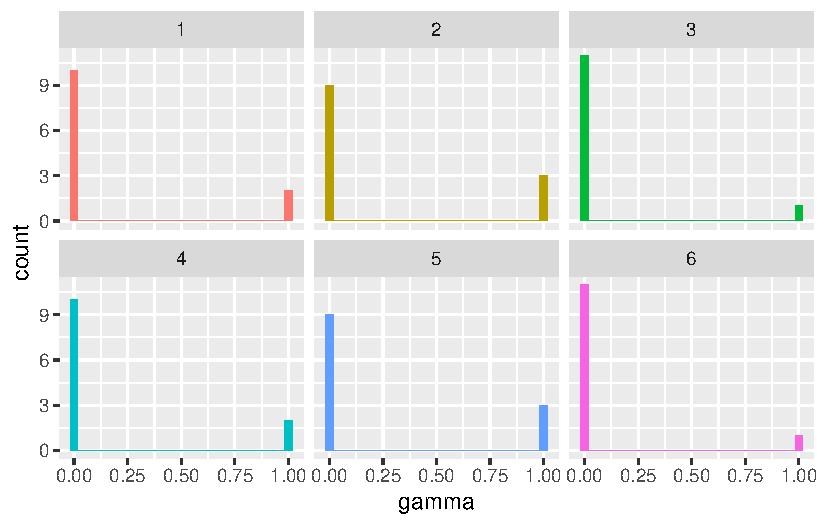
\includegraphics{src/practice/topic-modeling-r_files/figure-pdf/unnamed-chunk-10-1.pdf}

\begin{Shaded}
\begin{Highlighting}[]
\CommentTok{\# Visualizing how much each topic appear in each story}
\NormalTok{tm\_gamma }\SpecialCharTok{\%\textgreater{}\%} 
  \FunctionTok{ggplot}\NormalTok{(}\FunctionTok{aes}\NormalTok{(topic, gamma, }\AttributeTok{fill =}\NormalTok{ document)) }\SpecialCharTok{+}
  \FunctionTok{geom\_col}\NormalTok{(}\AttributeTok{show.legend =} \ConstantTok{FALSE}\NormalTok{) }\SpecialCharTok{+}
  \FunctionTok{facet\_wrap}\NormalTok{(}\SpecialCharTok{\textasciitilde{}}\NormalTok{document, }\AttributeTok{scales =} \StringTok{"free"}\NormalTok{, }\AttributeTok{ncol =} \DecValTok{3}\NormalTok{) }\SpecialCharTok{+}
  \FunctionTok{theme}\NormalTok{(}\AttributeTok{strip.text.x =} \FunctionTok{element\_text}\NormalTok{(}\AttributeTok{size =} \DecValTok{5}\NormalTok{))}
\end{Highlighting}
\end{Shaded}

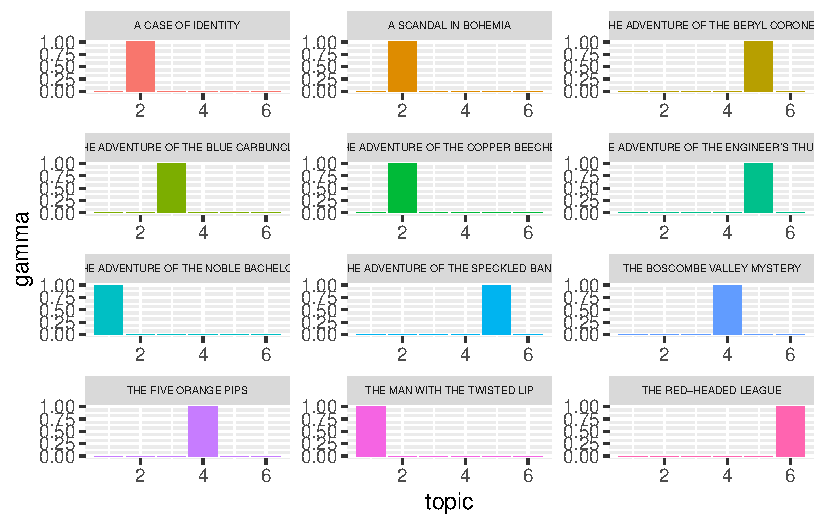
\includegraphics{src/practice/topic-modeling-r_files/figure-pdf/unnamed-chunk-11-1.pdf}

The model did an excellent job strongly associating the stories into one
or more topics. This perfect association is rare in the world of topic
modeling. The reason behind this perfect association here could be due
to the small number of documents that we have.

\section{References}\label{references-2}

\begin{itemize}
\tightlist
\item
  Adventures of Sherlock Holmes book by Arthur Conan Doyle on
  \href{https://www.gutenberg.org/ebooks/48320}{Project Gutenberg}
\item
  \href{https://regex101.com/}{Regular Expressions 101}
\end{itemize}



\end{document}
